% ---- ETD Document Class and Useful Packages ---- %
\documentclass{ucetd}
\usepackage{subfigure,epsfig,amsfonts}
\usepackage{natbib}
\usepackage{amsmath}
\usepackage{amssymb}
\usepackage{amsthm}
\usepackage{subfiles}
\usepackage{standalone}
\usepackage{booktabs}
\usepackage{tabularx}
\usepackage{caption}
\DeclareCaptionFont{mysize}{\fontsize{10}{9.6}\selectfont}
\captionsetup{font=mysize}
%\usepackage[CaptionAfterwards]{fltpage}
%\usepackage[font=scriptsize]{caption}
%\captionsetup[figure]{labelfont=bf}
\captionsetup[figure]{labelfont=bf,labelsep=period}
\graphicspath{ {figures/ch1/}{figures/ch2/}{figures/ch3/}{figures/ch4/} }



%Added 8/30/2015
\makeatletter
\setlength{\@fptop}{0pt}
\makeatother



%Make sure the list of figures has normal font 
% http://tex.stackexchange.com/questions/131930/remove-font-styles-in-list-of-figures
\AtBeginDocument{
  \addtocontents{lof}{%
    \let\sffamily\rmfamily
    \let\scshape\rmfamily
    \let\textbf\textrm
    \let\textit\textrm
  }
}


%% Use these commands to set biographic information for the title page:
\title{Dynamic control of pulsed contractions in the early C. elegans embryo}
\author{Jonathan Brian Michaux}
%\division{Biological Sciences and the Pritzker School of Medicine}
\division{}
\department{Molecular Genetics and Cell Biology}
\degree{Doctor of Philosophy}
\date{March 2017}

%% Use these commands to set a dedication and epigraph text
\dedication{To my parents and my three sisters for all of their support}
\epigraph{Epigraph Text}


\begin{document}
%% Basic setup commands
% If you don't want a title page comment out the next line and uncomment the line after it:
\maketitle
%\omittitle

% These lines can be commented out to disable the copyright/dedication/epigraph pages
\makecopyright
\makededication
%\makeepigraph


%% Make the various tables of contents
\tableofcontents
\listoffigures
\listoftables

%create a list of movies/video
%\listofmovies

%\acknowledgments
% Enter Acknowledgements here

\abstract
% Enter Abstract here
Epithelial morphogenesis consists of the various process that promote the bending, folding, and rearrangement of tissues during organ formation and development.  At the heart of these processes, complex organizations and contractions of the actomyosin cytoskeleton drive the individual cell shape changes that underlie tissue morphogenesis.  The assembly and dynamics of these actomyosin networks are regulated by a host of actin-binding proteins, as well as regulatory molecules such as the RhoA Family of GTPases.  Although much is known about the structure and function of the individual components of contractile networks, much less is known about how cells tune the organization and dynamics these networks in space and in time.  The subject of this thesis is one mode of contractility known as pulsed contractility.  Pulsed contractions have been shown to be a key regulator in various instances of tissue morphogenesis.  We have shown that autocatalytic activation of active RhoA drives pulsed contractions in the early \textit{C.elegans} embryo.  The accumulation of active RhoA precedes the activation, assembly, and recruitment of F-actin, Myosin II, and Anillin within pulsed contractions.  We have also shown that pulses of active RhoA do not depend on the presence of Myosin II or Anillin.  The delayed accumulation of the redundant RhoA GAPs RGA-3 and RGA-4 relative to active RhoA, and the loss of active RhoA pulses in \textit{rga-3/4} mutants, is consistent with RGA-3/4-mediated negative feedback terminating RhoA pulses.  The fact that GFP::RGA-3 strongly co-localizes with F-actin, and the depolymerization of F-actin leads to a near-total loss of GFP::RGA-3 on the cortex and global activation of RhoA, suggests that F-actin mediates this negative feedback.  We believe that the results presented here lay the foundation for a novel conceptual framework in which the spatial and temporal kinetics of RhoA activation is tightly coupled to the dynamics of the underlying actomyosin cytoskeleton.


\mainmatter
% Main body of text follows

% ---- ETD Document Class and Useful Packages ---- %
\documentclass{ucetd}
\usepackage{subfigure,epsfig,amsfonts}
\usepackage{natbib}
\usepackage{amsmath}
\usepackage{amssymb}
\usepackage{amsthm}
\graphicspath{ {figures/ch1/} }
\begin{document}


\chapter{Introduction}
\section{Background}
%Brief intro to quantitative Biology
Biologists have long been fascinated by the myriad beautiful movements that give form and function to developing organisms \cite{Thompson:1917up}.  Starting from a single fertilized embryo, cell growth, cell division, cell migration, and various cell shape changes facilitate the formation of increasingly complex tissues and organs.  Using ideas from classical physics, early researchers during the so-called \textit{Entwicklungsmechanik} (developmental mechanics) period sought to explain how mechanical forces such as spring forces, osmotic pressure, shear stresses, and surface tension can drive various tissue movements during embryonic development.  During the early 1950's, the field of developmental biology took a large step forward when the great mathematician Alan Turing published his seminal paper on morphogenesis \cite{Turing:1952vn}.  Turing demonstrated that a simple system of reacting and diffusing chemical \textit{morphogens} could generate robust spatial patterns \cite{Turing:1952vn}.  It is likely that Turing would have extended his mathematical theory of chemical-based pattern formation to describe the morphogenetic movements of cells and tissues were it not for his untimely death \cite{Turing:1952vn, Howard:2011da}.  Indeed, we now know that the the forces that cells generate, and the resulting embryonic shape changes, are the result of a multitude of interacting components that are both chemically and mechanically regulated \cite{Mammoto:2010bt}.





%Biophysical Tools
Our understanding of embryonic development has greatly improved in the intervening years since the \textit{Entwicklungsmechanik} period.  Decades of research have uncovered many of the key genetic and biochemical pathways underlying the organization of the animal body plan.  Recent advances in light microscopy, the discovery of fluorescent proteins, and the creation of novel biophysical tools now gives researchers unprecedented access to interrogating the inner mechanical and biochemical workings of cells \cite{Heisenberg:2013jk}.  Coupled with high-resolution live imaging, fluorescent probes such as green fluorescent protein (GFP) can be used to assay the expression, activity, and localization patterns of force regulating molecules in cells and tissues.  Particle tracking techniques have been developed to measure the motion of individual proteins, as well as aggregates of molecules.  For example, single-molecule imaging can be used to measure the rates at which various GFP-tagged molecules associate with, and dissociate from, the cell surface \cite{Robin:2014jf}.  Single-molecule imaging can also be used to measure the local cell surface deformation rate during shape changes  (see Chapter 2).  The recent invention of optogenetic probes will also help researchers shed light on the spatial and temporal regulation of signalling pathways that control force generation \cite{Wagner:2016ev}.   Now, one of the major challenges facing cell and developmental biologists will be to use these new tools to understand how the formation of complex tissue architectures is driven by underlying genetic and biochemical mechanisms, as well as the concerted deformation, compression, elongation, and rearrangement of individual cells.




%Specific instances of cell shape changes
Individual cells have the ability to pattern their force-generating machinery in order to change their shape for accomplishing specific tasks \cite{Lecuit:2011ec}.  For example, during cell division an animal cell first rounds up, positions its furrow, and then constricts its membrane in order to split into two daughter cells \cite{Srivastava:2016dm}.  Neuronal cells polarize by extending long axons and several smaller dendrites, thus providing a means for signals to be transmitted throughout the nervous system  \cite{Stiess:2011ji}.  Cell migration, which is important for wound healing, chemotaxis, and immune responses, occurs when a recently polarized cell propels itself forward by forming protrusions to extend its leading edge and by contracting to retract its trailing edge \cite{Mayor:2016iw}.


%Morphogenetic movements that result from specific instances of cell shape changes
Individual cells can also coordinate their shape changes in order to bend, rearrange, elongate, and move epithelial tissues during morphogenesis \cite{Heisenberg:2013jk,Lecuit:2011ec}.  The forces that generate individual cell shape changes are integrated and transmitted throughout a developing tissue by adhesive interactions between neighboring cells, and between cells and external substrates.  For example, apical constriction of epithelial cells is a common morphogenetic movement that has been shown to drive epithelial sheet bending and invagination in diverse developmental contexts such as vertebrate neural tube formation and gastrulation in \textit{Drosophila melanogaster} and \textit{Caenorhabditis elegans} \cite{Sawyer:2010ku,Keller:2011dm}.  Spatiotemporal coordination of epithelial cell migration is one of the key requirements for proper cell intercalation, which is thought to drive tissue narrowing and elongation \cite{WalckShannon:2014go}.  

%Molecular basis for force generation
The various cell shape changes and movements described above all appear to be very different mechanisms that operate in distinct cellular and developmental contexts.  However, much experimental work has demonstrated that all of these cells use cortical actomyosin networks to generate the forces necessary to change their shape \cite{Lecuit:2007cw,Salbreux:2012bo}.  Cortical actomyosin networks sit just below the membrane of embryonic and epithelial cells, and are composed of non-muscle myosin II motors, actin filaments, and a host of bundling, cross-linking, capping, and severing proteins \cite{Levayer:2012bu,Murrell:2015kt}.  Like the sarcomeric structures found in muscle cells, cortical actomyosin networks generate force when non-muscle myosin II uses the energy from ATP hydrolysis to slide actin filaments of opposite polarity past each other.  However, unlike the relatively stable sarcomeres, the individual components of cortical actomyosin networks are constantly turning over and being redistributed whenever the network generates force.  This allows cells to rapidly reorganize their cortical actomyosin networks into structures such as cytokinetic rings, branched lamellar networks, and stress fibers.  Recent evidence suggests that force generation within cortical actomyosin networks might also regulate the distribution of biochemical regulators of contractility \cite{Munro:2004jk}.  Therefore, understanding how local force generation leads to cell shape changes will require a study of the interplay between biochemical signalling and cortical actomyosin contractility. 


%The purpose of this thesis
The subject of this thesis is an increasingly common form of cell shape change known as pulsatile shape change, or pulsed contractility \cite{Munro:2004jk,Martin:2009du,Gorfinkiel:2016bv}.  Pulsatile cell shape changes have been observed during various developmental events such as gastrulation in \textit{Drosophila} and \textit{C. elegans}, compaction of the early mouse embryo, and convergence extension in \textit{Xenopus} \cite{Martin:2009du, RohJohnson:2012cf,Maitre:2015hc}.  The purpose of the remainder of this chapter is to provide a biological context for the novel findings reported in this dissertation.  First, I will provide an overview of the structure and regulation of various components of the actomyosin cortex.  Second, I will provide a brief review of the recent pulsed contraction literature during early \textit{Drosophila} development.  Then, I will describe conceptual and mathematical models that others in the field have proposed to describe the initiation and termination of pulsed contractions.  Finally, I will give a preview of the approach that I (in collaboration with members of the Munro lab) have taken to uncovering important mechanisms regulating pulsed contractility.



\section{Assembly and regulation of actomyosin networks}

\subsection{Structure and regulation of Myosin II}

%Myosin overview
Myosins are a diverse superfamily of actin-based molecular motor proteins that regulate force generation and translocation in cells and tissues \cite{Sellers:2000ub,VicenteManzanares:2009ik}.  A comparative genomic analysis has revealed that there are at least 35 different myosin classes, 13 of which are found in humans \cite{Odronitz:2007hn,Sweeney:2010fg}.  Most myosins consist of an N-terminal head or motor domain, a neck domain, and a C-terminal tail domain \cite{Mooseker:2007ij}.  The head domain binds and hydrolyzes ATP in an actin-dependent manner.  The neck domain contains one or more IQ motifs which bind calmodulin family proteins, such as myosin light chains.  In some cases, different IQ motifs within a single myosin are able to simultaneously bind different light chains (e.g. class II myosins).  The tail domains function by binding cargo for intracellular transport and/or promoting the dimerization of the heavy chain \cite{Sellers:2000ub}.  Myosins within each class often share a similar tail structure \cite{Krendel:2005ko}.  At the molecular scale, myosin motors exhibit a wide range of dynamic behaviors that include sliding, pulling, and walking along actin filaments.  These molecular behaviors translate into the different myosins regulating many different processes such as muscle contraction, cell division, cell migration, adhesion, cell polarity, intracellular trafficking, and organelle positioning \cite{Sellers:2000ub,VicenteManzanares:2009ik}.  



%Power stroke, duty ratio, and 
All myosin motors use a conserved mechanism to convert chemical energy into mechanical energy by coupling ATP hydrolysis to cycles of actin attachment and detachment \cite{DeLaCruz:2004fq}.  In the presence of ADP (i.e., the absence of hydrolyzable ATP), the myosin motor domain binds tightly to an actin filament.  The subsequent exchange of ADP for ATP induces a conformational change that weakens the motor domain's affinity for actin, which causes myosin to detach from actin.  A conformational change then promotes ATP hydrolysis into ADP and inorganic phosphate, and myosin re-attachment to actin.  Finally, the release of inorganic phosphate accompanies the force-generating power stroke.  The cycle starts over when ADP is released and is replaced by the binding of a new molecule of ATP.  

All myosins use this basic power stroke mechanism to generate force.  However, different myosin classes tune various kinetic parameters in the cycle such as the rate of ATP hydrolysis, rate of inorganic phosphate release, ADP affinity, and the lifetimes of the intermediate states.  The duty ratio is another important parameter that is useful for functional comparisons of different myosin motors.  In the case of single motors, it is the fraction of time it remains bound to actin during a single ATP hydrolysis cycle.  In the case asynchronous multi-head ensembles, the duty ratio is the fraction of myosin heads that are attached to an actin filament at any given time.  Measurements from multiple studies have shown that duty ratios vary considerably between myosins \cite{OConnell:2007hb}.  By tuning the duty ratio and other kinetic parameters, various myosins differ in their speed and duration of walking along actin filaments, as well as the amount of force they can generate.

% %Myosin V as an example.
% One interesting example (for conceptual comparisons to class II myosins) is the unconventional class V myosin.  Myosin V is a barbed-end directed motor that is capable of walking great distances along actin filaments.  As a result, myosin V functions during intracellular cargo transport \cite{Hammer:2012dn}.  A detailed kinetic analysis revealed that myosin V has a high affinity for ADP, rapidly hydrolyzes ATP, rapidly releases inorganic phosphate when bound to actin, and as a result has a high duty ratio (~0.7) \cite{DeLaCruz:1999ug}.  These results are in agreement with myosin V being highly processive.  Indeed, a highly processive motor would need to spend a significant fraction of its ATPase cycle bound to actin to prevent diffusion.  In a classic study, Rock \textit{et al.} confirmed that myosin V is highly processive in a series of gliding filament experiments \cite{Rock:2000kl}.  In these assays, myosin motors were attached to a coverslip, fluorescently labeled actin filaments were flowed in, and in the presence of ATP the velocity of myosin is inferred from the velocity of the gliding actin filament \cite{Kron:1986vv}.  Rock \textit{et al.} showed that myosin V's velocity was largely independent of its concentration, suggesting that at low concentrations single myosin V molecules walk processively along an actin filament.  Myosin V's walking behavior has also been visually confirmed \textit{in vitro}.  Using high-speed atomic force microscopy, Kodera \textit{et al.} observed single myosin V molecules walking in a hand-over-hand fashion along an actin filament \cite{Kodera:2010cj}.


%Structure and function class II muscle myosins
Although there are many classes of myosins, the most well known are the ubiquitous class II myosins.  Class II myosins are hexamers that consist of two myosin heavy chains, two essential light chains, and two regulatory light chains (Figure 1.1A).  The heavy chain contains an N-terminal globular head domain with binding sites for ATP and filamentous actin, two adjacent IQ motifs which bind essential and regulatory light chains, and a C-terminal $\alpha$-helical tail that promotes the formation of Myosin II homodimers via coiled-coil interactions. The regulatory light chain regulates Myosin II activity, whereas the essential light chain functions to stabilize the heavy chain.  Myosin II homodimers have a low duty ratio ($\sim$0.04 for skeletal muscle Myosin II and ~0.05 smooth muscle Myosin II), and are thus only weakly processive \cite{Harris:1993tw, OConnell:2007hb}.  This was confirmed by Toyoshima \textit{et al.} in a gliding filament assay, where they discovered that there exists a threshold concentration of the skeletal muscle Myosin II homodimer fragment (HMM) below which actin filaments quickly diffuse away from the surface \cite{Toyoshima:1987kf}.  Instead, Myosin II only becomes highly processive by assembling into bipolar minifilaments containing hundreds of myosin heads (Figure 1.1B).  Skeletal muscle Myosin II minifilaments, along with thin actin filaments, are major components of the historically well-studied sarcomere found in skeletal and cardiac muscle tissue \cite{Huxley:2004he}.  Skeletal muscle Myosin II's low duty ratio is optimal for its function within muscle tissue.  Since each skeletal muscle Myosin II head quickly attaches to, and detaches from, actin filaments, many heads can bind to the same actin filament and produce rapid contractions.  Other class II myosin variants have different duty ratios, and are thus optimized to regulate different biological processes.
%Figure 1.1
\begin{figure}[!htbp]
\centering
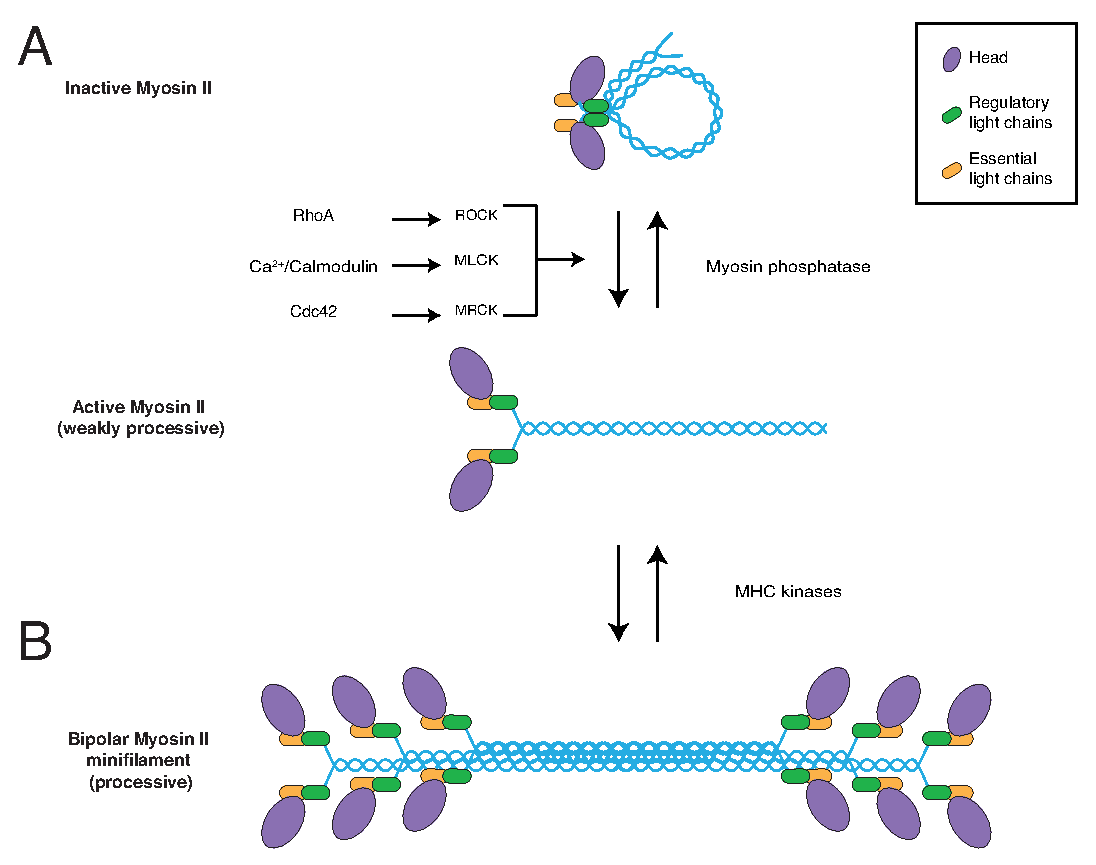
\includegraphics[width=1\textwidth]{Figure1-1}
\captionof{figure}[Structure and assembly of Myosin II minifilaments.]{\textbf{Structure and assembly of Myosin II minifilaments.} (A) When inactive, Myosin II adopts an inhibited folded conformation.  Myosin II is activated by phosphorylation of its regulatory light chain, which induces a conformational change. When active, Myosin II is unipolar and only weakly processive. (B) Phosphorylation of the Myosin II heavy chain controls the assembly of Myosin II into bipolar minifilaments.  In this state, Myosin II motors become highly processive.}
\end{figure}

%Introduction to non-muscle Myosin II (henceforth Myosin II)
 Non-muscle Myosin II is a ubiquitous class II myosin that is found in all eukaryotic cells \cite{Conti:2007hc, VicenteManzanares:2009ik}.  It has been shown to regulate cellular processes such as cell polarity, adhesion, and cell division.  Similar to myosin found in skeletal muscle tissue, non-muscle Myosin II is a hexamer that is highly processive when assembled into bipolar minifilaments.  Unlike skeletal muscle Myosin II, non-muscle Myosin II (henceforth myosin or Myosin II) minifilaments contain far fewer heads.  Based on calculations of the size and shape of minifilaments in their \textit{in vitro} assay, Niederman and Pollard estimated that Myosin II minifilaments derived from human platelet cells contain about 60 heads \cite{Niederman:1975uu}.

%Non-muscle Myosin II regulation
Myosin II activity is primarily regulated by the phosphorylation state of two highly conserved residues (serine 19 and threonine 18 in vertebrates) in the regulatory light chain (RLC) \cite{Moussavi:1993up}.  There are several kinases that have been shown to phosphorylate these residues both \textit{in vitro} and \textit{in vivo}.  These include myosin light chain kinase (MLCK), Rho-kinase (ROCK/Rok), and myotonic dystrophy-related Cdc-42 binding kinase (MLCK), all of which are controlled by members of the family of Rho GTPases \cite{Matsumura:2005cn}.  When the RLC is unphosphorylated, the mysoin II homodimer is autoinhibited by adopting a folded conformation that prevents F-actin binding, ATPase activity, and the formation of minifilaments (Figure 1.1A).  It was first observed in human platelet cells that phosphorylation of serine 19 was shown to significantly increase myosin's actin-dependent ATPase activity \cite{Adelstein:1975vn}.  It was also shown that phosphorylation of serine 19 allowed Myosin II to move actin filaments in \textit{in vitro} gliding assays \cite{Umemoto:1989tw}.  Phosphorylation of both serine 19 and threonine 18 increased enzymatic activity, but not actin filament gliding velocity \textit{in vitro}.  In the context of migrating fibroblasts, mono-phosphorylation of serine 19 promotes adhesion maturation, whereas di-phosphorylation promotes actomyosin bundling in the cell rear \cite{VicenteManzanares:2010gh}.  Phosphorylation of the regulatory light chain is also associated with relieving myosin autoinhibition.  Craig \textit{et al.} showed that phosphorylation of the light chain allows myosin to unfold and adopt an extended conformation (Figure 1.1A) \cite{Craig:1983tq}.  Furthermore, mono- and di-phosphorylation of the regulatory light chain also promoted the assembly of myosin into bipolar minifilaments (Figure 1.1B) \cite{Scholey:1980ui, Ikebe:1988uy}.  Although much less work has been done investigating the role of myosin heavy chain phosphorylation, there exists evidence that phosphorylation of the heavy chain is the major mode of myosin phospho-regulation in \textit{Dictyostelium} \cite{Heissler:2016fs}.


There are three Myosin II isoforms (Myosin IIA-C) in mammalian cells, all of which have different mechanochemistry properties.  While Myosin IIC is not as common, most cells contain Myosin IIA and Myosin IIB \cite{VicenteManzanares:2009ik}.  A detailed kinetic analysis performed by Kovacs \textit{et al.} revealed that the rate of ADP release for Myosin IIA is an order of magnitude greater than its rate of phosphate release \cite{Kovacs:2003ex}.  As a result, Myosin IIA has a low duty ratio that is comparable to that of skeletal muscle Myosin II.  In contrast, another study from the same group showed that the ratio of the rate of ADP release to the rate of phosphate release is much lower in Myosin IIB than that of Myosin IIA \cite{Wang:2003dq}.  Myosin IIB therefore has a higher duty ratio and is capable of exerting greater tension on actin filaments relative to Myosin IIA.  Furthermore, Myosin IIA and Myosin IIB have been shown to have different subcellular localization patterns \cite{Kolega:1998um}.  Combined, these results suggest that Myosin IIA and Myosin IIB might have different functions inside cells.  Indeed, a series of beautiful experiments by Vicente-Manzanares \textit{et al.} demonstrated that although Myosin IIA and Myosin IIB have some overlapping functions, they differentially regulate key aspects of cell migration such as adhesion maturation and rear formation \cite{VicenteManzanares:2007ep, VicenteManzanares:2008kj, VicenteManzanares:2011ha}.  




\subsection{Actin and actin-binding proteins} 
%Actin overview
Actin is a 42-kDa protein that is extremely abundant, highly conserved, and found in nearly all eukaryotic cells.  Like myosin, actin is an ATP binding protein that can assemble into higher order structures. Inside the cell, actin exists in two states: monomeric globular actin (G-actin) and filamentous actin (F-actin).  G-actin undergoes characteristic cycles of assembly into actin filaments, ATP hydrolysis, and disassembly of those filaments.  Actin monomers assemble into polar filaments containing dynamic barbed (plus) and relatively less dynamic pointed (minus) ends.  In filamentous form, actin is one of the major structural components of the cytoskeleton, and is responsible for maintaining cellular tension, generating protrusive forces, and providing tracks for intracellular transport.  The actin cytoskeleton is regulated by a host of nucleation, elongation, branching, capping, bundling, and severing proteins that give rise to rich dynamic properties \cite{Pollard:2016hj}.

%Figure 1.2
\begin{figure}[h!]
\centering
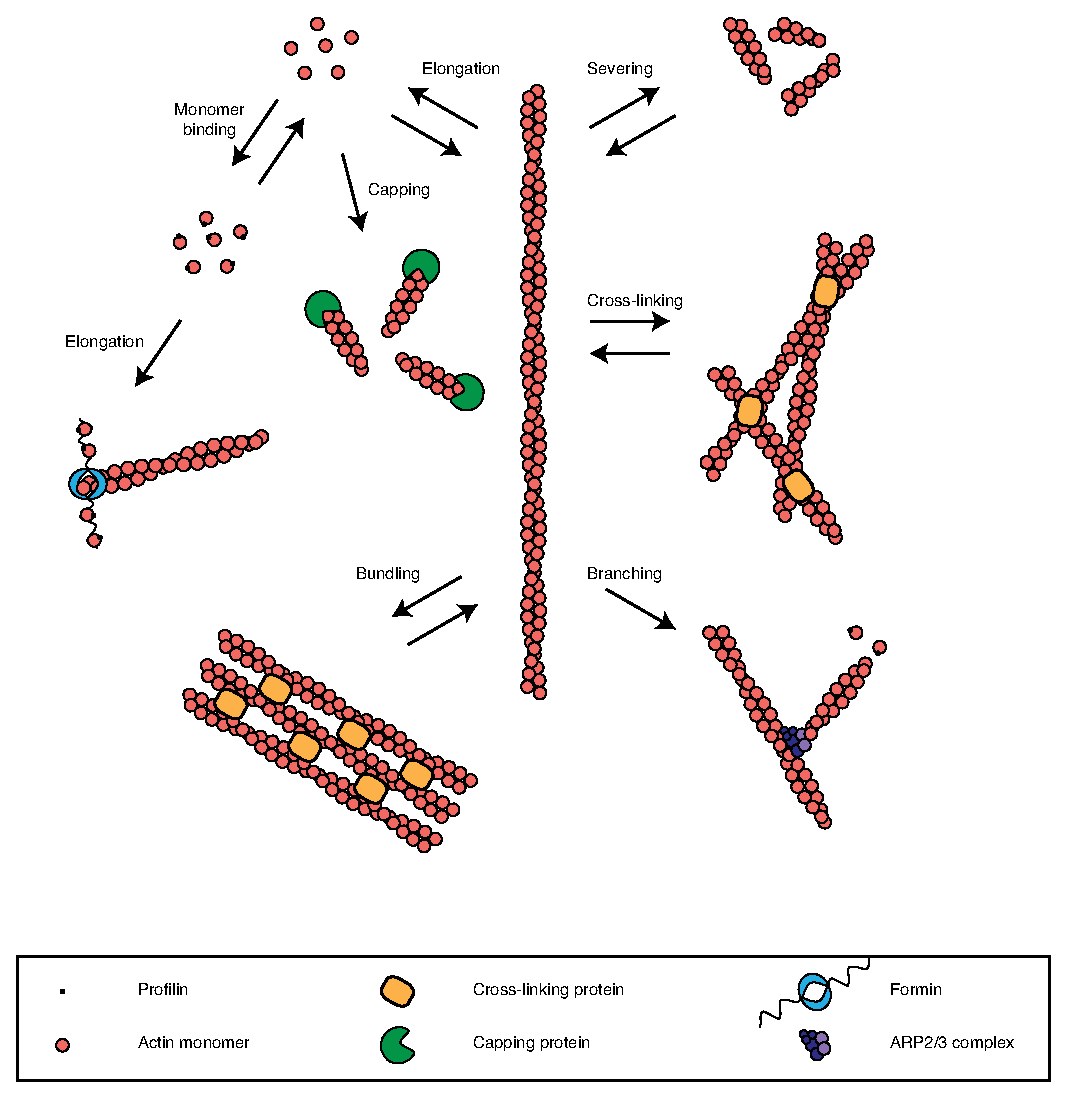
\includegraphics[width=1\textwidth]{Figure1-2}
\captionof{figure}[Overview of actin structures and actin binding proteins.]{\textbf{Overview of actin structures and actin binding proteins.} The structure and dynamics of actin networks is regulated by a host of actin binding proteins that bundle, branch, cross-link, sever, elongate, and cap actin filaments.}
\end{figure}


%Actin assembly and disassembly kinetics
Much of what we know about actin polymerization and depolymerization dynamics has come from \textit{in vitro} studies that monitored actin assembly and disassembly processes in sedimentation, fluorescence spectroscopy, and viscometry assays \cite{Pollard:2016hj}.  Actin polymerization is thought to occur in three sequential stages.  The first stage is the lag period, where actin monomers rapidly associate, often forming unstable oligomers.  Nucleation of actin dimers and trimers is thought to be the rate limiting step of actin polymerization \cite{Cooper:1983uk}.  Thus, the lag period appears to have a strong dependence on actin monomer concentration.  The second stage, which is the elongation stage, occurs when actin oligomers form a stable seed and rapidly elongate.  The third stage occurs when actin monomers and actin filaments have reached a steady state where there is no net polymerization.  The critical concentration of actin is the concentration of unassembled actin monomers in solution after the assembly assay reached steady state.  


%ATP hydrolysis and barbed end growth
Actin polymerization and depolymerization are driven by a complex ATP hydrolysis cycle.  Polymerization of actin filaments primarily occurs by addition of ATP-bound monomeric actin to the fast growing barbed end instead of the slow growing pointed end.  After a monomer has been added, ATP is rapidly hydrolyzed to ADP and inorganic phosphate.  Inorganic phosphate is then slowly released, resulting in ADP-F-actin.  During elongation, more ATP-bound monomers are added to the barbed while older subunits within the actin filament hydrolyze their ATP.  These older ADP-F-actin subunits are readily turned over by depolymerization and severing, and can then be recycled for later incorporation into other actin filaments and networks.


%Thymosin beta 4
The concentration of actin monomers within cells is much greater than the critical concentration required for the spontaneous polymerization of pure actin \textit{in vitro}.  At such high concentrations nearly all of the actin in a cell would be expected to be in filament form.  Instead, cells regulate actin polymerization through a host of actin binding proteins that function to promote or inhibit actin assembly.  One such protein is thymosin-$\beta$-4.  Thymosin-$\beta$-4 is currently thought to be the main actin-sequestering protein in cells \cite{Goldstein:2005kk}.  The concentration of thymosin-$\beta$-4 \textit{in vivo} has been shown to vary from 20$\mu$M in \textit{Xenopus} extracts to 600$\mu$M in platelets, which is at least twice the concentration of unpolymerized monomeric actin \cite{Pollard:2000bla}.  Thymosin-$\beta$-4 binds much more tightly to ATP-bound actin than ADP-bound actin.  When in complex, thymosin-$\beta$-4-bound G-actin cannot associate with the barbed or pointed ends of an actin filament.


%Profilin
Profilin, another actin monomer binding protein, was first characterized in spleen extracts as a small protein whose association with actin could explain actin's ability to persist as monomers under physiological conditions \cite{Carlsson:1977tv}.  Later experiments showed that Acanthamoeba profilin increased the critical concentration of Acanthamoeba actin \cite{Tseng:1982uc}.  Purified profilin was also shown to cause actin filaments at steady-state to depolymerize in a dose-dependent manner \cite{Tseng:1982uc}.  Together, these early results suggested that profilin functions to sequester actin monomers.  However, unlike thymosin-$\beta$-4, profilin is actually thought to promote actin filament assembly.  Indeed, profilin is able to promote addition of monomers selectively to the barbed ends of actin filaments without lowering the critical concentration \cite{Pring:1992us, Pollard:2000bla, Kang:1999wx}.  Furthermore, it has been shown that profilin-actin can be added to actin filament barbed ends with similar kinetics as actin monomers \cite{Kang:1999wx}.  This suggests that profilin maintains a large pool of actin monomers that would readily be incorporated into filaments by binding to any free barbed ends.

%Capping
Since actin filament elongation occurs rapidly at barbed ends, how do cells prevent the pool of actin monomers from being quickly depleted?  One way cells regulate their amount of free actin monomers is by regulating the number of free barbed ends through capping proteins.  It is thought that capping proteins are present at high enough concentrations, and with high enough affinity, to cap most barbed ends \textit{in vivo} \cite{Schafer:1996vi}.  Therefore, the coordinated behavior of capping proteins and actin monomer-binding proteins play an essential role in regulating the pool of actin monomers.


%Severing actin filaments
Cells use another protein known as ADF/Cofilin to regulate the concentration of actin monomers \cite{Hotulainen:2005im}.  ADF/Cofilin is an actin severing protein that is expressed in all eukaryotic cells, with mammalian cells containing three forms known as ADF, cofilin-1,and cofilin-2 \cite{Bernstein:2010cn}.  Cofilin-1,the major form of the protein found in non-muscle tissue, plays an important role in cytokinesis, cell migration, and cancer invasion \cite{Chen:2011jh, Roussos:2011kx}.  \textit{In vitro} studies have shown that low concentrations of cofilin promote actin depolymerization by severing actin filaments \cite{Andrianantoandro:2006hk}.  However, like other actin binding proteins, cofilin's function inside cells is highly complex and depends on its local concentration relative to other actin regulators \cite{Bernstein:2010cn}.  For example, cofilin-mediated severing can also promote actin polymerization by creating free barbed ends \cite{Ichetovkin:2002ur}.  This is important for the polymerization of branched actin networks in the lamellipodium during cell migration \cite{BravoCordero:2013ef}.  At very high concentrations, cofilin is thought to nucleate actin filaments directly \cite{Andrianantoandro:2006hk}.

%ARP-2/3 
Cells employ a variety of mechanisms such as actin-monomer binding, capping, and actin filament severing to prevent spontaneous nucleation of actin filaments.  Cells overcome these inhibitory functions through the use of various factors that catalyze the nucleation and elongation of actin filaments.  The ARP2/3 complex is one of the most abundant and well-understood actin nucleators.  It plays a role in processes such as cell migration, where it has been shown to create dendritic lamellar networks that propel the cell forward.  ARP2/3 was first purified based on its affinity for binding to profilin \cite{Machesky:1994wg}.  Unlike many other actin nucleators, ARP2/3 is unique because it nucleates branched actin filaments by binding to the side of pre-existing filaments.  ARP2/3 binds stably to the mother filament and nucleates a daughter 70$\,^{\circ}$ relative to the axis of the filament.  The ARP2/3 complex consists of seven subunits: ARP2, ARP3, and ARPC1-5 (actin-related protein complex) \cite{Goley:2006cr}.  ARP2 and ARP3 are structurally similar to actin, and also have ATP binding and hydrolysis activity.  ATP binding appears to be important for inducing large scale conformational changes that increase ARP2/3's affinity for nucleation promoting factors (NPFs).  The role of ATP hydrolysis by ARP2 remains unclear, as studies have linked ATP hydrolysis to nucleation and un-branching events \cite{Dayel:2004dy,LeClainche:2003bh}.  A cryo-EM structure of activate ARP2/3 complex suggests that the additional subunits might play a role in mediating contacts with the mother filament \cite{Egile:2005bm}.




%Regulation of ARP-2/3 
ARP2/3 by itself is not an efficient nucleator.  Three of the main regulators of ARP2/3 activity include binding to pre-existing actin filaments, phosphorylation of certain ARP2 (and \textit{maybe} ARP3) residues, and interactions with NPFs such as WAVE and WASP/SCAR \cite{Campellone:2010gd}.  The activity of these NPFs is in turn spatially and temporally regulated by various signal-transduction pathways \cite{Goley:2006cr}.  WASP (Wiskott— Aldrich syndrome protein) and WAVE (WASP-family verprolin-homologous protein) are class I NPFs that share a common WCA domain.  The WCA domain consists of a WASP-homology-2 (WH2) domain, a cofilin-homology (C) domain, and an acidic (A) domain.  The WH2 binds G-actin, while the CA (C and A domain together) region promotes ARP2/3 binding.  \textit{In vitro} studies have shown that the WCA domain is sufficient to activate AP2/3 to polymerize branched actin networks \cite{Goley:2006cr}.  It was originally thought that the WCA simply delivered an actin monomer to the ARP2/3 complex, thus promoting the formation of an actin trimer that can nucleate new branched filaments.  However, recent biochemical and structural studies suggest that the WCA domains of WAVE and WASP regulate a more complex mechanism where the CA domain induces a conformational change in ARP2/3 that brings ARP2 and ARP3 closer together while the WH2 domain delivers the actin monomer.

%Formin and unbranched networks
Unlike the ARP2/3 complex, all other known actin polymerization proteins form unbranched actin filaments.  The most common nucleators are ENA/VASP and formins.  Formins, found in nearly all eukaryotic cells, are both actin nucleators and elongators \cite{Chesarone:2010iw}.  Formins have been shown to build diverse cellular structures such as filopodia, stress fibers, yeast actin cables, and the cytokinetic ring \cite{Suarez:2016bw}.  Formin family proteins are characterized by the highly conserved formin homology domains FH1 and FH2.  Formins can be subdivided into different subclasses based on the divergence of the FH2 sequence \cite{Higgs:2005hn}.  However, sequence differences in the FH1 and FH2 domains of individual formins vary their ability to associate with actin filament barbed ends.  It is thought that these biochemical differences determine whether a a formin is better at nucleating or elongating actin filaments.

The domain organization of formins can be split into two groups: an N-terminal regulatory region that plays a role in localizing formins in vivo and auto-inhibiting its activity, and C-terminal active region that promotes actin filament assembly.  More specifically, the regulatory region of mammalian formins such as mDIA1-3 (similar to \textit{Drosophila} Diaphanous) contains a Rho GTPase-binding domain (GBD), a diaphanous inhibitory domain (DID), and a dimerization and/or coiled-coil domain (CC).  The active region of mammalian formins contains an FH1 domain, an FH2 domain, and diaphanous autoregulatory domain (DAD).  Formin functions as a dimer that changes conformation between an active and inactive state.  \texit{In vitro} experiments have shown that when formin is inactive, interactions between the DAD and DID domains inhibit actin polymerization by the FH2 domain.  In some instances this inhibition can be relieved by the binding of Rho GTPases near the DAD region.  The FH1 domain lacks a well-defined secondary structure, but contains a polyproline region that binds profilin.  The FH2 domain, which nucleates and elongates actin filaments, forms head-to-tail dimers that are topologically similar to a torus \cite{Xu:2004vc}.


%Formin nucleation and elongation
\textit{In vitro} experiments have shown that the FH2 domain is sufficient to nucleate actin filaments even though it has a low affinity for actin monomers  \cite{Pring:2003dw,Sagot:2002is}.  Instead, formin is thought to nucleate actin filaments by binding and stabilizing actin dimers \cite{Pring:2003dw}.  Therefore, the rate-limiting step for actin nucleation is the formation of short-lived actin dimers and trimers.  The FH2 domain does have a high affinity for actin filaments.  Once a stable filament is nucleated, actin can be elongated by formins.  An active formin will enclose the barbed end through interactions between the FH2 domain and the two terminal actin subunits.  These interactions between formin and barbed ends rely on proper dimerization of the FH2 domain.  Elongation then proceeds as formin processively caps and adds monomers to the barbed end.  The FH1 domain also plays a key role in filament elongation.  FH1-profilin interactions are thought to enhance actin filament elongation by increasing the local concentration of actin monomers near the barbed end \cite{Kovar:2006fm, Vavylonis:2006im, Paul:2008kv}.


\subsection{Rho GTPases: Master regulators of actomyosin contractility}
%Overview of Rho Regulating actin networks
The overall structure and contractile properties of actomyosin networks are determined by the regulation of myosin motor activity, the structure and density of the actin network, and the local concentrations actin binding proteins that cap, cross-link, bundle, and sever actin filaments.  Therefore, an unresolved challenge in cell biology is to understand how cells coordinate the activities of these overlapping sets of components in order to regulate the assembly of contractile networks in space and time.  Much research has shown that the Rho family of GTPases, a subfamily of the Ras superfamily, are important regulators of the actin cytoskeleton \cite{Hall:2012cg}.  Rho GTPases act as molecular switches to regulate a wide range of important cellular processes such as cytokinesis, vesicle trafficking, cell migration, and cell shape changes \cite{Piekny:2005dw,Symons:2003vy,Ridley:2001wu, EtienneManneville:2002fq}.  Classic work by Nobes and Hall was the first to demonstrate that the canonical Rho GTPase subclasses RhoA, Rac, and Cdc42 differentially regulate the formation of different actin structures within migrating fibroblasts \cite{Nobes:1995wn}.  They showed that RhoA stimulates the formation of stress fibers and focal adhesions, Rac promotes the formation of the lamellipodia, and Cdc42 promotes the formation of filopodia \cite{Nobes:1995wn}.  Since this discovery, Rho GTPases have been implicated in a diverse range of other processes such as adherens junction remodeling in \textit{Drosophila}, hyper-proliferation of cancer cells and metastatic tumor invasion \cite{Sahai:2002el}, and neurite growth during neuronal development \cite{Stankiewicz:2014bz}.



%Overview
Rho GTPases are monomeric proteins that are about 20kD in size \cite{Schaefer:2014ez}.  Like other GTPases, most Rho GTPases transition between an active conformation when bound to GTP and an inactive conformation when bound to GDP \cite{Hodge:2016cz}.  When active, Rho GTPases initiate signaling through interactions with a host of downstream effectors.  Biochemical studies have shown that Rho GTPases have a high affinity for guanine nucleotides, but intrinsically exchange GTP for GDP slowly \cite{Bos:2007cu}.  In addition, Rho GTPases also hydrolyze GTP slowly.  Therefore, the activity cycle of Rho GTPases is controlled to a large extent by three distinct classes of accessory proteins: GEFs, GAPs, and GDIs.  Guanine nucleotide exchange factors (GEFs) activate Rho GTPases by catalyzing the exchange of GDP for GTP.  They accelerate the rate exchange of GDP for GTP by several orders of magnitude \cite{Vetter:2001iw}.  GTPase activating proteins (GAPs) inactivate Rho GTPases by increasing their intrinsic ability to hydrolyze GTP.  Guanine nucleotide dissociation inhibitors (GDIs) prevent Rho GTPase activation and membrane localization by binding and sequestering the inactive GDP-bound conformation in the cytoplasm \cite{GarciaMata:2011hb}.  In addition, there exists certain post-translational modifications that further regulate the spatial and temporal activation of Rho GTPases \cite{Hodge:2016cz}.  For example, lipid modifications such as C-terminal prenylation localize Rho GTPases to specific membrane compartments. 


%Structure and function of RhoA domains
Along with Rac and Cdc42, RhoA is one of the most studied Rho GTPases.  Madaule and Axel inadvertently identified RhoA in the marine snail \textit{Alypsia} \cite{Madaule:1985wf}.  Since then, other isoforms of RhoA have been identified.  Structurally, RhoA consist of a G domain, a Rho insert region, and a C-terminal hypervariable region.  The G domain consists of five conserved motifs G1-G5.  The G1, G4, and G5 motifs are all involved in nucleotide binding, whereas the G2 and G3 motifs contain switch I and switch II regions, respectively.  The switch I and switch II regions interact with GAPs and GEFs, and change conformation depending on whether GDP or GTP is bound.  The insert region is located between the G4 and G5 regions, and functions to bind GEFs and downstream effectors proteins such as mDia and ROCK \cite{Lammers:2008gi, Zong:2001ho}.  Phosphorylation of the C-terminal hypervariable region appears to play a role in RhoA inactivation by promoting GDI binding and membrane dissociation \cite{Clague:2012gb}.  Next to the hypervariable region, the C-terminus contains a CAAX-box that can be posttranslationally modified by attachment of a lipid anchor.  The lipid anchor plays a role in subcellular localization as well as GDI binding. 




%Short Paragraph on GAPs and GEFs (Upstream)
The activity of RhoA is also determined by the balance between its activators (GEFs) and its inhibitors (GAPs).  There are over 70 different Rho GEFs and about 80 different Rho GAPs in mammals \cite{Cherfils:2013ks}.  GEFs can be classified into two different families, either DBL or DOCK, based on their structure.  DBL-family GEFs are the largest and best understand Rho GEFs \cite{Rossman:2005do}.  They are characterized by a DBL-homology (DH) domain that is associated with a pleckstrin homology (PH) domain.  The DH domain interacts with the switch regions of RhoA to catalyze the exchange of GDP for GTP \cite{Rossman:2005do}.  Variable interactions between the poorly conserved switch-back region of the DH domain and the G domain of RhoA mediates DBL GEF selectivity amongst Rho isoforms \cite{Rossman:2005do, Schaefer:2014ez}.  Like GEF activation, GAP inactivation of RhoA is mediated by interactions with the switch regions \cite{Cherfils:2013ks}.  However, much less is known about how Rho GAPs differentiate between the different Rho isoforms.  The large number of GAPs and GEFs, as well as the variations in their binding and catalytic regions, enumerate the myriad biochemical pathways that RhoA controls \cite{Schaefer:2014ez}.  


%Rho Downstream effectors: ROCK and Dia/%Organization of cortical actomyos
The specific activation, localization, and signalling of RhoA provides a basis for the selective activation and recruitment of specific downstream effector proteins in different cellular contexts.  It is through these effector proteins that RhoA can promote the formation of distinct actomyosin structures.  One important and well-studied example is the assembly and constriction of the contractile ring during cytokinesis.  Cytokinesis involves properly positioning the site of furrow ingression, recruiting factors that promote actin and myosin II assembly into an actomyosin ring, and constricting the membrane to form two daughter cells.  RhoA regulates this complex process by promoting actin filament polymerization and myosin II mini-filament assembly through formin and Rho kinase, respectively.  RhoA has also been shown to recruit the scaffold protein anillin, which might function to stabilize myosin II in the contractile ring \cite{Piekny:2008jf}.  Although there are multiple Rho GTPases involved in cytokinesis, RhoA seems to be the most important \cite{Piekny:2005dw}.  Indeed, RhoA localizes to the furrow independent of actin and myosin, and inhibiting RhoA activity prevents furrow ingression in many different animal cells  \cite{Yuce:2005hz, Piekny:2005dw}.  Furthermore, an important recent study by Wagner and Glotzer showed that local photo-activation of RhoA is sufficient to induce furrow formation \cite{Wagner:2016ev}.  


\section{Review of pulsed contractility}
\subsection{Pulsed contractions are ubiquitous}
%Broad overview of what pulsed contractions are (maybe include a figure)
Pulsed contractility is a common mode of contractility that has been observed in a wide range of contexts.  Pulsed contractions are characterized by cycles of actin assembly and myosin activation, local force generation that transiently deforms cellular surfaces, and disassembly.  Although pulsed contractions were first identified in the early \textit{C. Elegans} embryo, much of what we know about the mechanisms underlying pulsed contractions comes from studies of epithelial morphogenesis during early \textit{Drosophila} development.  During gastrulation, pulsed contractions are thought to play a key role in promoting tissue bending and elongation.  In this section, I review what is currently known about how pulsed contractions drive during mesoderm invagination and germ band elongation in \textit{Drosophila}.


\subsection{Pulsed contractions in \textit{Drosophila} Mesoderm invagination}
%Introduction to Mesoderm invagination
Mesoderm invagination is one of the first steps of \texit{Drosophila} gastrulation.  Early work showed that two transcription factors, \textit{snail} and \textit{twist}, are required for proper development of the mesoderm \cite{Simpson:1983wv}.  In a later study, Leptin and Grunewald made the key observation that both \textit{snail} and \textit{twist} are expressed in the ventral cells in the presumptive mesoderm \cite{Leptin:1990ub}.  They also provided a detailed description of the cell shape changes that occur during mesoderm invagination \cite{Leptin:1990ub}.  Mesoderm invagination can be thought of as a two-step process.  During the first step, ventral cells apically constrict and bend the tissue to form a ventral furrow.  During the second step, the presumptive mesoderm cells spread out under the ectoderm to form the second germ layer.  



%Apical constriction 
Apical constriction is a common cell shape change that occurs in many organisms and during many stages of embryogenesis \cite{Sawyer:2010ku}.  By shrinking its apical surface, a columnar, or cuboidal, epithelial cell can adopt a wedge-shaped geometry that can promote different tissue architectures depending on the developmental context \cite{Martin:2014bi}.  If cells maintain adhesive contacts, coordinated apical constriction can promote bending, folding, and invagination of epithelial tissues.  Apical constriction can also promote cell ingression, extrusion of apoptotic cells, and wound healing \cite{Martin:2014bi}.  Apical constriction was first thought to proceed through a purse-string mechanism, where cell surface deformation is driven by circumferential actin and Myosin II continuously contracting and exerting force on adherens junctions \cite{Lecuit:2007cw}.  This mechanism has been supported by classic studies on \textit{Xenopus} neurulation \cite{Martin:2014bi}.  However, there is also growing evidence that dynamic actomyosin networks on the apical cortex can drive apical constriction \cite{Martin:2014bi,Davidson:2012bf}.  

%Martin et al 2010
Martin \textit{et al.} demonstrated that apical constriction of \textit{Drosophila} ventral cells is not driven by a purse-string mechanism \cite{Martin:2009du}.  Instead, pulsatile contractions of the medioapical cortex shrink the apical surface of ventral cells in a two step ratchet-like manner \cite{Martin:2009du}.  During the first step, known as the constriction phase, a decrease in apical surface area is strongly correlated with a large increase in the constriction rate.  The second step is a stabilization phase, where the previously reduced apical surface area remains constant in the absence of any constriction.  By imaging live cells expressing fluorescent markers for the membrane and Myosin II, they assayed myosin dynamics during apical constriction.  During the constriction phase, the authors observed that pulsed accumulation and coalescence of myosin punctae was also strongly correlated with a decrease in apical surface area.  The accumulation of myosin to the apical surface was mostly medial, and its coalescence into pulses required an intact medioapical actin meshwork.  They also observed a strong correlation between the accumulation rate of myosin and the constriction rate.  The myosin foci then disappeared during the stabilization phase.  

Martin \textit{et al.} confirmed that this two step apical constriction process is under the control of the transcription factors \textit{snail} and \textit{twist} \cite{Martin:2009du}.  They observed that Myosin II pulses did not form in the absence of \textit{snail}, and that ventral cells did not decrease their apical surface area.  In the absence of \textit{twist},  Myosin II  did not localize medioapically, but instead accumulated to the junctions.  The ectopic accumulation of Myosin II to the junctions was associated with transient decreases in cell surface area that were not stabilized.  These results suggest that \textit{snail} is required for the constriction phase, while \textit{twist} is required for the stabilization phase.

In order for ventral furrow cells to decrease their apical surface area through a pulsatile mechanism, contractile actomyosin pulses must transmit forces across adherens junctions.  Furthermore, an intact apical actomyosin network is required to maintain the transient cell shape changes the occur during the stabilization phase between pulses.  How, then, are these apical actomyosin networks assembled and regulated during ventral furrow invagination?  How are apical actomyosin dynamics and adherens junction remodeling coupled?

In a subsequent paper from the Martin group, Mason \textit{et al.} addressed these questions by focusing primarily on factors downstream of Twist activity, namely the GTPase RhoA (Rho1 in \textit{Drosophila}) and its effectors Rok and Dia \cite{Mason:2013ee}.  The authors showed that RhoA, Rok, Myosin II, and Dia all co-localize medioapically in ventral furrow cells \cite{Mason:2013ee}.  They also showed that RhoA, Dia, F-actin, and E-cadherin co-localize in the junctional domains.  Rok activity is required for the proper localization and activation of Myosin II to the apical surface of ventral furrow cells.  The authors confirmed this by inhibiting Rok activity with the Rho kinase inhibitor Y-27632.  Under these conditions, there was  Myosin II no longer formed pulses.  As expected, the loss of myosin pulses prevented the decrease in apical surface area of ventral furrow cells.  Rok activity was also shown to be required for condensing the actin cables that span the apical surface.  These results are consistent with Rok activity being necessary for stabilizing Myosin II pulses and shape changes following pulses.  However, Rok activity is not required  to assemble the medioapical actin network.  Instead, the medioapical actin network is mediated by the formin Dia.  In addition to building the apical actomyosin meshwork, Dia-mediated F-actin polymerization also regulates the localization of E-cadherin.  Indeed, the presence of a partial loss-of-function $\textit{dia}^M$, the authors showed that E-cadherin no longer localized to junctions, but instead localized across the apical surface.

%Paragraph about Twist and snail
How, then, do Twist and Snail coordinate Rok activity, F-actin network assembly and architecture, and E-cadherin dynamics even though these factors localize to separate domains?  The authors demonstrated that Twist and Snail play distinct roles in regulating both F-actin and Rok.  For example, \textit{snail} mutants lack a medioapical actin network as well as junctional F-actin cables.  In addition, in \textit{snail} mutants Rok and Myosin II localize to the subapical junctions instead of the apical surface.  In contrast, \textit{twist} mutants fail to form actin cables that span the apical cortex, and instead form a punctate medioapical actin network.  Furthermore, Rok and Myosin II localize to apical junctions in \textit{twist} mutants.  These observations are consistent with previous work showing \textit{twist} mutants undergoing cycles of pulsatile cell shape change that are not stabilized \cite{Martin:2009du}.  Together, these results suggest a mechanism where Twist spatially and temporally coordinates Myosin II activity, F-actin assembly and junctional remodeling by mediating differential localization of Rok/Myosin II and E-cadherin.  The authors propose that Twist does this by polarizing RhoA activity in the plane of the apical surface.





\subsection{Pulsed contractions in \textit{Drosophila} Germ band elongation}
%Introduction to germ band elongation and cell intercalation in Drosophila 
Germ band extension is a morphological process that gives rise to the thorax and abdomen in \textit{Drosophila}.  Germ band extension starts shortly after the beginning of gastrulation.   Similar to other systems such as \textit{Xenopus} convergent extension and chick neurulation, cellular rearrangements during \textit{Drosophila} germ band extension are mostly driven by cell intercalation \cite{Irvine:1994ug}.  In the \textit{Drosophila} germ band, cells intercalate along the dorsoventral axis.  Other cell shape changes and oriented cell divisions are only thought to contribute a small amount to elongating the tissue \cite{daSilva:2007er}.  One of the hallmarks of germ band extension is the extensive remodelling of adherens junctions between neighboring cells \cite{Bertet:2004ch}.  First, the 'vertical' junctions parallel to the dorso-ventral axis are shortened.  Then, germ band cells transition from having ‘vertical’ type 1 junctions that are perpendicular to the anterior-posterior axis, to having ‘horizontal’ type 3 junctions which are perpendicular to the old type 1 junctions and oriented along the anterior-posterior axis \cite{Bertet:2004ch}.  As a result of these junctional shrinkages, the germ band doubles in length along the anterior-posterior axis, and decreases in width along the dorsoventral axis.


%Pulsed contractions: Rauzzi paper
How are the junctions in the ectoderm remodeled during germ band elongation?  One reasonable hypothesis is that junctional accumulation of Myosin II drives junction shrinkage during cell intercalation.  Indeed, Bertet \textit{et al.} showed that the Myosin II heavy chain (Zip in \textit{Drosophila}) localizes to apical junctions only in the intercalating cells \cite{Bertet:2004ch}.  They also showed cell intercalation was severely disrupted in \textit{zip} mutants \cite{Bertet:2004ch}.  They observed that junctional modeling did not occur in \textit{zip} mutants, and that type 1 junctions persisted without changing  \cite{Bertet:2004ch}.  The authors sought to corroborate these results by inhibiting Rok activity with the Rho kinase inhibitor Y-27632.  They observed a decrease in Myosin II localization to the junctions in the absence of Rok activity.  Similar to the \textit{zip} mutant, embryos treated with Y-27632 showed severe defects in cell intercalation and junctional remodeling.  Laser ablation experiments by Rauzi \textit{et al.} demonstrated that the vertical junctions are under tension \cite{Rauzi:2008gz}.  Taken together, these results support the idea that planar polarized Myosin II contractility shrink the vertical dorsoventral junctions by increasing junctional tension.

However, Rauzi \textit{et al.} used improved imaging techniques and statistical analysis to reveal an alternate mechanism driving cell intercalation in the \textit{Drosophila} germ band \cite{Rauzi:2010fs}.  By imaging embryos expressing the Myosin II regulatory light chain (MRLC, Sqh in \textit{Drosophila}) fused to GFP, they identified two pulsating pools of Myosin II: one junctional and one medial.  Interestingly, the medial pool of Myosin II (along with F-actin) coalesces into pulses reminiscent of pulsed contractions in ventral furrow cells \cite{Martin:2009du}.  However, one key difference is that Myosin II pulses in ventral furrow cells form medially, while Myosin II pulses in germ band cells form near the junctions \cite{Martin:2009du, Rauzi:2010fs}.  They observed that there is a strong correlation between the formation of medial and junctional pulses, with medial pulses forming $\sim$8 seconds before junctional pulses \cite{Rauzi:2010fs}.  Similarly, they observed Myosin II contractions occurred in the medial region $\sim$10 seconds before they occurred in the junctional region \cite{Rauzi:2010fs}.  Each round of contraction correlated with a stepwise decrease in junction length \cite{Rauzi:2010fs}.  Surprisingly, by ablating medial Myosin II pulses near junctions, the authors showed that medial Myosin II pulses cause junction shrinkage \cite{Rauzi:2010fs}.  Furthermore, they observed that junctional shrinkage only occurs when junctional pulses follow medial pulses.  Therefore, the authors suggest a mechanism in which junctional pulses stabilize shortened junctions that have been shrunk by medial pulses \cite{Rauzi:2010fs}.  Similar to apical constriction in ventral furrow cells, the pulsed contractions that drive junctional shrinkage in the germ band depend on local activation of RhoA \cite{Mason:2013ee, Munjal:2015bx}.



\section{Pulsed contractions are an excitable system}
The main goal of this thesis is to understand the mechanisms underlying the initiation and termination of pulsed contractions.  At the molecular scale, this requires gaining insight into how cells regulates the activation/deactivation, assembly/disassembly, and mobility of actomyosin and various regulatory factors in space and time.  Based on the dynamics of Myosin II appearance and disappearance within pulsed contractions, we hypothesize that pulsed contractions are an excitable system (Figure 1.3 and Figure 1.4).  In general, excitable systems are characterized by fast positive feedback that rapidly turns activity on, and delayed negative feedback that turns it back off.  Excitable phenomena are common in nature, and include common processes such as action potentials, calcium spikes, and various modes of gene and hormone regulation \cite{Izhikevich:2007aa, Goldbeter:1996aa, Strogatz:1994tz}.  Recent work has demonstrated that actomyosin networks can also behave as excitable systems that have the capacity to form a rich multitude of complex spatial patterns such as pulses, oscillations, and traveling waves \cite{Ryan:2012bq, Allard:2013if, Dierkes:2014tm}.

%Figure 1.3
\begin{figure}[!htbp]
\centering
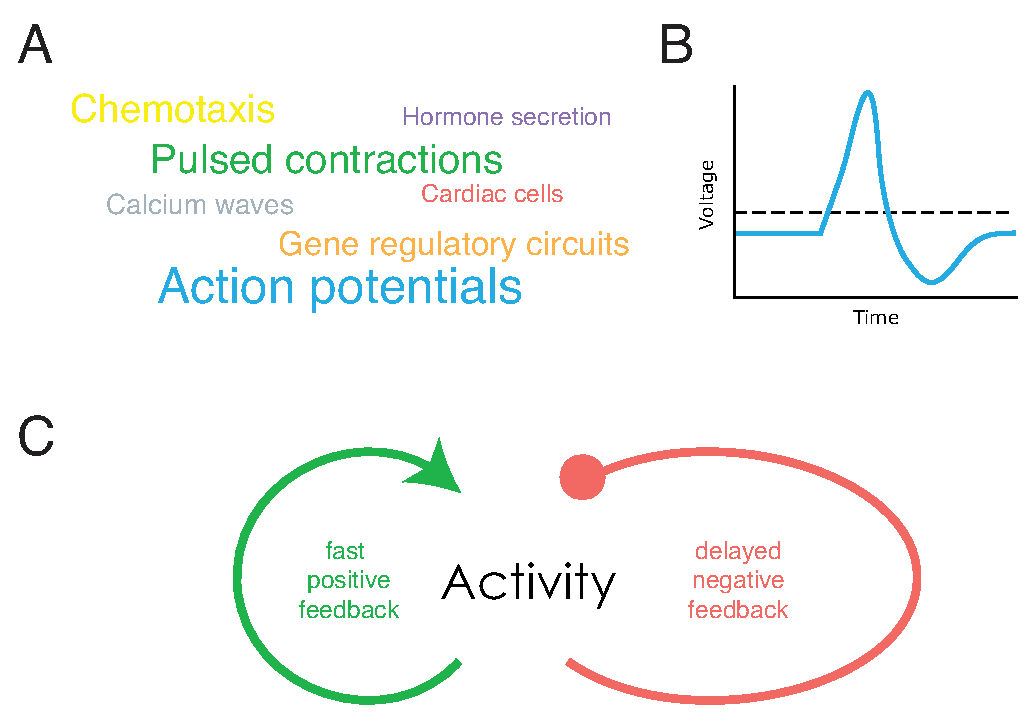
\includegraphics[width=1\textwidth]{Figure1-3}
\captionof{figure}[Pulsed contractions are an excitable system.]{\textbf{Pulsed contractions are an excitable system.} (A) Word cloud of well-known biological phenomena that are thought exhibit excitable dynamics. (B) Example of an action potential. (C) Simple feedback circuit diagram illustrating the two key requirements for excitable dynamics: fast positive feedback and delayed negative feedack.}
\end{figure}




\subsection{Contractile Instability Model}
%Introduction the contractile instability model, Turing, Meinhardt
The mathematical analysis of spontaneous pattern formation during morphogenesis has been extensively studied since Alan Turing published his seminal paper in 1952 \cite{Turing:1952vn, Kondo:2010bx}.  Turing proposed that a system of morphogens that are reacting and diffusing  is sufficient to drive spatial patterning within biological tissues.  His key insight was that diffusion could destabilize the steady state of a system of reacting chemicals.  This insight was counterintuitive, as diffusion can be thought to dampen spatial heterogeneities.  In the paper, Turing described a reaction-diffusion mechanism in which an activator species diffused slowly, while an inhibitor species diffused more rapidly.  Based on their differential diffusivities, and mutual interactions, Turing showed that a small spatial perturbation can destabilize the activator-inhibitor system at steady state.  The small perturbation is amplified over time, leading to a new steady state where the concentration of each species varies with position.  This mechanism is an example of diffusion-driven instability \cite{Segel:1972wb}.

Gierer and Meinhardt, and independently Segel and Jackson, extended Turing's reaction-diffusion system of morphogens into a more general class of models \cite{Gierer:1972vq,Segel:1972wb}.  Their mathematical analysis confirmed that there are two features that play a central role in pattern formation: \textit{local autocatalytic activation of the activator} and \textit{long-range inhibition by the inhibitor}.  The activator is autocatalytic if a small increase in its concentration/activity promotes a further increase in concentration/activity.  In general, the autocatalysis does not have to be direct and could instead be mediated by other factors that have been abstracted away in the model.  Autocatalysis alone is not sufficient to generate spatial patterns. Once the activator starts to increase, positive feedback would lead to global activation.  Thus in order for spatial patterns to form, autocatalysis of the activator must be modulated by long-range inhibition by a rapidly-diffusing inhibitor.  


%Figure 1.4
\begin{figure}[!htbp]
\centering
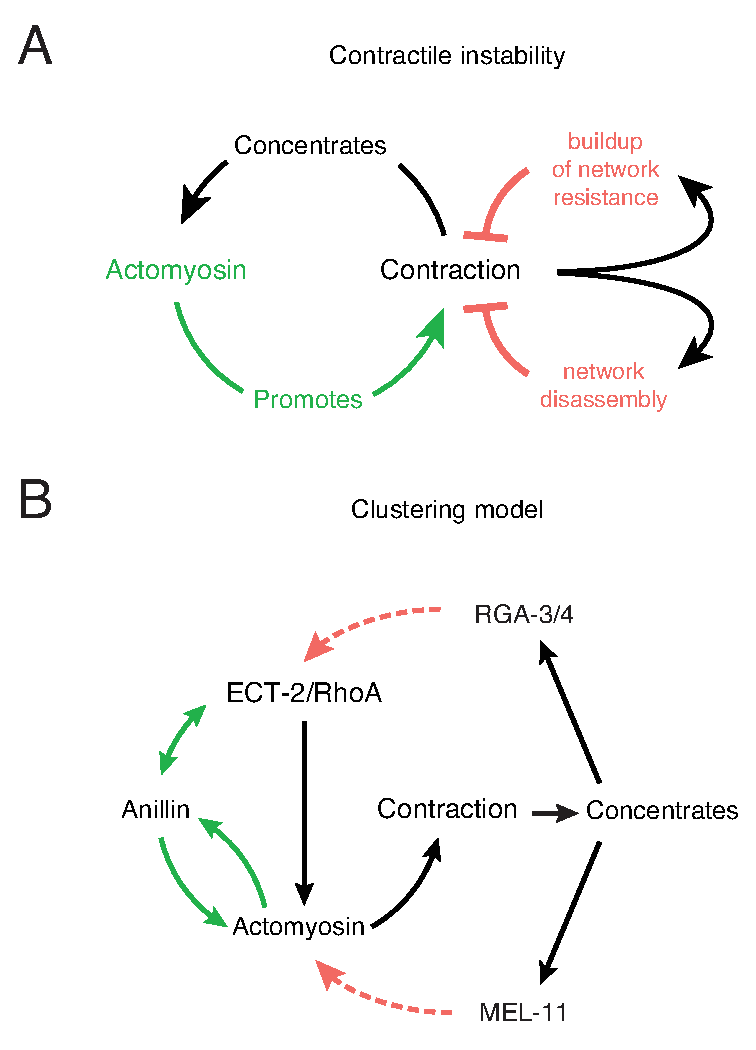
\includegraphics[width=0.85\textwidth]{Figure1-4}
\captionof{figure}[Potential feedback mechanisms governing the initiation and termination of pulsed contractions.]{\textbf{Potential feedback mechanisms governing the initiation and termination of pulsed contractions.} (A) \textbf{Contractile instability model:} Local Myosin II contractility concentrates F-actin, Myosin II, and/or their upstream regulators.  Network disassembly or a build up of network resistance can negatively feedback to inhibit contractility. (B) \textbf{Clustering model:} Anillin-mediated positive feedback clusters contractile components by mediating mutual binding interactions between F-actin, Myosin II, and or ECT-2/RhoA.  Delayed inhibition of RhoA or Myosin II is one potential form of delayed negative feedback in the system.}
\end{figure}



Although Turing noted the importance of mechanics in morphogenesis, his reaction-diffusion model did not take into account the mechanical properties of living tissues \cite{Howard:2011da}.  We now know that forces generated by the actomyosin cytoskeleton play an important role in tissue morphogenesis.  In terms of mechanical properties, the cytoskeleton can be thought of as an active fluid \cite{Kruse:2004il}.  Actomyosin networks continually consume energy, and have fluid-like properties that depend on the length, stability, and cross-linking of actin filaments \cite{Kruse:2004il}.  Bois \textit{et al.} developed a mathematical model of pattern formation of the cortex in which they model the cytoskeleton as an active fluid \cite{Kruse:2004il, Bois:2011kx}.  Although their mathematical analysis was similar to that of Turing and others, Bois \textit{et al.} departed conceptually from older models by considering advection-driven instability \cite{Turing:1952vn,Gierer:1972vq,Segel:1972wb,Bois:2011kx}.  They showed analytically that a single chemical species that obeys certain reaction-diffusion-advection equations is capable of generating spatial patterns.  In their model, it is essential that local force generation is proportional to the concentration of the chemical species.  As a result, their model recapitulates the local activation and lateral inhibition properties proposed by Gierer and Meinhardt \cite{Gierer:1972vq}.  Positive feedback in this model occurs when a local increase in the concentration of the activator promotes a further increase in concentration due to advection (Figure 1.4A).  Lateral inhibition occurs when neighboring regions of the cortex are depleted of the activator.  Interestingly, Bois \textit{et al.} showed that their model is capable of generating patterns in the absence of chemical reactions \cite{Bois:2011kx}.  Later work from the same group showed that by including reaction terms, their simulations could generate pulsatile patterns that are reminiscent of Myosin II pulses observed animal cells \cite{Kumar:2014ux, Munro:2004jk}.  Simulations from the Munro lab suggest that network disassembly, or a build up of network resistance, can provide delayed negative feedback in terminating pulsed contractions (personal communication).


%\subsection{Tension-based myosin accumulation}


\subsection{Clustering Models}
Another model that could explain pulsed contractility is a clustering model in which a scaffold protein promotes the accumulation of factors important for pulsed contractions.  Anillin is a scaffold protein that was first identified as an F-actin bundling protein in \textit{Drosophila} \cite{Miller:1989vn}.  Later work showed that Anillin also binds Myosin II \cite{Piekny:2010es,Zhang:2010fb}.  In the most general form of the clustering model, Anillin could promote pulsed contractions by mediating mutual interactions between factors such as RhoA, Ect2, Myosin II, and F-actin.   Maddox \textit{et al.} proposed a similar model to explain pulsed contractions in the early \textit{C.elegans} embryo \cite{Maddox:2005gd}.  Under wild-type conditions, \textit{C.elegans} embryos exhibit membrane ruffling in which deep membrane invaginations correspond to pulsed contractions (\cite{Maddox:2005gd}, see Chapter 2).  Maddox \textit{et al.} showed that \textit{C.elegans} embryos that have been strongly depleted of Anillin fail to ruffle \cite{Maddox:2005gd}.  They also showed that Myosin II failed to accumulate robustly in cortical patches when Anillin was depleted \cite{Maddox:2005gd}.  Instead, Myosin II localized uniformly on the cortex.  Furthermore, Anillin formed cortical patches that appeared to have roughly the same size in spacing as wild-type patches in the absence of Myosin II \cite{Maddox:2005gd}.  Maddox \textit{et al.} proposed a model in which local clusters of anillin, independent of Myosin II-dependent contractility, promote pulsed contractions by locally recruiting F-actin and Myosin II.  In this model, positive feedback between anillin and F-actin drives the accumulation of other factors such as Myosin II and septin.


%Anillin could mediates RhoA recruitment
In an alternate clustering model, Anillin-mediated autocatalytic activation of RhoA could recruit Myosin II and F-actin to pulsed contractions (Figure 1.4B).  Piekny \textit{et al.} provided evidence that suggested that RhoA and Anillin might regulate each other's localization to the cytokinetic furrow in dividing HeLa cells \cite{Piekny:2008jf}.  They showed that Anillin failed to localize to the furrow in the absence of RhoA, and that Anillin stabilizes RhoA in fixed cells \cite{Piekny:2008jf}.  They also showed that human Anillin contains a conserved C-terminal domain (called the Anillin homology domain) that is required for Anillin to function and localize properly \cite{Piekny:2008jf}.  They also showed that the Anillin homology domain binds active RhoA.  Later work by Frenette \textit{et al.} showed that the Anillin homology domain interacts with the PH domain of human Ect2 during cytokinesis \cite{Frenette:2012do}.  Furthermore, recent work by Manukyan \textit{et al.} showed that overexpressing Anillin in HeLa cells leads to an increase in RhoA activation \cite{Manukyan:2015gg}.  Taken together, these results suggest a mechanism whereby Anillin could promote autocatalytic activation of RhoA, and hence pulsed contractions, by locally mediating interactions between RhoA and Ect2 on the cortex.  


Since Anillin is a scaffold protein, it could mediate the initiation of pulsed contractions through multiple parallel pathways.  For example, in addition to promoting RhoA auto-activation, Anillin  could also promote contractile instability by stabilizing interactions between Myosin II and F-actin.  Support for this model comes from experiments where Piekney \textit{et al.} showed that Anillin stabilizes Myosin II at the furrow during cytokinesis \cite{Piekny:2008jf}.  Furthermore, Maddox \textit{et al.} showed that although depletion of Anillin led to a strong decrease in the amplitude and duration of Myosin II pulses in \textit{C.elegans} embryos, weak Myosin II pulses still formed on the cortex.



\section{My work}
%Pulsed contractions are ubiquitous
Much of what we know about how pulsed contractions are regulated, and what we can surmise about their functional importance, has come from studies in \textit{Drosophila} where they have been implicated in tissue invagination, tissue elongation, tissue closure, and wound healing \cite{Martin:2009du,Rauzi:2010fs, Solon:2009hg, Razzell:2014eb}.   However, pulsed contractions have also been documented in other organisms.  For example, early studies have documented pulsed contractions during polarization in early \textit{C. elegans} embryos and convergence extension in \textit{Xenopus}  \cite{Munro:2004jk, He:2010gf}.  More recent studies have shown that pulsed contractions might also play an important role in driving shape changes during compaction in mouse embryos, as well as apical constriction during neural tube closure in \textit{Xenopus} \cite{Maitre:2015hc, Christodoulou:2015kb}. 

%Why study pulsed contractions
The fact that pulsed contractions are ubiquitous in higher eukaryotes suggests that they likely play important functional roles, even though those roles may not be immediately apparent.  One possibility is that pulsed contractions might provide a way for cells within tissues to rapidly sample different conformations as they change shape.  Another possibility is that pulsed contractions help to maintain tissue integrity during morphogenesis \cite{Vasquez:2014hv}.  For example, since apical constriction of ventral furrow cells is asynchronous, pulsatile shape changes might reduce tension within the tissue \cite{Martin:2009du, Vasquez:2014hv,Fischer:2014hm}.  Thus future experimental or theoretical studies might provide insight as to why \textit{Drosophila} embryos, for example, might prefer pulsed contractions over circumferential actin cables for driving apical constriction.  From a more general perspective, pulsed contractions might belong to a broader class of mechanisms that include phenomena such as cell shape oscillations and wound healing \cite{Gorfinkiel:2016bv,Razzell:2014eb}.  From a more basic perspective, pulsed contractions are an interesting example of a complex self-organized contractile system.  Therefore, studying pulsed contractions might provide insight into the principles governing the assembly of actomyosin networks, as well as uncover general mechanisms that cells use to tune actomyosin networks to accomplish specific tasks.


%Outline my approach
How, then, are pulsed contractions initiated and terminated?  Which factors are required for pulsed contractions?  In what order are these factors recruited to pulsed contractions?  What determines the size and spatial organization pulsed contractions?  How might different organisms tune the activity of regulatory molecules and the assembly/disassembly kinetics of actomyosin in order to regulate the dynamics of pulsed contractions?  Previous experimental and theoretical research has given us a roadmap for answering these questions.  Building on these previous results, the purpose of this thesis is to provide insight into some of the unanswered questions, as well as provide a novel conceptual framework for guiding future experiments.  In the remainder of this chapter I will outline my general approach and provide a preview of chapters 2 and 3.  First, I will provide the rationale for using \textit{C. elegans} as a model system for pulsed contractility and introduce the relevant components.  Next, I will describe the experimental and modeling approach that my collaborators and I have taken to investigating pulsed contractions.  Last, I will describe the significance of the work we have done.


\subsection{\textit{C. elegans} as a model system for studying pulsed contractions}
Pulsed contractions were first identified in the \textit{C. elegans} where they occur during polarization in the zygote P0, during the first cell division, in the larger anterior daughter cell AB, and at the first stage of gastrulation (Figure 1.5) \cite{Munro:2004jk, RohJohnson:2012cf}.  Preliminary observations also suggest that pulsed contractions occur in the smaller posterior daughter cell P1 after the first cell division (data not shown).  Although we currently suspect that pulsed contractions do not play a significant functional role in \textit{C. elegans} development, there are many reasons that make the early embryo an excellent system to study actomyosin dynamics in general, and pulsed contractions in particular.  First, \textit{C. elegans} has a rapid generation time and is very easily cultured \cite{Jorgensen:2002ej}.  Second, the \textit{C. elegans} early embryo is large and optically clear, and the availability of many fluorescent markers makes it easy to acquire high quality images of the cortex with high spatial and temporal resolution.  Third, pulsed contractions in \textit{C. elegans} occur in both the single cell zygote P0 and the larger anterior daughter cell AB in the two cell stage (Figure 1.5).  P0 and AB are both large single cells, and the pulses are highly stereotyped within each context.  We can therefore compare and contrast pulses in P0 to pulses in AB in a quantitative manner by making reproducible measurements that have statistical significance.  For example, we can use cutting edge single-molecule techniques to measure the turnover and mobility of various components of the cortex \cite{Robin:2014jf}. 

%Figure 1.5
\begin{figure}[!htbp]
\centering
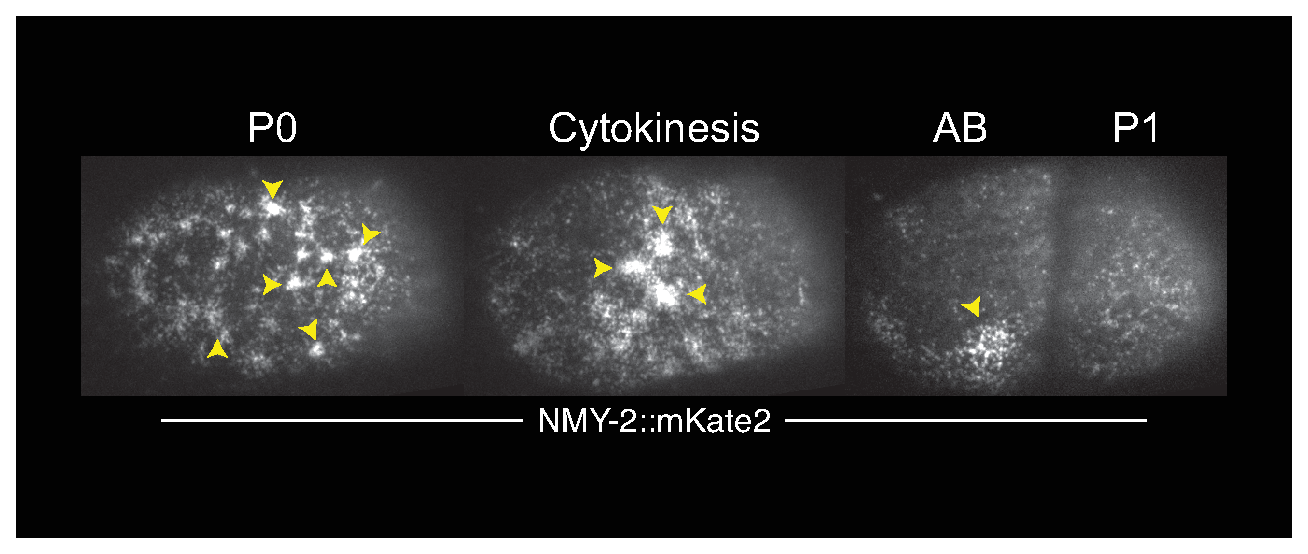
\includegraphics[width=0.85\textwidth]{Figure1-5}
\captionof{figure}[Pulsed contractions in the early \textit{C.elegans} embryo.]{\textbf{Pulsed contractions in the early \textit{C.elegans} embryo.} Micrographs of a representative \textit{C.elegans} embryo expressing NMY-2::mKate2 during the 1-cell stage, cytokinesis, and 2-cell stage.  Yellow arrowheads indicate pulsed contractions.}
\end{figure}

%Genetics as a tool
Another compelling reason for using the \textit{C. elegans} embryo as a model system is due to its history as a classic model organism.  As such, we know a great deal about \textit{C. elegans} genetics \cite{Jorgensen:2002ej}.  Large-scale mutagenesis screens, like the original screen by Sydney Brenner, have identified numerous mutant phenotypes \cite{Brenner:1974wn}.  Similarly, RNA interference (RNAi), either by feeding or injection, has also been used to conduct large-scale screens \cite{Timmons:2001wg, Kamath:2003bk}.  A recent RNAi  screen by Fietvet \textit{et al.} has identified important regulators of cell polarity and actomyosin contractility in \textit{C. elegans} \cite{Fievet:2013ho}.  RNAi treatment can be used on a more fine scale to gradually deplete the concentration of a protein \textit{in vivo}.  This gives researchers the ability to assay protein function over a range of concentrations. 


Knowledge of \textit{C. elegans} genetics has also helped researchers develop tools for generating fluorescent proteins.  For example, the development of methods for inserting single-copy transgenes in the worm genome has allowed researchers to make transgenic lines that stably express important fluorescent markers such as the now famous active RhoA biosensor (GFP::AHPH) \cite{FrokjaerJensen:2008kj, Tse:2012fp}.  When the fluorescent protein of interest is expressed on top of the wild-type protein, RNAi can be used to specifically target the fluorescent probe.  This gives researchers the ability to study the single molecule dynamics of their protein of interest in a wild type background \cite{Robin:2014jf}.  More recent and exciting methods have been developed to use the CRISPR/Cas9 system to edit the genome.  These tools now give researchers the ability to fluorescently tag proteins at their endogenous locus \cite{Hsu:2014ck}.  This method, which has largely been pioneered in \textit{C. elegans} by Daniel Dickinson in the Goldstein lab, can now be used to create fully labeled and fully functional fluorescent proteins \cite{Dickinson:2013ea, Dickinson:2016cv}.  Thus, the advantages of using the \textit{C.elegans} early embryo make it easy to image, quantify, manipulate, and compare actomyosin dynamics in order to elucidate the mechanisms underlying pulsed contractions.  


\subsection{The key components}
%Myosin
There are many signaling molecules and actin binding proteins that regulate the structure and dynamics of cortical actomyosin networks (see Section 1.2 for a brief overview).  Recent experiments have identified which of these components might constitute a pulsed contractility module, i.e., a core set of interacting proteins whose activity is sufficient for the formation of pulsed contractions.  F-actin and Myosin II, the main force generating molecules, were shown to strongly co-localize in fixed P0 embryos during late meiosis \cite{Munro:2004jk}.  Myosin II activity is likely under the control of Rho-binding kinase (LET-502) and myosin phosphatase (MEL-11).  Piekny \textit{et al.} showed that by inhibiting LET-502 activity by combining \textit{let-502} mutants and \textit{let-502} RNAi, embryos failed to form robust furrows during pseudocleavage and cytokinesis \cite{Piekny:2002vx}.  They also showed that \textit{mel-11} mutants ingressed furrows faster, and formed ectopic furrows \cite{Piekny:2002vx}.  These experiments suggest that LET-502 and MEL-11 have antagonistic effects on myosin II behavior during furrow ingression.  Thus, LET-502 appears to promote contractility in the early embryo, while MEL-11 inhibits it. 


%Actin ,CYK-1, PFN-1, ARX-2 UNC-60, Anillin
CYK-1 is a major \textit{C. elegans} formin that is homologous to Dia in \textit{Drosophila}.  Together with profilin (PFN-1 in \textit{C. elegans}), CYK-1 has been shown to be an important regulator of contractile ring assembly \cite{Severson:2002ve}.  Severseon \textit{et al.} showed that depletion of PFN-1 or CYK-1 prevents furrow formation during pseudocleavage and cytokinesis.  These results suggest that PFN-1 and CYK-1 are likely regulators of pulsed contractions, as pulsed contractions occur around the same time.  Similarly, cofilin (UNC-60 in \textit{C. elegans}) which is an important regulator of actin turnover, was also shown to be important for early embryonic development \cite{Ono:2003bg}.  While ARP-2/3 (ARX-2 and ARX-3 in \textit{C. elegans}) likely assembles branched filaments on the cortex, Severson \textit{et al.} showed that ARP-2/3 is not required for polarization or cytokinesis.  Thus, it seems possible that ARP-2/3 might regulate the dynamics of pulsed contractions, but not their formation.  Other classes of proteins that might regulate pulsed contractions via their effect on actin structure and dynamics include cross-linking and bundling proteins.  The scaffold protein Anillin (ANI-1 in \textit{C. elegans}) was first identified as an F-actin bundling protein in \textit{Drosophila} \cite{Field:1995vb}.  Experiments by Maddox \textit{et al.} showed that depleting ANI-1 resulted in a strong reduction of myosin II within cortical patches (i.e., pulsed contractions).  This suggests that ANI-1 might play a role in facilitating force generation within pulsed contractions by stabilizing Myosin II on actin filaments.




%Regulators: Activation of RhoA, ECT-2, NOP-1, RGA-¾ (Motegi, Tse)
The RhoA (RHO-1 in \textit{C.elegans} signaling pathway has been shown to regulate cortical actomyosin dynamics in the early \textit{C.elegans} embryo \cite{Motegi:2006hi, Tse:2012fp}.  Motegi \textit{et al.} showed that partial depletion of RhoA, or its GET ECT-2, eliminates cortical flows, pseudocleavage furrow formation, and polarity establishment in the zygote P0 \cite{Motegi:2006hi}.  Similarly, Jenkins \textit{et al.} demonstrated that P0 embryos expressing NMY-2::GFP no longer form pulsed contractions when RhoA or ECT-2 is partially depleted \cite{Jenkins:2006cb}.  Later work by Tse \textit{et al.} identified a novel protein, NOP-1, whose activity also controls RhoA activation during polarization and cytokinesis \cite{Tse:2012fp}. Similar to \textit{ect-2} RNAi or mutant embryos, \textit{nop-1} mutants do not form pseudocleavage furrows, and in many cases lack cortical flows \cite{Tse:2012fp}.  While \textit{nop-1} mutants undergo cytokinesis, embryos strongly depleted of ECT-2 do not.  Since this result suggests that NOP-1-mediated contractility requires ECT-2, the authors argue that NOP-1 likely functions upstream of ECT-2 in promoting RhoA activation \cite{Tse:2012fp}.  They also observed that \textit{nop-1} mutants do not form dense Myosin II or Anillin foci during polarity establishment \cite{Tse:2012fp}.  The localization pattern of an active RhoA biosensor (GFP::AHPH) suggests that active RhoA also accumulates within contractile foci \cite{Tse:2012fp}.  Consistent with this idea, they observed a loss of cortical active RhoA in \textit{nop-1} mutants.  Taken together, these results suggest that ECT-2/NOP-1-mediated activation of RhoA is important for the formation of pulsed contractions.




%Inactivation of RhoA by RGA-3/4 (Schoenegg, Smutz)
The redundantly acting Rho GAPs RGA-3 and RGA-4 are the primary GAPs that inhibit RhoA activation during polarization \cite{Schmutz:2007jq, Schonegg:2007if}.  RGA-3 and RGA-4 (RGA-3/4) were first identified in an RNAi screen for regulators of cortical contractility \cite{Schmutz:2007jq}.  Unlike \textit{ect-2} and \textit{nop-1} mutants, \textit{rga-3/4} RNAi embryos are hypercontractile \cite{Schmutz:2007jq, Schonegg:2007if}.  Consistent with RGA-3/4 acting in a pathway with RhoA, co-depletion of RhoA and RGA-3/4 rescues the hypercontractility phenotype \cite{Schmutz:2007jq, Schonegg:2007if}.  Schonegg \textit{et al.} confirmed that the RGA-3 and RGA-4 GAP domains enhance RhoA GTPase activity \textit{in vitro} \cite{Schonegg:2007if}.  Tse \textit{et al.} showed that depleting RGA-3/4 led to an increase in the active RhoA biosensor on the cortex during cytokinesis \cite{Tse:2012fp}.  Similarly, cortical NMY-2::GFP levels increased in \textit{rga-¾} RNAi embryos \cite{Schonegg:2007if}.  A fluorescent RGA-3 transgene (YFP::RGA-3) localized to cortical foci in pattern consistent with its accumulation in pulsed contractions.  Like NMY-2::GFP, YFP::RGA-3 foci also flowed anteriorly during polarity establishment  \cite{Schonegg:2007if}.  Thus, active RhoA-mediated control of pulsed contractions appears to be regulated antagonistically by ECT-2 and RGA-3/4.

\subsection{Overview of experimental approach}
%Microscopy and image analysis
In this thesis, my collaborators and I have used a combination of live-cell imaging, quantitative image analysis, genetic and pharmacological perturbations, and mathematical modeling to investigate the mechanisms underlying pulsed contractions.  We used single- and dual-color near-total internal reflection (TIRF) microscopy to image the cortex of live \textit{C. elegans} embryos in the one- and two-cell stage.  In contrast to conventional spinning disk microscopy, near-TIRF illuminates a thin slice of the embryo near the coverslip.  This enhances the fluorescence signal of the plane of illumination versus that of the background, and limits photobleaching.  Near-TIRF microscopy is also amenable to fast image acquisition for high temporal resolution.  By imaging two fluorescent proteins, we have co-monitored various pairs of proteins during pulsed contractions to assay their dynamics over time.  We have extended this methodology to include various genetic perturbations such as RNAi and the use of mutants.  The procedure we use to mount live specimens allows us to combine chronic or acute drug treatments with high quality imaging.  Finally, mathematical modeling has allowed us to abstract away unnecessary details and focus on the most salient features of pulsed contractility in order to recapitulate their dynamics \textit{in silico}.

%Figure 1.6
\begin{figure}[!htbp]
\centering
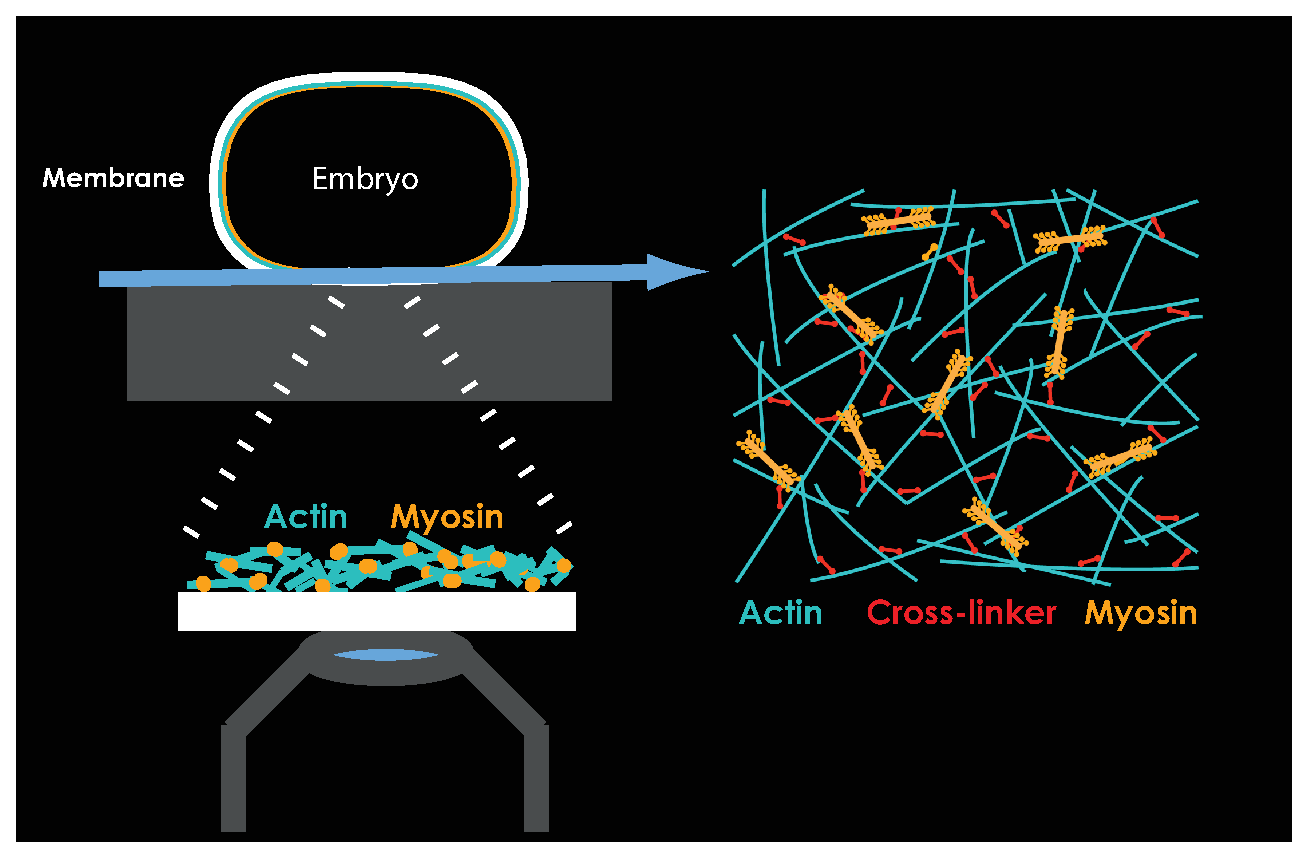
\includegraphics[width=0.85\textwidth]{Figure1-6}
\captionof{figure}[Schematic of experimental setup.]{\textbf{Schematic of experimental setup.} The cortex of 1 and 2-cell embryos was imaged using two-color near-TIRF microscopy.}
\end{figure}

\subsection{The significance of this thesis} 
The work presented in this thesis represents a significant contribution to our understanding of pulsed contractions.  We have identified what we believe constitutes a core set of proteins regulating pulsed contractions in \textit{C. elegans}.  Our experiments have demonstrated that pulsed contractions in \textit{C. elegans} are not primarily initiated by a contractile instability or clustering mechanism.  Instead, we have demonstrated that local activation and inactivation of RhoA regulates the initiation and termination pulsed contractions independent of myosin II-dependent contractility (see Chapter 2).  Further experiments demonstrate that tuning various effectors downstream of RhoA has a profound impact on actomyosin contractility as well as RhoA spatial dynamics (see Chapter 3).  The combination of these results suggest that RhoA spatial patterning is tightly coupled to cortical actomyosin contractility.  To explain these results, we describe a novel conceptual framework in which pulsed contractions are represented by an activator-inhibitor system in which the individual components undergo reactions, diffusion, and advections.  Coupling the inhibitor to the actomyosin cortex potentiates mechanical feedback onto RhoA  (see Chapter 4).  This novel framework has been synthesized from our own experiments, as well as important experimental and theoretical results from the Martin, Glotzer, Bement, and Grill groups.  We expect the results and ideas presented here to guide future investigations of pulsed contractions in particular, and other biological processes governed by mechanical regulation of RhoA in general (see Chapter 4).






\end{document}
					 				
			
		




\documentclass{ucetd}
\usepackage{subfigure,epsfig,amsfonts}
\usepackage{natbib}
\usepackage{amsmath}
\usepackage{amssymb}
\usepackage{amsthm}
\graphicspath{ {figures/ch2/} }
\begin{document}

\chapter{Excitable RhoA dynamics drive pulsed contractions in the early C. elegans embryo}

\section{Preface}
This chapter has been submitted to the BioRxiv preprint server with the following citation: Robin FB, Michaux JB*, McFadden W, Munro EM.  Excitable RhoA dynamics drive pulsed contractions in the early C. elegans embryo.  BioRxiv (2016) Published online September 21, 2016. http://dx.doi.org/10.1101/076356.


This work was done in collaboration with Fran\c{c}ois Robin and William McFadden in Edwin Munro's lab at the University of Chicago.  Fran\c{c}ois performed the single-molecule imaging experiments, particle tracking, and statistical analyses documented in Figures 2.2, 2.3, 2.10, and 2.11.  William used MATLAB to create a mathematical model.  This model, which was constrained by my experimental measurements, is documented in Figure 2.9 and section 2.5 (Chapter 2 Materials and Methods).

\section{Abstract}
Pulsed actomyosin contractility underlies diverse modes of tissue morphogenesis, but the mechanisms that generate pulsed contractions are still poorly understood.  Here, we combine quantitative imaging with genetic perturbations and mathematical modeling to identify a core mechanism for pulsed contractility in early \textit{C.elegans} embryos.  We show that pulsed accumulation of actomyosin is governed almost entirely by local control of assembly and disassembly downstream of RhoA.  Pulsed activation and inactivation of RhoA precedes, respectively, the accumulation and disappearance of actomyosin, and persists in the near complete absence of Myosin II.  Autocatalytic activation of RhoA underlies rapid pulse initiation, while delayed accumulation of the RhoA GTPase activating proteins (GAPs) RGA-3/4 provides negative feedback to terminate each pulse. Mathematical models, tightly constrained by our experiments, confirm that this combination of positive and negative feedback is sufficient to generate locally pulsatile RhoA dynamics and reproduce the observed waveform of RhoA activation and RGA-3/4 acumulation. We propose that excitable RhoA dynamics are a common driver for pulsed contractility that can be tuned or coupled to actomyosin dynamics in different ways to produce a diversity of morphogenetic outcomes.


\section{Introduction}
Pulsed contractility is a widespread mode of actomyosin contractility expressed by many non-muscle cells in which transient accumulations of F-actin and Myosin II accompany local contractions of the cell surface. Pulsed contractions were first identified in the polarizing \textit{C.elegans} zygote \cite{Munro:2004jk}, and have now been documented in a wide variety of embryonic and extra-embryonic epithelia \cite{He:2010gf, Blanchard:2010kt, Rauzi:2010fs, David:2010bt, Martin:2009du, Solon:2009hg} and mesenchymal cells \cite{Kim:2011cc}. A similar phenomenon known as cell shape oscillations have been observed in many cultured cells \cite{Sedzinski:2011ef, Salbreux:2007fc, Kapustina:2008ds}. Pulsed contractions produce transient shape changes that can be biased or rectified in different ways to produce distinct morphogenetic outcomes such as tissue invagination \cite{Martin:2009du}, tissue elongation \cite{Rauzi:2010fs, Levayer:2013el, He:2010gf}, epithelial tissue closure \cite{Solon:2009hg} and wound healing \cite{Razzell:2014eb}. During embryonic development, pulsed contractions may represent an adaptation to accommodate rapid cell and tissue deformations while maintaining overall tissue integrity \cite{Vasquez:2014hv}. In other contexts, such as in many cultured cells, shape oscillations may represent an aberrant behavior that manifests when cells lose normal adhesion to their substrates \cite{Salbreux:2007fc, Paluch:2005da}, or when microtubules are depolymerized \cite{Kapustina:2013gc, Kapustina:2008ds, Rankin:2010je, Werner:2007bx, Piekny:2008jf, Bornens:1989wc} or when contractile tension is very high during cytokinesis \cite{Sedzinski:2011ef}.

Despite their widespread occurrence and increasing evidence for their functional relevance, the mechanisms that initiate and terminate pulsed contractions remain poorly understood. From a dynamical perspective, pulsed contractions represent a form of excitable behavior, exemplified by action potentials in neuronal cells \cite{Izhikevich:2007aa} or pulses of intracellular calcium release observed in many cell types \cite{Goldbeter:1996aa}.  Theoretical studies highlight two key ingredients for excitability: positive feedback to drive rapid upswing in activity, and delayed negative feedback to bring it back down again. A key challenge is to identify the specific modes of positive and negative feedback that drive pulsed contractions.

Multiple forms of positive feedback could contribute to initiating pulsed contractions. For example, local actomyosin-based  contraction could promote further accumulation of actomyosin through mechanosensitive motor-filament binding \cite{He:2010gf, FernandezGonzalez:2009hp,Ren:2009ep, Effler:2006hc, Schiffhauer:2016iy}, by enhancing actin filament assembly and/or stability \cite{Hayakawa:2011dq, DeLaCruz:2015dj}, or by transporting and concentrating actomyosin and/or its upstream activators \cite{Munjal:2015bx, Dierkes:2014tm}. Alternatively, dynamic clustering of F-actin and/or Myosin II by scaffolding proteins such as Anillin could promote Myosin II recruitment and focal contraction \cite{Maddox:2005gd}. Finally, autocatalytic activation of upstream regulators such as RhoA could drive local excitation, independent of, or in addition to, myosin-based tension or network contraction \cite{Zhang:2015bx, Munjal:2015bx, Bement:2015jp}. Similarly, multiple forms of delayed negative feedback could contribute to terminating pulses, including progressive buildup of steric or elastic resistance to further contraction \cite{Dierkes:2014tm}, or contraction-mediated disassembly, or delayed recruitment of disassembly factors or inhibitors of Myosin II or RhoA \cite{Munjal:2015bx, Kasza:2011ft, Bement:2015jp}.   

Here we combine quantitative imaging with experimental manipulations and mathematical modeling to identify the dynamical basis for pulsed contractility in the early \textit{C.elegans} embryo. Using single-molecule imaging and particle tracking analysis, we provide definite evidence that the initiation of pulsed contractions does not involve or require local redistribution of actomyosin or its upstream activators.  Instead, pulsed contractions are driven by local pulses of RhoA activity, which feed forward to control local accumulation of downstream targets F-actin, Myosin II and Anillin. We present evidence that pulsed accumulation of RhoA is governed by locally excitable RhoA dynamics: local autocatalytic activation of RhoA drives the rapid upswing of RhoA activity during pulse initiation, while F-actin-dependent recruitment of the redundantly acting RhoA GTPase activating proteins (GAPs) RGA-3/4 provide delayed negative feedback to terminate the pulse.  A minimal model, sharply constrained by our experimental data, suggests that this combination of feedback is sufficient to generate locally excitable or oscillatory RhoA dynamics and to explain quantitatively the temporal dynamics of RhoA activation and RGA-3/4 accumulation during each pulse. We propose that excitable RhoA dynamics defines a core mechanism for pulsed contractility and suggest that this mechanism may be tuned or filtered through downstream effectors to control the size or spacing or lifetime of pulsed contractions.  

\section{Results}
Pulsed contractions were originally described in \textit{C.elegans} during interphase in the polarizing zygote P0 (Figure 2.2.1A-C, individual pulses indicated by white arrowheads in Figure 2.2.1B; \cite{Munro:2004jk}). In these cells, pulsed contractions are associated with transient deep invaginations of the cell surface (magenta arrows in Figure 2.2.1A,B); this makes it more difficult to quantify local changes in density of cortical factors during individual pulses, because these measurements could be confounded by movements of the cortex in/out of the plane of focus. Therefore, we focused on pulsed contractions that occur at the two-cell stage in the anterior blastomere known as AB (Figure 2.2.1D-F, individual pulses indicated by white arrowheads in Figure 2.2.1E).  As in P0, pulsed contractions in AB involve transient accumulations of F-actin and Myosin II; they are associated with transient local contractions of the actomyosin cortex (Figure 2.2.1F), but they are not associated with pronounced invaginations of the cell surface. 

%Figure 2.2.1
\begin{figure}[!htbp]
\centering
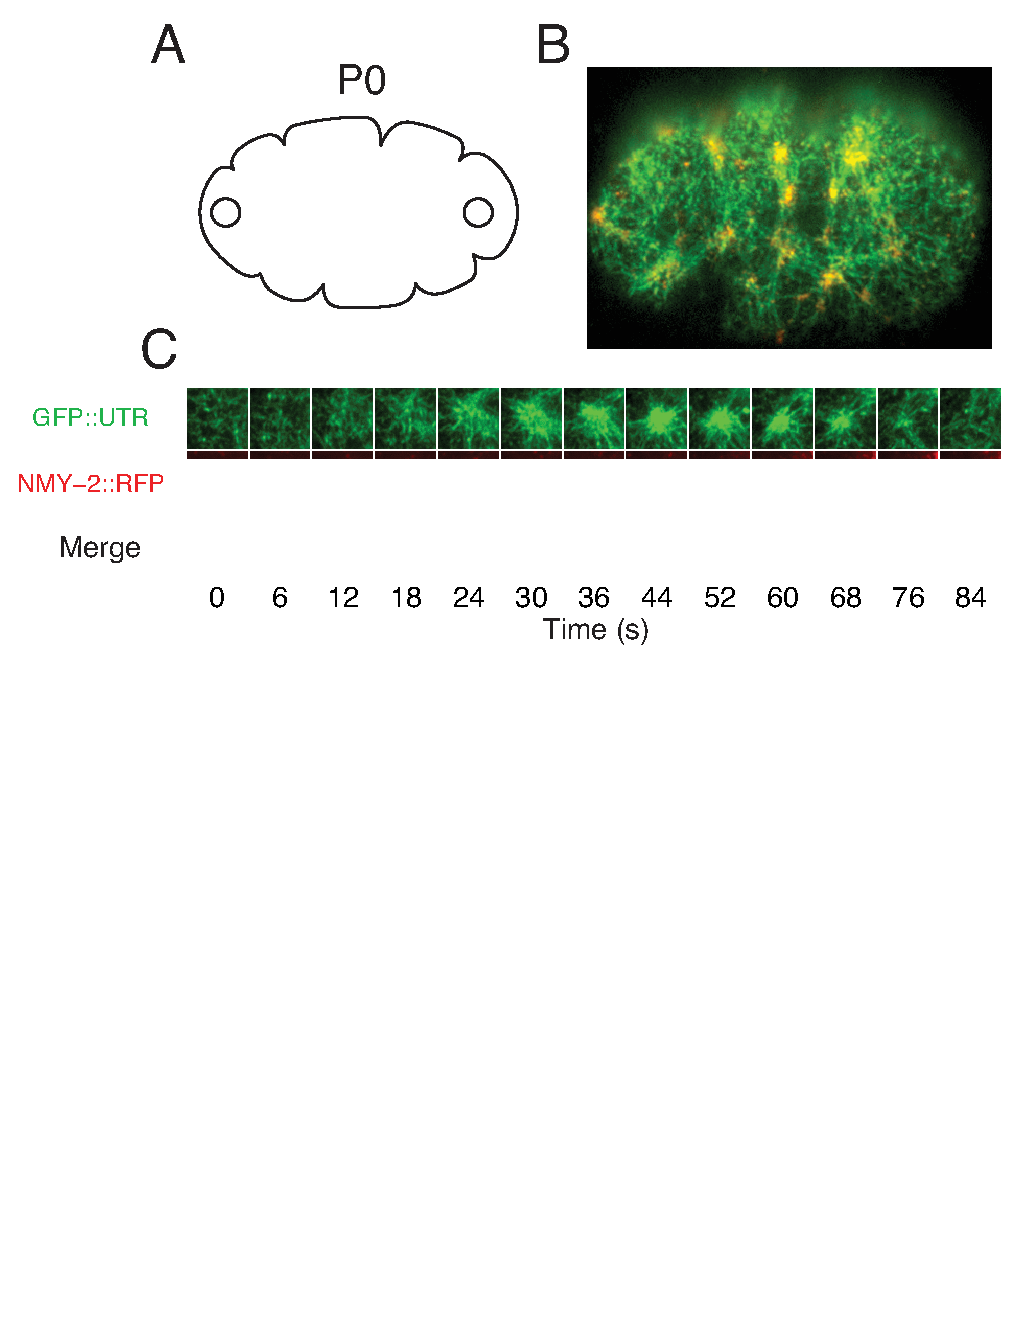
\includegraphics[width=0.85\textwidth]{Figure2-1}
\captionof{figure}[Actomyosin pulses in 1 and 2-cell stage embryos.]{\textbf{Actomyosin pulses in 1 and 2-cell stage embryos.} (A) Schematic view of the zygote P0 during early interphase.  Open circles represent the two pronuclei. (B) Micrograph of P0 in early interphase expressing GFP::UTR and NMY-2::RFP. In (A) and (B), white arrowheads indicate individual pulses and magenta arrows indicate membrane invaginations (ruffles). (C) Time evolution of a single pulse in P0. The square region measures $\sim$6.4$\mu$m by 6.4$\mu$m.  The time delay between frames is 6s for the first 6 frames, and 8s thereafter. (D) Schematic of an embryo at the early 2-cell stage, showing the anterior blastomere AB and the posterior blastomere P1.  Open circles represent the interphase nuclei. (E) Micrograph of an early two-cell stage embryo expressing GFP::UTR and NMY-2::RFP. White arrowheads indicate individual pulses (F) Time evolution of a single pulse. The square region measures $\sim$ 6.4$\mu$m by 6.4$\mu$m.  The time delay between frames is 2s for the first 5 frames, and 4s thereafter.}
\end{figure}


\subsection{Single-molecule analysis of actomyosin dynamics during pulsed contractions}
As a key step towards distinguishing different mechanisms for pulsed contractions, we used single-molecule imaging and single-particle tracking analysis to quantify the relative contributions of local turnover and redistribution to changes in F-actin and Myosin II density during individual pulses. As described previously \cite{Robin:2014jf}, we used RNAi against GFP to obtain embryos expressing single molecule levels of Actin::GFP or of the non-muscle myosin heavy chain fused to GFP (NMY-2::GFP) over the endogenous proteins (Figure 2.2.2A). We combined near-total internal reflection fluorescence (TIRF) imaging with single-molecule detection and tracking to measure the appearance, motion and disappearance of single-molecule speckles (Figure 2.2.2A-C, \cite{Robin:2014jf}). We assumed, with others \cite{Watanabe:2002jb, Vallotton:2004kz}, that single molecule appearance and disappearance events report directly on local rates of filament assembly and disassembly.  We have shown previously that rates of turnover measured by single-molecule tracking agree well with those measured from single-molecule data by fitting kinetic models to photobleaching curves  (\cite{Robin:2014jf}, Materials and Methods).

We then devised new methods to measure simultaneously: (a) single molecule appearance rates, disappearance rates and densities, and (b) local rates of cortical deformation, on a moving and deforming patch of cortex during individual pulsed contractions (Figure 2.10; see Materials and Methods for details). Briefly, we identified a reference frame for each pulse near the onset of contraction; within that frame, we identified a polygonal region of interest containing the contracting patch (dashed blue polygon in Figure 2.2.2A; hereafter “the patch”); we propagated the patch forward and backwards in time by extrapolating the displacements of tracked particles on or near its boundary (Figure 2.2D, Figure 2.10).   We then measured local deformation of the patch as frame-to frame changes in patch area, or by estimating a local strain rate from frame-to-frame displacements of the individual particles, with similar results in both cases (Figure 2.2E; Figure 2.11A-C; Materials and Methods).  At the same time, we measured the number of molecules and single-molecule appearance and disappearance rates within the patch over time (Figure 2.2F-H). Finally, we aligned single-molecule measurements with respect to the onset or termination of individual contractions to produce a dynamical signature of actin assembly, disassembly and deformation over the lifetime of a pulse (Figure 2.3A-D; Figure 2.11D-F). These measurements allowed us to distinguish, cleanly, changes in single-molecule densities due to local assembly and disassembly from those due to local contraction (or expansion) of the cortical patch.


%Figure 2.2.2
\begin{figure}[!htbp]
\centering
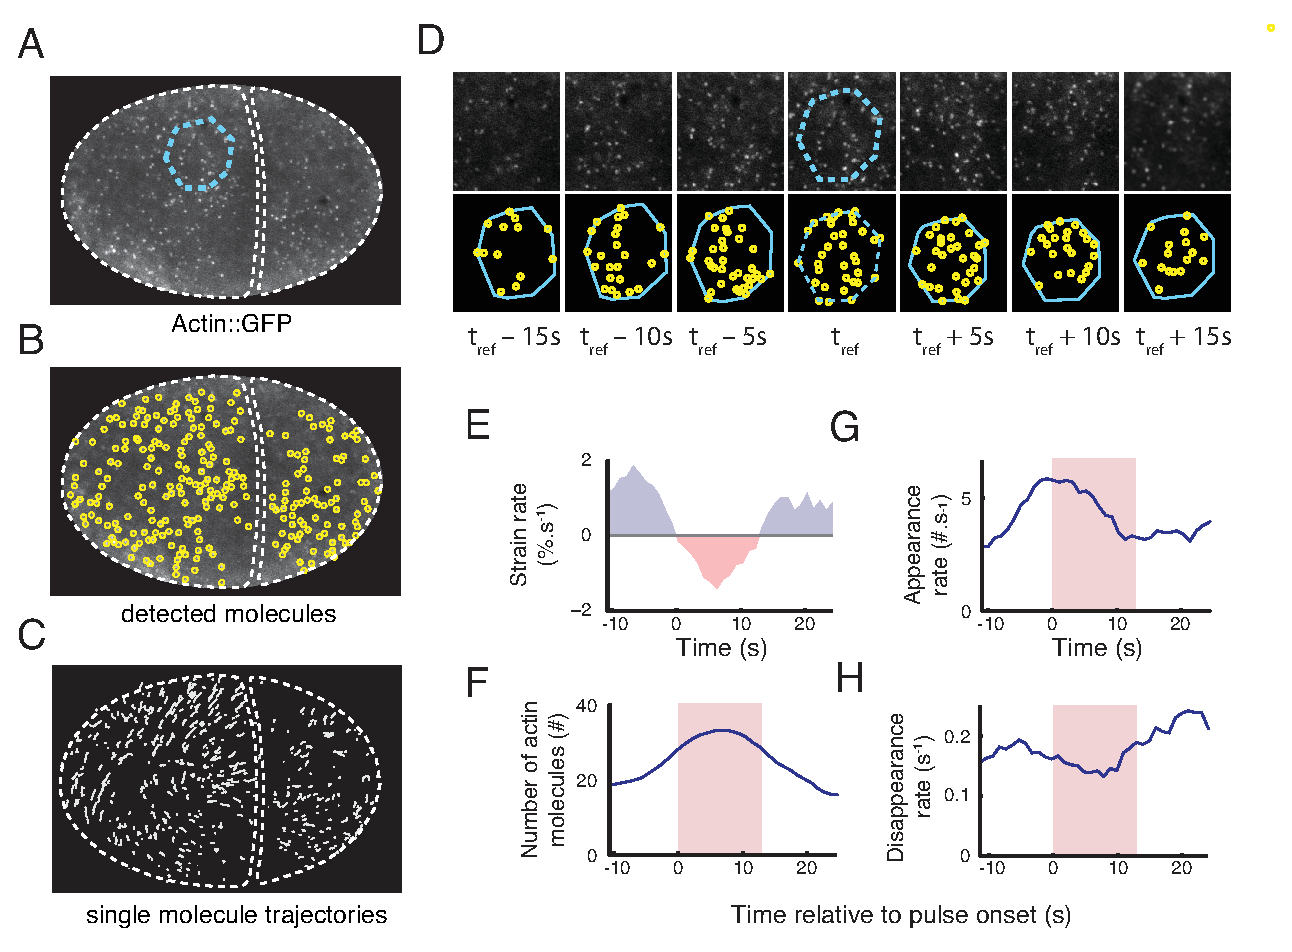
\includegraphics[width=1\textwidth]{Figure2-2}
\captionof{figure}[Single-molecule analysis of actin network assembly, disassembly and deformation during individual pulsed contractions.]{\textbf{Single-molecule analysis of actin network assembly, disassembly and deformation during individual pulsed contractions.} One frame of a time lapse sequence taken from an embryo expressing low levels of Actin::GFP. A patch of cortex undergoing a pulse is identified from the time lapse sequence, and outlined in cyan. (B) Automatic particle detection of single-molecules from the image in (A). (C) Trajectories of the molecules displayed in (B) that were tracked for longer than 2s. (D) A polygonal region of interest identified at time \(t = t_{ref}\), in (A) (dashed cyan polygon) is propagated forward and backward in time using the trajectories of tracked particles (see Materials and Methods). (E-H) Simultaneous measurements of single molecule dynamics and patch deformation over time. (E) Strain rate, measured using the particle-based method (see Materials and Methods). (F) Number of actin molecules in the patch. (G-H) Appearance rates (G) and disappearance rates (H) of actin molecules. Red shading in (F-H) indicates the time period in which the cortex is contracting locally (strain rate \(<\) 0).}
\end{figure}


If pulses are initiated by positive feedback in which local contraction concentrates actomyosin and/or its upstream regulators, then the onset of actomyosin accumulation should coincide with the onset of contraction. Contradicting this expectation, we found that, on average, Actin:GFP began to accumulate $\sim$5s before the onset of contraction (Figure 2.3B,F; Figure 2.11A-C), during a period of time in which the cortex was locally expanding (Figure 2.3A). Approximately 30$\%$ of the total increase in Actin::GFP single molecule density measured during a pulse occurred before the onset of contraction (Figure 2.11A-C). This initial accumulation was due entirely to a net imbalance of assembly and disassembly (Figure 2.3E): Before the onset of contraction, assembly rates increased (Figure 2.3C) and disassembly rates decreased (Figure 2.3D), leading to a sharp increase in the net rate of single molecule accumulation that peaked at the onset of contraction (Figure 2.3E).  During the contraction phase itself, the rate of change in single-molecule densities was determined almost entirely by a net imbalance of assembly/disassembly, with a very minor (\(<\) 6$\%$) contribution from contraction itself (Figure 2.3E). Assembly rates decreased steadily, and disassembly rates increased steadily, such that a transition from net assembly to net disassembly  (and from increasing density to decreasing density) occurred $\sim$7s sec after the onset of contraction (Figure 2.3E).  We obtained very similar results in embryos depleted of ARX-2, an essential subunit of the ARP2/3 complex (Figure 2.12), suggesting that our results are not biased by selective incorporation of Actin::GFP into branched vs unbranched F-actin \cite{Chen:2012dx}.

Single-molecule analysis of GFP-tagged Myosin II (NMY-2::GFP) revealed local assembly/disassembly dynamics that were strikingly similar to those measured for GFP::Actin. (Figure 2.3G-J). On average, the density of single molecules of NMY-2::GFP began to increase $\sim$6s before the onset of contraction during a period of local cortical expansion (Figure 2.3H), and approximately 50$\%$ of this increase occurred before the onset of contraction. As observed for GFP::Actin, the upswing in Myosin II before the onset of a contraction was associated with both a sharp increase in appearance rates and a sharp decrease in disappearance rates (Figure 2.3I,J); the net rate of increase peaked at the onset of contraction, and during the contraction phase, the appearance and disappearance rates returned steadily towards baseline levels.
In summary, we find that changes in actomyosin density during pulsed contractions are governed primarily by dynamic local imbalance of F-actin and Myosin II appearance and disappearance rates. A large fraction of the increase in F-actin and Myosin II density during each pulse occurs before the onset of contraction, and local contraction accounts for only a minor fraction of the subsequent density increase during the contraction phase itself. We conclude that changes in actomyosin density during pulsed contractions are governed primarily by dynamic modulation of assembly and disassembly, not by local clustering of these factors or by dynamical coupling of contraction and advection.


%Figure 2.2.3
\begin{figure}[!htbp]
\centering
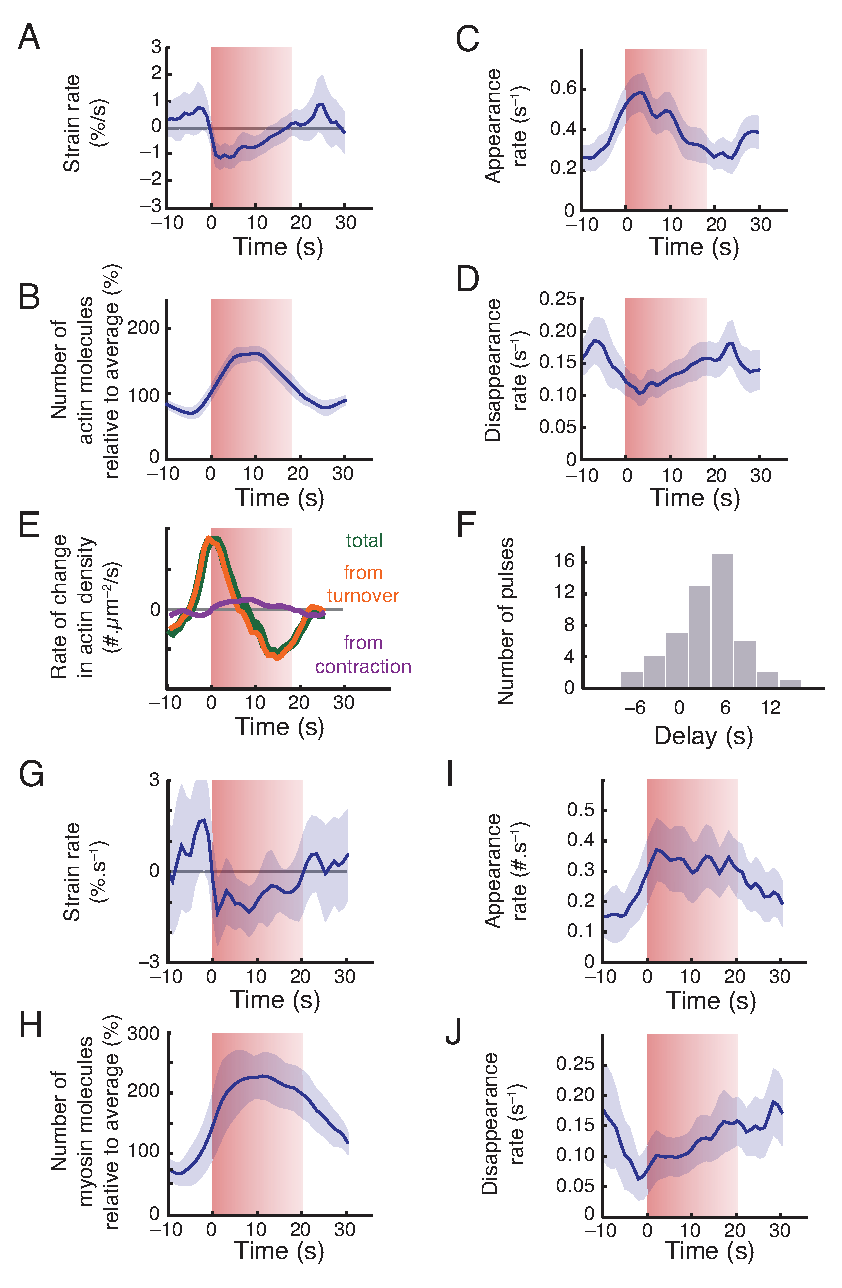
\includegraphics[width=0.7\textwidth]{Figure2-3}
\captionof{figure}[Spatiotemporal modulation of assembly and disassembly drives transient accumulation of F-actin and Myosin II during pulsed contractions.]{\textbf{Spatiotemporal modulation of assembly and disassembly drives transient accumulation of F-actin and Myosin II during pulsed contractions.} (A-D) Data from individual pulses, aligned with respect to the onset of contraction and then averaged to display particle-based strain rate (A), numbers of actin molecules (scaled by the average number for each pulse) (B) appearance rate (C), and disappearance rate (D) versus time.  (E) Total rate of change in actin density (green) and the individual contributions to rate of change from turnover and surface contraction. (F) Distribution of time delays between the initiation of contraction and actin accumulation. Data in (A-F) were averaged over 42 pulses, collected in 8 embryos. (G-J) Average myosin dynamics synchronized with respect to time at which myosin density reached peak levels during a pulse, displaying particle-based strain rate (G), number of molecules (scaled to the average number for each pulse) (H), appearance rate (I) and disappearance rate (J) versus time. Data were averaged over 30 pulses, collected in 5 embryos. Error bars: 95$\%$ confidence interval. }
\end{figure}



\subsection{Pulsed activation of RhoA drives the pulsed accumulation of F-actin and Myosin II}
The observation that F-actin and Myosin II accumulate with very similar kinetics during pulsed contractions suggests that their accumulation is driven by a common upstream regulator. An obvious candidate is the small GTPase RhoA (encoded by \textit{rho-1} in \textit{C.elegans}), which recruits and/or activates downstream effectors including formins, Rho Kinase (ROCK) and Anillin to control F-actin assembly and Myosin II activation in a variety of cell types \cite{Jaffe:2005kq, Piekny:2008jf}. RhoA activity is required for pulsed contractions in P0 \cite{Motegi:2006hi, Schonegg:2007if, Tse:2012fp}, and a biosensor for active RhoA derived from the RhoA binding domain of Anillin (henceforth GFP::AHPH) localizes to contractile foci in the zygote \cite{Tse:2011gd}. 

To determine if pulsed activation of RhoA accompanies pulsed contractions, we used a strain co-expressing GFP::AHPH \cite{Tse:2012fp} with an RFP-tagged version of the myosin heavy chain (NMY-2::RFP) to co-monitor RhoA activity and Myosin II accumulation during individual pulses in AB.  We observed a striking correlation between pulsed accumulation of GFP::AHPH and NMY-2::RFP during individual pulsed contractions (Figure 2.4A-C).  GFP::AHPH accumulated rapidly within a broad domain that prefigured the initial accumulation of NMY-2::RFP, reached a peak near the onset of visible contraction, and then began to disappear before NMY-2::RFP (Figure 2.4B,C). The initial accumulation of GFP::AHPH was diffuse, whereas NMY-2::RFP accumulated as discrete particles that increased in number and size before contracting together into a smaller and tighter central domain. During the falling phase of each pulse, the diffuse pool of GFP::AHPH at the outer edges of the initial domain disappeared rapidly, while a smaller and more persistent fraction of GFP::AHPH co-localized with NMY-2::RFP particles in the central domain (yellow arrows in Figure 2.4B; Figure 2.13).

%Figure 2.2.4
\begin{figure}[!htbp]
\centering
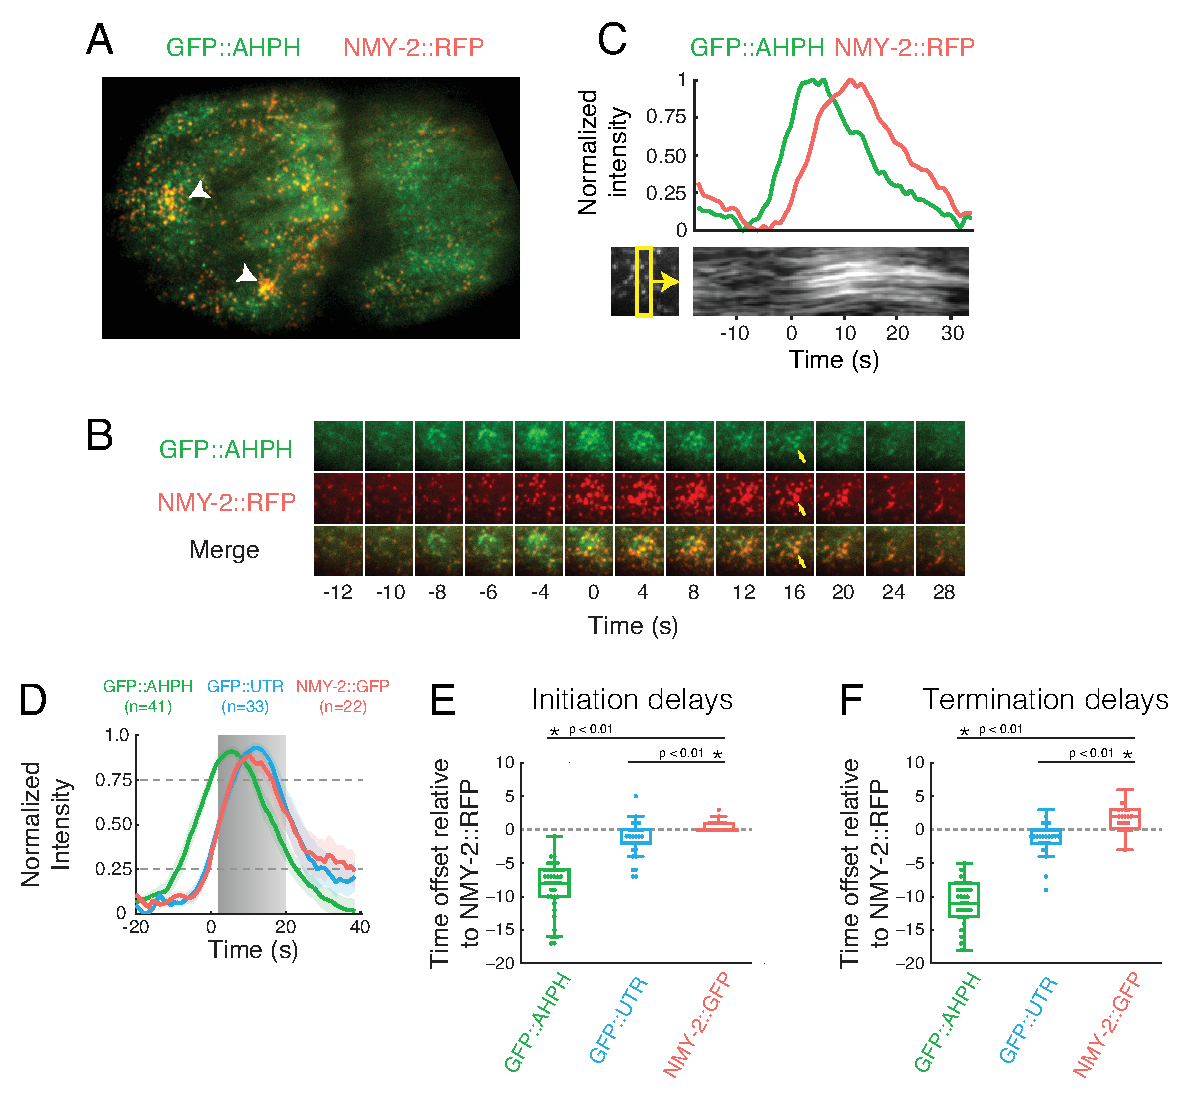
\includegraphics[width=0.9\textwidth]{Figure2-4}
\captionof{figure}[Local pulses of RhoA activation underlie pulsed accumulation and disappearance of F-actin and Myosin II.
]{\textbf{Local pulses of RhoA activation underlie pulsed accumulation and disappearance of F-actin and Myosin II.} (A) Micrograph of a 2-cell stage embryo expressing GFP::AHPH as a reporter for RhoA activity, and NMY-2::RFP. (B) Temporal dynamics of GFP::AHPH and NMY-2::RFP accumulation during a single pulse. The square region measures $\sim$5.3$\mu$m by 5.3$\mu$m. The time between frames is 2s for the first five frames, and 4s thereafter. (C) Above: Normalized fluorescence intensities of GFP::AHPH, and NMY-2::RFP. Below: A kymograph showing that local contraction (concerted movements of myosin puncta) begins after the accumulation of GFP::AHPH. The yellow box below left indicates the region used to generate the kymograph. (D) Comparison of averaged normalized fluorescence intensities vs time for active RhoA (GFP::AHPH), Myosin (NMY-2::GFP) and F-actin (GFP::UTR) from two-color data, co-aligned with respect to a common reference signal (NMY-2:RFP). Data were co-aligned with respect to the time at which NMY-2::RFP reaches 25$\%$ threshold. Hued regions report 95$\%$ confidence intervals. (E) Distribution of the delays between the onset of accumulation of NMY-2:RFP, and the onset of accumulation of GFP::AHPH, NMY-2::GFP and GFP::UTR. Onset of accumulation was measured as the time at which normalized probe intensity rose above 25$\%$ of its maximal level. (F) Distribution of the delays between the onset of disappearance of NMY-2:RFP, and the onset of disappearance of GFP::AHPH, NMY-2::GFP and GFP::UTR. Onset of disappearance was measured as the time at which normalized probe intensity fell below 75$\%$ of its maximal level. In boxplots, the central mark represents the median, the box indicates the 25th and 75th percentile, and the whiskers mark the minimum and maximum values}\end{figure}


To quantify these observations, we aligned data for multiple pulses from embryos co-expressing NMY-2::RFP and GFP::AHPH (see Materials and Methods). For each pulse, we smoothed and thresholded the NMY-2::RFP signal to identify a region of interest (ROI) containing high levels of NMY-2::RFP just before the onset of contraction (Figure 2.12A; Materials and Methods). We propagated this ROI forward and backwards in time (see Figure 2.12A, Materials and Methods), and then measured the mean intensities of the RFP and GFP signals within the ROI before, during and after the pulse (Figure 2.12B,C). We normalized these data with respect to the minimum (pre-contraction) and maximum intensities measured during this interval, then aligned data for multiple pulses with respect to the time point at which NMY-2::RFP reached 25$\%$ of its maximum intensity (Figure 2.4D, Materials and Methods). These aligned data confirm that sharp increases and decreases in RhoA activity precede, respectively, the appearance and disappearance of NMY-2::RFP (Figure 2.4D).  On average, GFP::AHPH reaches 25$\%$ of its maximum intensity 8.6 +/- 3.9 seconds before NMY-2::RFP (Figure 2.4E), and falls below 75$\%$ of its maximum intensity 11.1 +/- 3.5 seconds before NMY-2::RFP (Figure 2.4F).

We used the same approach to align data for embryos co-expressing NMY-2::RFP and either the F-actin binding domain of Utrophin fused to GFP (GFP::UTR); a marker for F-actin \cite{Burkel:2007fj,Tse:2012fp}, or GFP::Anillin \cite{Maddox:2007cx}. Using NMY-2::RFP as the common reference to co-align data for NMY-2::RFP, GFP::AHPH, GFP::UTR and GFP::Anillin, we found that like Myosin II, F-actin and Anillin accumulate and dissipate during pulsed contractions with a significant delay relative to GFP::AHPH (Figure 2.4D-F, Figure 2.13A-D). Thus local activation and inactivation of RhoA precedes and times the accumulation and disappearance of its downstream targets. 

Finally, we used the time points at which NMY-2::RFP intensities (Figure 2.4D) and single molecule densities of Myosin::GFP (Figure 2.3H) reached 25$\%$ of their peak values to align the time course of RhoA activation with respect to the onset of contraction as measured by single molecule imaging.  This analysis shows that RhoA activity peaks just before the onset of contraction (indicated by gray box in Figure 2.4D) and thus local concentration of active RhoA by advection-contraction \cite{Munjal:2015bx} cannot explain the rising phase of RhoA activation in \textit{C.elegans} embryos.  By extension, the same analysis reveals that RhoA activity peaks and begins to fall at a point where F-actin and Myosin II disappearance rates are at a minimum (Figure 2.3D,J); thus factors other than cortical actomyosin disassembly drive the disappearance of active RhoA at the end of a pulse.

Using the same two-color image analysis, we confirmed that pulses of RhoA activity accompany pulsed contractions in the zygote P0. To remove the potentially confounding effects of large scale cortical flows that occur during zygotic polarization, we performed these measurements in embryos depleted of the centrosomal factor SPD-5 \cite{Munro:2004jk, Hamill:2002tw}, which exhibit pulsed contractions but lack cortical flows. In \textit{spd-5}(RNAi) P0 zygotes, as in wild-type AB cells, increases and decreases in local GFP::AHPH intensity preceded the rise and fall of NMY-2::RFP (Figure 2.14A-F) and to a lesser extent GFP::UTR (Figure 2.14D-F) and GFP::Anillin (Figure 2.13E-H).  As in AB, the initial accumulation of GFP::AHPH was broad and diffuse while a more persistent pool of GFP::AHPH remained concentrated within punctae that co-localized with NMY-2::RFP within a more central region of the initial domain (yellow arrows in Figure 2.14B). 

\subsection{Pulsed activation of RhoA does not require Myosin II.}
Recent studies suggested that active RhoA and Myosin II accumulate with similar timing during pulsed apical contractions in the \textit{Drosophila} germband, and that Myosin II activity is required for pulsed accumulation of active RhoA \cite{Munjal:2015bx}. Our observation that active RhoA peaks before the onset of contraction rules out models in which local contraction concentrates RhoA, or its upstream activators, to initiate pulses. However, it remains possible that Myosin II activity is otherwise required for pulsed activation of RhoA. To test this possibility, we used RNAi to deplete the Myosin heavy chain NMY-2 in a strain co-expressing transgenic GFP::AHPH and NMY-2 tagged with mKate2 at the endogenous locus by CRISPR-mediated homologous recombination (NMY-2::mKate2, a kind gift of Dan Dickinson).  We used RNAi against NMY-2 to deplete NMY-2::mKate2 to the point where only a few single NMY-2::mKate particles could be detected at the P0 cortex using imaging conditions that allow robust detection of single molecules (Figure 2.5A). Under these conditions, in \textit{nmy-2} RNAi zygotes, we still observed transient focal accumulations of GFP::AHPH (Figure 2.5A,B).  These accumulations were roughly similar in size and spacing to those observed in \textit{spd-5} (RNAi) zygotes during polarity establishment, and many occurred on patches of cortex in which fewer than two discrete particles of NMY-2::mKate were detected, excluding any possible contribution from contractile tension generated by Myosin II (Figure 2.5B). Aligning GFP::AHPH intensities vs time across many pulses in \textit{nmy-2}(RNAi) zygotes revealed a mean time course for AHPH accumulation and dissipation that is comparable to that measured for the diffuse pool of GFP::AHPH in \textit{spd-5} (RNAi) zygotes (Figure 2.5C).  Indeed, pulses terminated more rapidly in \textit{nmy-2}(RNAi) than in \textit{spd-5} (RNAi) zygotes, implying that neither Myosin II activity nor its inhibition is required for rapid pulse termination. We conclude that Myosin II is not required for locally pulsatile activation of RhoA in \textit{C.elegans} embryos, although myosin activity may shape spatiotemporal pulse dynamics (see Discussion).

%Figure 2.2.5
\begin{figure}[!htbp]
\centering
\includegraphics[width=1\textwidth]{Figure2-5}
\captionof{figure}[Myosin II is not required for the pulsed activation of RhoA.]{\textbf{Myosin II is not required for the pulsed activation of RhoA.} (A) Comparison of pulse dynamics in zygotes expressing GFP::AHPH and NMY-2::mKATE and treated with either \textit{spd-5}(RNAi) or \textit{nmy-2}(RNAi). Top panels show myosin localization (NMY-2::mKATE), middle panels show RhoA activity (GFP::AHPH). Bottom panels are kymographs showing GFP::AHPH dynamics over time.  Dashed yellow rectangles in middle panel indicate the regions from which the kymographs were made. Vertical yellow arrows indicate a region undergoing repeated pulses. Intensities were scaled identically for \textit{spd-5}(RNAi) and \textit{nmy-2}(RNAi) zygotes. (B) Top: Mean intensities of NMY-2::mKATE (red) and GFP::AHPH (green) vs time for a single pulse in an \textit{nmy-2}(RNAi) zygote. Bottom: sequential snapshots of the region undergoing the pulse showing NMY-2::mKATE (red) and GFP::AHPH (green) distributions. Yellow arrowheads indicate the  1-2 particles that can be detected in the region undergoing a pulse. (C) Mean intensity of GFP::AHPH over time in \textit{nmy-2}(RNAi) and \textit{spd-5}(RNAi) zygotes, aligned with respect to the time at which the normalized signal reaches 25$\%$ of its maximum value.  For \textit{spd-5} (RNAi) zygotes, the signal was measured either within the entire boxed region in which each pulse occurred  or at its periphery (see Figure 2.2.12 for details). Hued regions report 95$\%$ confidence intervals.}
\end{figure}



\subsection{RhoA feeds back locally to promote its own activity and this is required for pulse initiation.}
A recent study described propagating cortical waves of RhoA activity in echinoderm oocytes and frog embryos; these appear to be driven by locally excitable RhoA dynamics in which RhoA feeds back positively to promote its own activation and negatively, through local F-actin assembly, to promote delayed inactivation \cite{Bement:2015jp}.  We hypothesized that a similar combination of positive and negative feedbacks could drive local pulses of RhoA activity in \textit{C.elegans} embryos.  Plotting the rate of change in GFP::AHPH intensity vs intensity during the rising phase of individual pulses in either P0 or AB cells revealed a sharp increase in the rate of RhoA activation with increasing RhoA (Figure 2.6A). This is consistent with a scenario in which active RhoA feeds back positively to promote further activation of RhoA.  However, it could also reflect pulsed activation of RhoA (without feedback) by an upstream activator.  To distinguish these possibilities, we used RNAi to progressively deplete embryos of RhoA. If the time course of RhoA activation is dictated by an upstream activator, we should observe pulsed accumulation of GFP::AHPH as long as it remains detectable at the cortex. In contrast, if positive feedback of RhoA onto itself drives pulse initiation, then there should be an abrupt loss of pulsing below a threshold level of RhoA.  Consistent with the latter expectation, we observed an abrupt transition from pulsed to non-pulsed RhoA accumulation after $\sim$ 12 hours of feeding (Figure 2.6B,C).  In zygotes that lacked pulsed RhoA accumulation, we could still readily detect robust RhoA-dependent cortical flows \cite{Motegi:2006hi, Schonegg:2006ed} during polarity establishment (dashed yellow lines in Figure 2.6B) and localized accumulation of active RhoA prior to cytokinesis (cyan arrowheads in Figure 2.6B).  Together, these observations support the idea that RhoA feeds back positively to amplify its own activation and that sufficiently strong feedback is required to generate local pulses of high RhoA activity. 


%Figure 2.2.6
\begin{figure}[!htbp]
\centering
\includegraphics[width=1\textwidth]{Figure2-6}
\captionof{figure}[RhoA activation is autocatalytic.]{\textbf{RhoA activation is autocatalytic.} (A) The time derivative of normalized RhoA activity (GFP::AHPH) plotted vs normalized activity during the early phase of pulse initiation in P0 (top panel, n = 40 pulses) and AB (bottom panel, n = 41 pulses). Error bars: 95$\%$ confidence interval. (B-C) Analysis of pulse dynamics in embryos progressively depleted of RHO-1 by RNAi.  (B) Top panels show GFP::AHPH distributions in interphase embryos from mothers subjected to no (wild type), 10 hours and 13 hours of \textit{rho-1}(RNAi). Middle panels  show kymographs from the same embryos illustrating spatiotemporal dynamics of GFP::AHPH  from interphase through cytokinesis.  Dashed yellow lines indicate approximate pattern of cortical flow.  Cyan arrowheads indicate accumulation of GFP::AHPH just prior to cytokinesis.  (C) Timeline indicating the presence (magenta circles) or absence (cyan circles) of pulsing in embryos treated with \textit{rho-1}(RNAi) for the indicated times, revealing an abrupt transition from pulsing to no pulsing at $\sim$12 hours post-treatment.}
\end{figure}

\subsection{Delayed accumulation of the Rho GAPs RGA-3/4 underlies pulse termination.}
What terminates RhoA activity during each pulse? Our results imply that local termination of RhoA activity at the end of a pulses does not require Myosin II activity or (by extension) its local inhibition by Myosin phosphatase \cite{Piekny:2002vx, Piekny:2003iv, Diogon:2007kc}, nor is it timed by cortical disassembly. Previous studies identified the redundant RhoA GAPs RGA-3 and RGA-4 as inhibitors of RhoA activity during polarization and cytokinesis \cite{Schonegg:2007if, Zanin:2013el, Schmutz:2007jq, Tse:2012fp}. A YFP-tagged RGA-3 transgene accumulates at the cortex in early embryos \cite{Schonegg:2007if}, and simultaneous depletion of RGA-3 and RGA-4 leads to hyper activation of RhoA and hypercontractility during zygotic polarization \cite{Schonegg:2007if, Schmutz:2007jq, Tse:2012fp}.  We wondered, therefore, if RGA-3/4 could provide negative feedback to terminate RhoA activity during individual pulses.
To test this possibility, we first imaged embryos co-expressing GFP::RGA-3 and NMY-2::mKATE. Focusing on AB, and using 2-color analysis as above, we confirmed that GFP::RGA-3 is present throughout the cortex, but accumulates locally during individual pulsed contractions (Figure 2.7A-C). Significantly, GFP::RGA-3 and NMY-2::mKATE accumulated with very similar timing (Figure 2.7B). Using NMY-2::mKATE and NMY-2::RFP  as common signals to co-align data for GFP::AHPH and GFP::RGA-3, we inferred that, on average, GFP::RGA-3 accumulates with a $\sim$6 sec delay relative to GFP::AHPH. The rate of RhoA activation peaks before the onset of GFP:RGA-3 accumulation, and rapid accumulation of GFP::RGA-3 coincides with deceleration and then reversal of RhoA activation (Figure 2.7C, bottom). Together, these observations suggest that delayed accumulation of RGA-3/4 plays a key role in terminating each pulse of RhoA activity. To test this further, we created a strain in which GFP::AHPH and NMY-2::mKATE were co-expressed in \textit{rga-3;rga-4} (hereafter \textit{rga-3/4}) double mutant embryos \cite{Zanin:2013el}. Consistent with previous reports \cite{Schonegg:2007if, Zanin:2013el, Schmutz:2007jq, Tse:2012fp}, during polarity establishment in P0 in \textit{rga-3/4} double mutant embryos, we observed hyper-accumulation of GFP::AHPH and hypercontractility that was characterized by a sequence of convulsive contractions of the anterior cortex and rapid anterior directed cortical flows (Figure 2.7D, 2nd column).  However, we could no longer detect local pulses of GFP::AHPH in these embryos.  In principle, this could be because rapid flows sequester factors required for pulsed contractility to the extreme anterior pole. To exclude this possibility, we used partial depletion of the myosin regulatory light chain (MLC-4) to attenuate contractility and cortical flows in \textit{rga-3/4} double mutant zygotes or in control zygotes that were doubly heterozygous for \textit{rga-3} and \textit{rga-4} (Figure 2.7D).  In control zygotes partially depleted of MLC-4, cortical flows were sharply reduced, but pulsed accumulation of GFP::AHPH could be readily detected (Figure 2.7D, 3rd column). By contrast, in \textit{rga-3/4} double mutant zygotes partially depleted of MLC-4, cortical flows during polarity establishment phase were slower than observed in wild type embryos; GFP::AHPH was uniformly enriched, but we did not observe local pulses of GFP::AHPH accumulation (Figure 2.7D, 4th column).  Together, these data suggest that negative feedback through delayed accumulation of RGA-3/4 plays a key role in terminating local pulses of RhoA activity.


%Figure 2.2.7
\begin{figure}[!htbp]
\centering
\includegraphics[width=0.85\textwidth]{Figure2-7}
\captionof{figure}[Delayed accumulation of RGA-3/4 mediates negative feedback required for pulse termination.]{\textbf{Delayed accumulation of RGA-3/4 mediates negative feedback required for pulse termination.} (A) Micrograph of a 2-cell stage embryo expressing GFP::RGA-3 (green) and NMY-2::RFP (red). (B) Temporal dynamics of a single pulse. The square region measures 6.4$\mu$m by 6.4$\mu$m. (C) Top: Averaged normalized fluorescence intensities vs time for NMY-2::RFP and GFP::RGA-3 from two-color data, co-aligned with respect to the time at which NMY-2::RFP reaches 25$\%$ threshold. The averaged normalized fluorescence intensity of GFP::AHPH, co-aligned with NMY-2::RFP.  Bottom: The averaged time derivative of the normalized GFP::AHPH intensity, again co-aligned using NMY-2::RFP.  Hued regions report 95$\%$ confidence intervals. (D) (top panels) Distributions of GFP::AHPH during interphase in zygotes  with the indicated genotypes.  (bottom panels) Kymographs showing patterns of GFP::AHPH distribution and redistribution during interphase for the same genotypes. Micrographs of 1-cell stage embryos expressing GFP::AHPH. RhoA exhibits pulsatile activity in \textit{rga-3/4}(+/-) embryos (control n=4 embryos, \textit{mlc-4} RNAi n=6 embryos) but not \textit{rga-3/4}(-/-) embryos (control n=9 embryos, \textit{mlc-4} RNAi n=8 embryos).}
\end{figure}

Recent work suggests that F-actin accumulation mediates delayed inhibition of RhoA activity in echinoderm and frog oocytes and embryos \cite{Bement:2015jp}.  We wondered if F-actin might play a similar role in \textit{C.elegans} embryos by mediating recruitment of RGA-3/4.  Consistent with this possibility, two-color imaging of GFP::RGA-3 and mCherry::Lifeact  (a marker for F-actin  \cite{Pohl:2012bg}) revealed extensive co-localization of RGA-3 and F-actin in both P0 and AB (Figure 2.8A).  A substantial fraction of GFP::RGA-3 co-localized with mCherry::Lifeact in extended linear structures that presumably represent actin filaments and/or small filament bundles. Treating permeabilized zygotes \cite{Carvalho:2011ce, Olson:2012cs} with Latrunculin A to depolymerize F-actin lead to a profound loss of cortical GFP::RGA-3, supporting the idea that F-actin plays a key role in recruiting RGA-3/4 to the cortex during individual pulses (Figure 2.8B).




%Figure 2.2.8
\begin{figure}[!htbp]
\centering
\includegraphics[width=1\textwidth]{Figure2-8}
\captionof{figure}[Cortical RGA-3/4 localization depends on F-actin]{\textbf{Cortical RGA-3/4 localization depends on F-actin} (A) Micrographs of P0 (top) and AB (bottom) embryos co-expressing GFP::RGA-3 and mCherry::LifeAct. (B) Zygote co-expressing GFP::RGA-3 and mCherry::LifeAct before (top) and $\sim$90s after (bottom) treatment with 10µM Latrunculin A.}
\end{figure}



\subsection{Fast positive and delayed negative feedback involving RhoA and RGA-3/4 can account quantitatively for locally pulsatile RhoA dynamics.}
Our data suggest that locally excitable RhoA dynamics could arise independently of myosin activity through a combination of fast positive feedback on RhoA activity and delayed negative feedback via local recruitment of RGA-3/4 (Figure 2.9A).  To ask if this combination of feedback loops is sufficient to generate locally pulsatile activity, we formulated a simple ordinary differential equation model, describing local rates of change in RhoA and RGA-3/4, based on the following assumptions:  (a)  RhoA is activated at a basal rate, and feeds back positively to promote further RhoA activation, (b) RhoA feeds forward through F-actin assembly to promote local, reversible, association of RGA-3/4 with the cortex and (c) RGA-3/4 acts as a GAP to promote local inactivation of RhoA. Consistent with our experimental observations (Figure 2.6A) , we assumed that autoactivation of RhoA is a saturating function of RhoA activity, represented by a Hill function with Hill coefficient n = 1. We assumed that inactivation of RhoA by RGA-3/4 obeys Michaelis-Menten kinetics. To account for the observed delay between an increase in RhoA and the sharp onset of RGA-3/4 accumulation (Figure 2.7C), we assumed ultrasensitive dependence of RGA-3/4 accumulation rate on RhoA, with the steepness of the response governed by an exponent m (see Materials and Methods for mathematical details). 



%Figure 2.2.9
\begin{figure}[!htbp]
\centering
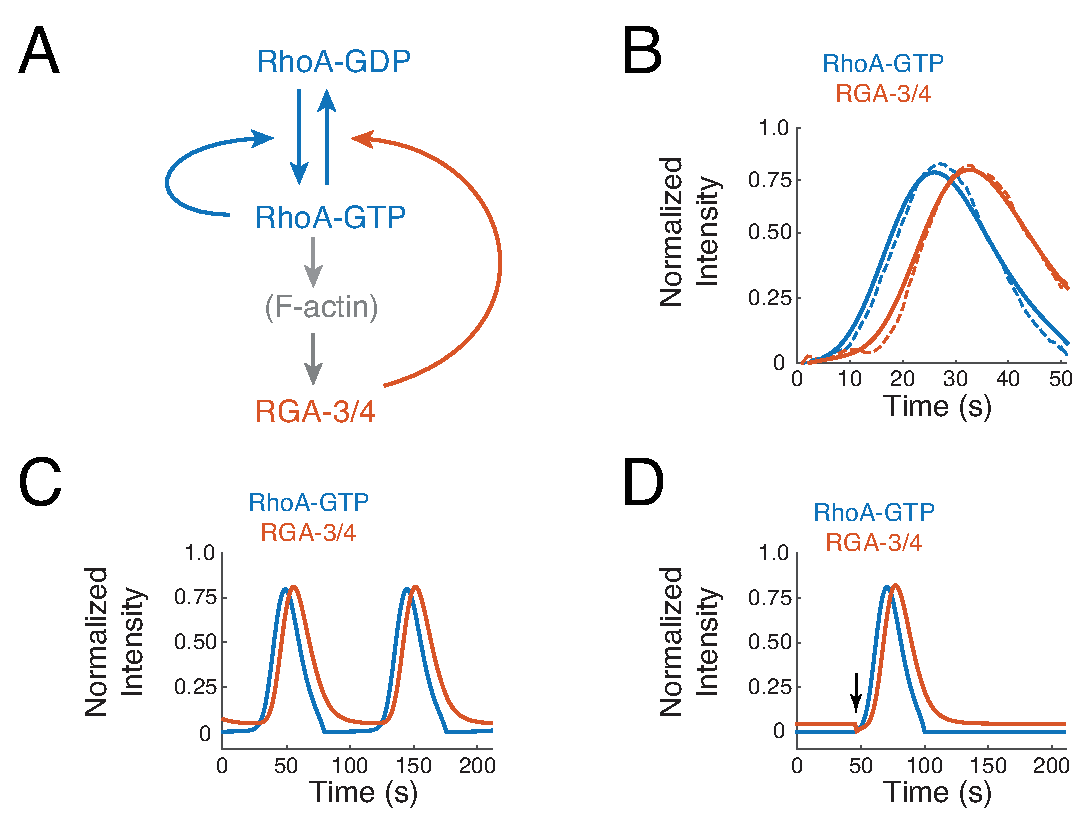
\includegraphics[width=1\textwidth]{Figure2-9}
\captionof{figure}[Autocatalytic RhoA activation and delayed negative feedback through RGA-3/4 is sufficient to produce locally excitable RhoA dynamics.]{\textbf{Autocatalytic RhoA activation and delayed negative feedback through RGA-3/4 is sufficient to produce locally excitable RhoA dynamics.} (A) Schematic representation of the simple mathematical model used to model RhoA pulse dynamics. (B) Comparison between measured (dashed lines) and simulated (solid lines) pulse dynamics for the case in which n = 1, $k_{r}^0 = 0.005$, $k_{p}^0 = 0.006$.  The remaining model parameters were estimated by fitting data ($m=1.5289$, $K_{fb}=0.4581$, $K_{GAP}=0.001$, $k_{r}^{ass}=0.1592$, $k_{r}^{diss}=0.1101$; see Materials and Methods for details).  (C) Simulation dynamics for the parameter values in (B) are oscillatory, with pulses occurring at regular intervals.  (D)  A small change in the basal RhoA activation rate from $k_{p}^0 = 0.006$ to $k_{p}^0 = 0.004$ results in excitable dynamics in which a stable rest state can be destabilized by a transient reduction of RGA-3/4 (vertical black arrow) to trigger a single pulse of RhoA activity.}
\end{figure}



We set values for basal RhoA activation and RGA-3/4 recruitment rates based on the slow rates of increase in GFP::AHPH and GFP::RGA-3 observed before the sharp upswing of each pulse (Figure 2.7C). Then we estimated values for the model's remaining parameters by fitting the relationships between the local rates of RhoA activation and RGA-3/4 recruitment and the local densities of RhoA and RGA-3/4 inferred from averaged and co-aligned GFP::AHPH and GFP::RGA-3 intensities  (Figure 2.7C; see Materials and Methods for details).   For these choices of parameters,  without any further adjustments, the model predicts oscillatory dynamics, with a pulse waveform that matches closely that measured for pulses in AB cells (Figure 2.9B,C).  

Interestingly, the dynamics could be tuned by small decreases in the basal RhoA activation rate (Figure 2.9D) or small increases in the basal RGA-3/4 recruitment rate (not shown), into a regime in which the dynamics are excitable - i.e., there is a stable state and a transient local input is required to trigger a pulse of RhoA activity (Figure 2.9D).  This is consistent with our observations in \textit{nmy-2}(RNAi) embryos that some patches of cortex are quiescent while others exhibit repeated pulses of activity at regular intervals (yellow arrows in Figure 2.5A). We conclude that a simple combination of positive and negative feedback loops, coupling local RhoA activity and RGA-3/4 accumulation, is in principle sufficient to explain pulsatile RhoA dynamics in early \textit{C.elegans} embryos, independent of actomyosin contractility.





\section{Discussion}
Pulsed contractility is a widespread mode of actomyosin contractility, but its mechanistic basis has remained poorly understood \cite{Levayer:2012bu, Gorfinkiel:2016bv}. Current models for pulsed contractility invoke mechanochemical feedback in which contractile forces produced by Myosin II couple in different ways with actomyosin assembly/disassembly to drive excitable or oscillatory dynamics. Proposed feedback mechanisms include tension-dependent motor binding kinetics \cite{Ren:2009ep, Effler:2006hc, He:2010gf, Luo:2012bl}, tension-dependent filament assembly/stabilization \cite{Hayakawa:2011dq, DeLaCruz:2015dj} or disassembly \cite{Machado:2014fx}, tension-dependent activation of Myosin II via Ca++ \cite{Kapustina:2008ds} or RhoA \cite{Koride:2014hp}, or modes of feedback in which local contraction advects and concentrates actomyosin and/or its upstream activators \cite{Bois:2011kx, Kumar:2014ux, Munjal:2015bx}.  Here, we have identified a mechanism for pulse generation that does not require force production or redistribution of cortical factors by Myosin II.  Using single molecule imaging and particle tracking analysis, we have shown that the rapid initial accumulation of F-actin and Myosin II begins well before the onset of contraction, at a time when the cortex is locally expanding; Redistribution of actomyosin by local contraction makes a minor contribution to the overall accumulation of actomyosin during each pulse.  Instead, our data show that pulsed accumulation and disappearance of F-actin and Myosin II are determined primarily by local modulation of their assembly/recruitment and disassembly. Using two-color imaging, we have shown that during each pulse, active RhoA begins to accumulate well before its downstream targets F-actin, Myosin II and Anillin. Active RhoA nearly reaches its peak level before the onset of contraction (Figure 2.4D), and then it begins to disappear well before its downstream targets. Significantly, locally pulsed activation of RhoA continues to occur on patches of cortex that contain only a few (1-2) particles of Myosin II, which presumably are insufficient to produce local contractile stress. Thus a Myosin-independent RhoA pulse-generator underlies pulsed contractility in early \textit{C.elegans} embryos.

The pulses of RhoA activity described here and in other contexts \cite{Munjal:2015bx, Bement:2015jp, Mason:2016bs} are strikingly reminiscent of excitable behaviors found in other systems, such as action potentials in neuronal \cite{Izhikevich:2007aa} or cardiac cells \cite{Luo:1991vz}, or transient pulses of intracellular calcium release \cite{Goldbeter:1996aa}, or pulses of actin assembly observed in motile cells \cite{Weiner:2007cl}. Theoretical studies highlight two key ingredients for excitable dynamics: fast positive feedback and delayed negative feedback \cite{Strogatz:1994tz}. The sharp acceleration of active RhoA accumulation that we observe during the early rising phase of individual pulses is a dynamical signature of fast positive feedback in which RhoA promotes its own activity. Stronger evidence that RhoA participates in a positive feedback loop that is essential for pulsing comes from our observation that depletion of RhoA below a certain threshold leads to an abrupt loss of pulsed contractions, while having minimal effects on other RhoA-dependent functions such as cortical flow during polarization\cite{Motegi:2006hi, Schonegg:2006ed} or cytokinesis \cite{Loria:2012ks}. 

The mechanism for this feedback remains unclear.  Because the initial acceleration of RhoA activation occurs before any visible accumulation of Myosin II, Anillin or F-actin, it is unlikely that accumulation of these downstream targets makes a significant contribution to positive feedback.  A more likely possibility is that RhoA feeds back through one or more of its upstream activators, such as ECT-2, CYK-4 and NOP-1 \cite{Tse:2012fp}.  For example, during cytokinesis, active RhoA can act as a cofactor to promote transactivation of the RhoGEF ECT-2 by the RhoGAP CYK-4 \cite{Zhang:2015bx}.  While CYK-4 is not required for pulsed activation of RhoA during polarization \cite{Tse:2012fp}, it is possible that RhoA could feedback through NOP-1, a protein of unknown activity that is required for RhoA activation during interphase in P0 and AB \cite{Tse:2012fp}. Identifying the molecular mechanism(s) for this feedback is an important goal for future studies.


Our data suggest that the redundantly acting RhoGAPs RGA-3/4 play a key role in providing the delayed negative feedback that terminates RhoA pulses. RGA-3/4 act as GAPs towards RHO-1 in vitro \cite{Schonegg:2007if}, and loss of RGA-3/4 leads to hyperactivation of RhoA in vivo \cite{Tse:2012fp}.  We find that during each pulse, RGA-3 accumulates with a delay of $\sim$6 seconds relative to active RhoA. Significantly, \textit{\textbf{the rate}} of active RhoA accumulation peaks, and begins to fall, just as GFP::RGA-3 begins to accumulate, suggesting that rapid accumulation of RGA-3/4 plays a key role in timing the end of each RhoA pulse. Consistent with this possibility, pulsatile RhoA activation is completely abolished in \textit{rga-3/4} double mutant zygotes, even when contractility is attenuated to prevent sequestration of RhoA activators by hyperactive cortical flow.  A similar dependence of pulsatility on a RhoA GAP has recently been reported in the context of ventral furrow invagination in \textit{Drosophila} \cite{Mason:2016bs}.

Together, these data suggest a model for locally excitable RhoA dynamics in which RhoA feeds back positively to promote its own activation, and feeds back negatively with a delay through RGA-3/4 to promote its own inactivation. Indeed, when we formulate this model mathematically, and constrain model parameter values to match the local dependencies of RhoA and RGA-3/4 accumulation rates on levels of RhoA and RGA-3/4 inferred from two-color imaging data, the model predicts locally pulsatile RhoA dynamics, and small tunings of the model's parameters  mediate interconversion between excitable dynamics and spontaneous oscillations.  This simple modeling exercise establishes an internally consistent hypothesis for pulsatile contractility that can be confirmed and extended by future experiments.

What governs the recruitment of RGA-3/4 during each pulse?  We have found that GFP::RGA-3 co-localizes broadly and extensively with cortical F-actin in both P0 and AB. RGA-3/4 accumulates with the same timing as F-actin during each pulse, and depolymerizating F-actin abolishes this accumulation.  This suggests a specific mechanism for delayed recruitment of RGA-3/4 in which RhoA promotes increased local F-actin assembly (potentially through the formin CYK-1 \cite{Severson:2002ve}), and F-actin in turn recruits RGA-3/4.  Interestingly, a recent study\cite{Bement:2015jp} suggests that RhoA and cortical F-actin form an excitable circuit, with RhoA as activator and F-actin as inhibitor, that propagates cortical waves of RhoA activity and F-actin assembly in oocytes and embryonic cells of frogs and echinoderms.  The mechanism(s) by which F-actin feeds back to inactivate RhoA in these cells remains unknown, but our observations in \textit{C.elegans} support to the idea, proposed by Bement et al, 2015, that a  RhoGAP homologous (or analogous) to RGA-3/4 may be recruited by F-actin to mediate negative feedback in frog and echinoderm cells. A similar circuit design may underlie the propagation of actin waves observed in many motile cells (reviewed in \cite{Allard:2013if}).

It is also interesting to compare our observations to those made recently in the \textit{Drosophila} germband \cite{Munjal:2015bx}. In germband cells, pulsed accumulation of a RhoA biosensor appears to coincide with the local accumulation of F-actin and Myosin II, and with the onset of contraction, and it is abolished by inhibition of Rho Kinase, an upstream activator of Myosin II.  In \textit{C.elegans}, by contrast, pulsed accumulation of the analogous biosensor (based on a fragment of Anillin that binds active RhoA) precedes actomyosin accumulation and the onset of contraction by many seconds and persist in the almost complete absence of Myosin II.

To some extent, these differences could reflect the imaging methods used to detect the RhoA biosensor.  Using near-TIRF imaging in \textit{C.elegans} embryos, we detect two pools of the biosensor: a diffuse pool that begins to accumulate well before Myosin II, and a second more punctate pool whose distribution strongly overlaps with Myosin II (Figure 2.4B, Figure 2.12F&G, Figure 2.14.  Based on studies in other cells \cite{Weiner:2007cl}, the diffuse pool may be more difficult to detect using confocal microscopy. Thus it remains possible that a diffuse pool of active RhoA accumulates before actomyosin in the \textit{Drosophila} germband, but escapes detection by confocal microscopy.  

An alternative idea is that pulsed contractility is governed by locally excitable RhoA dynamics in both systems, but that different forms of positive feedback may contribute differently to driving the rapid upswing of RhoA activity, and that different mechanisms may operate to trigger pulses (by driving RhoA activity above a threshold for excitation). For example, in the \textit{Drosophila} germband, a mode of feedback in which local contraction advects and concentrates active RhoA (or upstream activators) may be required to initiate pulses, whereas in \textit{C.elegans}, local fluctuations in RhoA or RGA-3/4 levels may be sufficient to do so in the absence of contractility. Importantly, in the \textit{Drosophila} germband, as in \textit{C.elegans}, advection/contraction coupling accounts for only a fraction of the total accumulation of active RhoA during each pulse; thus other modes of positive feedback must also make a significant contribution. 
More generally, we hypothesize that the different modes of RhoA excitability that have been described in frog, echinoderm, \textit{C.elegans} and \textit{Drosophila} embryos share a deeper underlying mechanistic origin. We suggest that a comparative analysis of mechanisms for pulsing in these and other systems will be a very fruitful way to uncover core conserved circuitry for pulse generation and to understand the ways in which this core circuitry is tuned or accessorized in different contexts to achieve different functional outcomes.  




\section{Materials and Methods}
\subsection{C. Elegans culture and strains}
We cultured C. elegans strains at 22$^{\circ}$C under standard conditions \cite{Brenner:1974wn} Table 2.1 lists the mutations and transgenes used in this study. Unless otherwise specified, strains were provided by the Caenorhabditis Genetics Center, which is funded by the National Institutes of Health (NIH) National Center for Research Resources.



\subsection{RNA interference}
RNAi was performed by the feeding method as previously described \cite{Timmons:2001wg}.  Bacteria targeting \textit{nmy-2}, \textit{spd-5}, \textit{rho-1}, \textit{perm-1}, \textit{arx-2} and \textit{mlc-4} were obtained from the Kamath feeding library \cite{Kamath:2003bk}. The L4417 plasmid targeting the entire GFP sequence (generated by the Fire lab and available at http://www.addgene.org/1649/) was transformed into HT115(DE3) bacteria. For the Myosin depletion experiments, L4 larvae co-expressing GFP::AHPH and NMY-2::mKate2  were transferred to \textit{nmy-2} RNAi feeding plates 24-30 hours before imaging. Strong depletion of myosin was verified by strong loss of cortical NMY-2::mKate2. For experiments involving \textit{spd-5} RNAi, L4 larvae were transferred to feeding plates for 24-30 hours before imaging. For the RhoA depletion experiments, synchronized young adults were transferred to \textit{rho-1} RNAi plates 8-16 hours before imaging. For experiments involving \textit{mlc-4} RNAi, synchronized young adults were transferred to feeding plates for 12-16 hours before imaging. For the latrunculin A experiments, late L4 larvae were transferred to \textit{perm-1} RNAi plates 16-24 hours before imaging. For experiments involving \textit{arx-2} RNAi, L4 larvae were transferred to feeding plates for 30-36 hours before imaging.


\subsection{Microscopy}
We mounted embryos as described previously \cite{Robin:2014jf} on glass slides under #1.5 coverslips in 3-5$\mu$l of standard Egg Salts containing $\sim$100 uniformly sized polystyrene beads (18.7 $\pm$ 0.03 $\mu$m diameter, Bangs labs, #NT29N).  The beads acted as spacers and allowed us to achieve uniform compression of the embryo surface across experiments \cite{Robin:2014jf}.

We performed all imaging on a Nikon ECLIPSE-Ti inverted microscope equipped with a Ti-ND6-PFS Perfect Focus Unit. A laser merge module (Spectral Applied Research) controlled fast, tunable delivery of  481nm and 561 nm laser excitation from 50mW solid state lasers (Coherent Technology) to a motorized TIRF illuminator. We adjusted laser illumination angle to achieve near-TIRF illumination \cite{Tokunaga:2008kc}. We collected images using a Nikon CFI Apo 1.45 NA oil immersion TIRF objective combined with 1.5 intermediate magnification onto an Andor iXon3 897 EMCCD camera. All image acquisition was controlled using Metamorph software.



\subsection{Single-molecule imaging}
We performed single molecule imaging as described previously \cite{Robin:2014jf}. For NMY-2::GFP, we used a combination of RNAi against GFP and mild photobleaching in wide field illumination mode to reduce surface densities of GFP-tagged transgenic proteins to single molecule levels. For GFP::Actin, which is expressed at very low levels in the strain that we used, we used mild photobleaching alone. For GFP::Actin and NMY-2::GFP, we imaged single molecules using 10$\%$ laser power ($\sim$0.16 $\mu$W$\mutations$\(m^{-2}\)), with 100ms exposures in continuous streaming mode (GFP::Actin and NMY-2::GFP), yielding an approximate photobleaching rate of $\sim$0.05\(s^{-1}\) \cite{Robin:2014jf}.


\subsection{Analysis of F-actin and Myosin II turnover}
In previous work, we compared two methods for estimating local F-actin disassembly rates from single molecule data \cite{Robin:2014jf}. The first method (smPReSS) estimates average disassembly rates in a local region by fitting kinetic models to the approximately exponential decay in particle densities measured during photobleaching, assuming steady state conditions.  The second method relies on single molecule detection and tracking and infers appearance and disappearance events directly from single molecule trajectories.  We showed that under steady state conditions, and when Myosin II is inhibited to remove the effects of local contraction and cortical flow, these two methods yield estimates of local disassembly that agree to within 20$\%$.   During pulsed contractions, the steady state assumption is not valid and the  effects of cortical flow cannot be ignored.  Therefore, in this work, we relied exclusively on the particle tracking method to measure local appearance, disappearance and motion of single molecules.

In preliminary analyses, we found that single molecules of GFP::Actin and NMY-2::GFP move sufficiently slowly during pulsed contractions that we could obtain marginally better results by pre-averaging ten consecutive frames of raw data to produce sequences of images at one-second intervals.  We performed single molecule detection and tracking on this pre-averaged data using a Matlab implementation (http://people.umass.edu/kilfoil/downloads.html) of the Crocker-Grier method \cite{Crocker:1996wpa, Pelletier:2009tp}. We then inferred single molecule appearance and disappearance events and frame-to-frame single molecule displacements directly from the single molecule trajectories.



\subsection{Measuring local deformations from single molecule data}
The key goal of our single molecule analysis was to distinguish the relative contributions of local assembly/disassembly and local deformation/flow to changes in local density during pulsed contractions. To do so, it was essential to follow dynamic changes in assembly/disassembly on a moving and contracting patch of cortex, i.e. in a material (Lagrangian) frame of reference. We used single molecule displacements to identify and track regions of cortex undergoing pulsed contractions as follows:


%\textbf{Tracking a polygonal region of interest (ROI) during individual pulses} 
For each pulse, we identified a reference time point at/near the onset of contraction by visual inspection of the time lapse sequence. At this time point, we identified manually an elliptical region containing the patch of cortex undergoing contraction (Figure 2.10A). We computed the smallest polygon (the “convex hull”) containing all the particles detected within the elliptical region (Figure 2.10B). Each vertex of the reference polygon was thus associated with a single molecule detected on the cell surface. To propagate the polygonal ROI forwards and backwards in time, we computed the frame-to-frame displacement of each of its vertices, either from the displacement of a vertex-associated molecule or (once the molecule disappears) from a weighted average of the frame-to-frame displacements of nearby particles (Figure 2.10C). We then measured local deformation and turnover within this polygonal ROI as follows:






%\textbf{Measuring local deformation and turnover during individual pulses}
We compared three different measures of local compression (or dilation) within the polygonal ROI from frame to frame (Figure 2.11A):  the change in normalized surface area, a particle-based strain rate and a material strain rate. We computed the change in surface area sA as the time-derivative of the normalized area of the polygonal ROI:

$$\(s_{A}\)(t) = \frac{A_{t+1} - A_{t}}{\langle A \rangle}$$

where $\langle A \rangle$ is the mean surface area taken over all frames in the pulse sequence. To compute a particle-based strain rate, for each particle in the polygonal ROI, we computed the average normalized change in distance between that particle and its near-neighbors:



$$ \(s_{p}^i\)(t) = \frac{1}{M} \sum_{j=1...M} \frac{d_{ij}^{t+1} - d_{ij}^{t}}{d_{ij}^{t}}$$

where $d_{ij}^{t}$ is the distance between particle i and a near neighbor particle j at time t and the sum is taken over all neighbor particles within a disk of radius 20 pixels centered on particle i. We then averaged over all particles in the ROI to obtain a particle-based strain rate for the entire ROI:

$$\(s_{p}\)(t) = \frac{1}{N} \sum_{i=1...N} \(s_{p}^i\)(t)$$

Finally, to compute a material strain rate $\s_M$, we used a linear least squares regression method to estimate the local gradient of particle velocities \cite{Landau:1987uk}. We then decomposed the resulting velocity gradient tensor into anti-symmetric (rotation) and symmetric (strain rate) components. We then took one half the trace of the symmetric strain rate tensor as a measure of local compressive strain. In practice, we found that all three methods yielded very similar results regarding the magnitude and timing of contractions (Figure 2.11A).  We report results based on the particle-based strain rate in Figures 2.2 and 2.3.


%\textbf{Measuring turnover} 
To quantify turnover rates for F-actin or Myosin II within the polygonal ROI, for each time point t, we measured the area of the ROI ($A_{t}$), the number of particles $N_{t}$, their density $D_{t} = {N_{t}\over{A_{t}$, and the number of appearance and disappearance events that occurred within the ROI between time t and $t+\Delta t$ $(\Delta N_{t}^+,N_{t}^-)$.  We quantified the mean appearance rate and the mean disappearance rates within the ROI as: $k_{i}^+ = {\Delta N_{t}^+\over {\Delta t}}$ and $k_{i}^- = {\Delta N_{t}^-\over {N_{t}\Delta t}}$.  We computed the change in actin density within a polygonal ROI at time t as $\Delta D_{t} = D_{t+\Delta t} - D_{t}$.  We estimated the contribution to the change in density from deformation of the ROI to be $\Delta D_{\textit{deformation}} = -D_{t}\frac{A_{t+\Delta t} - A_{t}}{A_{t+\Delta t}}$ and the contribution from turnover (i.e. a net imbalance of appearance and disappearance) to be $\Delta D_{\textit{turnover}} = {N_{t+\Delta t} - N_{t} \over {A_{t+\Delta t}}$, such that $\Delta D_{t} = \Delta D_{\textit{deformation}} + \Delta D_{\textit{turnover}}$.  We note that this method for measuring the differential contributions  of deformation and turnover to changes in density does not rely on single molecule tracking and is thus insensitive to tracking errors.



\subsection{Two-color imaging, pulse tracking, and analysis}
We performed two-color imaging using the imaging system described above with near-TIRF illumination. We performed the initial steps of image processing, pulse identification and extraction, using the software package ImageJ (http://imagej.nih.gov/ij/). For all subsequent steps, including pulse tracking,  intensity measurements, data normalization and alignment across multiple pulses, we used custom functions written in MATLAB (http://www.mathworks.com).


We imaged embryos co-expressing GFP- and RFP-tagged transgenes by alternating 100 ms exposures with 488nm and 561nm excitation,  thus giving 5 two-color frames per second. We used 25$\%$ maximum laser power ($\approx$ 0.4$\mu$W$\mutations$\mu$$\(m^{-2}\)) for each channel. For subsequent analysis,  we averaged over five consecutive frames to obtain a single image for each channel at one-second intervals. We limited our analysis to individual pulses that moved very little during the period leading up to the onset of contraction. We used ImageJ to extract a subregion containing each pulse of interest. With the exception of Myosin-depleted embryos, we used NMY-2::RFP as a reference signal to track the location of the pulse through time. For the analysis of Myosin-depleted embryos, we used GFP::AHPH as the reference signal.


We used the reference signal to identify and track a moving region of interest associated with each pulse as follows (Figure 2.13A):  First, we smoothed each frame of the image sequence using a gaussian filter, sigma = 2-3 $\mu$m. We then thresholded the smoothed image to identify regions of interest (ROIs) associated with the pulse in consecutive frames. We used the same value of sigma and the threshold for all frames and chose these values such that each ROI in the sequence was simply connected and such that the largest ROI in the sequence was approximately the same size as the region of strong signal accumulation near the peak of the pulse in the unprocessed data, as viewed by eye.  





To measure signal intensity vs time during a pulse, we first used MATLAB to determine the centroid of each ROI to obtain a sequence of centroid positions $C_{t} = (x_{t},y_{t})$.  We then extended this sequence backwards in time using the first measured centroid position $C_{\textit{first}}$ and extended it backwards in time using the last measured centroid position $C_{\textit{last}}$.  We then used a single reference ROI, centered on positions $[C_{\textit{first-N}},...,C_{\textit{last+N}}]$, to measure a sequence of GFP and RFP intensities over time.  We compared three different reference ROIs: (i) the largest ROI measured in the sequence, which corresponds roughly to peak accumulation of Myosin II, (ii)  a “bounding box” = the smallest square region containing the largest ROI, and (iii) an annular region obtained by subtracting the largest ROI from the bounding box.


We normalized the intensity data for individual pulses using the equation $I_{\textit{norm}}(t) = { I_{\textit{mean}}(t) - I_{\textit{min}}  \over {I_{\textit{max}} - I_{\textit{min}} }$, where $I_{\textit{mean}}(t)$ is the mean intensity of the ROI at time t, $I_{\textit{min}}$ is the minimum mean intensity of the ROI before the onset of contraction, and $I_{\textit{max}}$ is the maximum mean intensity of the ROI measured over the entire sequence $[C_{\textit{first-N}},...,C_{\textit{last+N}}]$.  Finally, we aligned data across multiple pulses with respect to the time point at which NMY-2::RFP crossed 25$\%$ of its normalized maximum intensity (Figure 2.13). The mean was calculated with a 95$\%$ confidence interval.


We performed a number of additional controls to assess the sensitivity of our results to variation across strains, or the details of pulse identification, tracking and intensity measurements.  First, we compared the kinetics of Myosin II accumulation during pulses in embryos co-expressing NMY-2::GFP and NMY-2::RFP and confirmed that the dynamics of accumulation were essentially identical after normalizing for differences in expression level and probe brightness (Figure 2.4E,4F, Figure 2.12D,S3E). Second, we confirmed that the the dynamics of Myosin::RFP accumulation was essentially identical across the different two-color strains that we used (Figure 2.12D ; Figure 2.12E). Finally, we verified that our measurements of the rate and relative timing of accumulation of different signals were  largely insensitive to differences in  the size of the box/blobs used (Figure 2.12, data not shown).





\subsection{Kymograph analysis}
To produce the kymographs shown in Figures 4-7 and Figure 2.13, we aligned images so that the AP axis of the embryo coincided with the horizontal (x) image axis.  We selected rectangular regions aligned with the x image axis, whose width (in x) coincided with the embryonic region of interest and whose height (in y) was 10-20 pixels. From the original image stack, we extracted an xyt substack corresponding to this rectangular region; we used ImageJ's reslice tool to reslice this stack with respect to the xt plane, then we used a maximum intensity projection to collapse the individual slices in y to obtain a kymograph  in x vs t.






\subsection{Kinetic analysis}\\
For the kinetic analysis (Figure 2.6A), normalized intensity values were first smoothed using custom MATLAB software. The time derivatives of $\frac{d[AHPH]}{dt}$ were calculated from smoothed normalized intensity values using MATLAB's built in difference method.  The data were then binned, and the average and standard deviation were calculated per bin.

\subsection{Mathematical Modeling}
We built a simple ordinary differential equation model for RhoA pulse generation at a single point in space based on autocatalytic activation of RhoA and delayed negative feedback via RhoA-dependent recruitment of RGA-3/4.  We started with the following assumptions:


\begin{enumerate}  
\item RhoA is activated at a constant basal rate.
\item Active RhoA feeds back to promote further RhoA activation at a rate that can be described as a Hill function of RhoA density. 
\item RGA-3 and RGA-4 can be treated as a single species (RGA-3/4) that acts as a GAP to promote local inactivation of RhoA. 
\item Active RhoA promotes local F-actin assembly; RGA-3/4 binds F-actin from an abundant cytoplasmic pool, and dissociates from F-actin at a constant rate. Because RGA-3 and F-actin accumulate with very similar kinetics,  we did not model F-actin directly.  Instead, we assumed that RGA-3/4 binds the cortex at a constant basal rate plus a rate that depends on the local density of active RhoA, and that RGA-3/4 dissociates from the cortex at a constant rate. 
\item To capture the observed delay between the sharp upswing in RhoA activity and the onset of F-actin and RGA-3/4 accumulation (Figure 2.4D, Figure 2.7B), we assumed ultrasensitive dependence of RGA-3/4 recruitment rate on RhoA activity.
\end{enumerate}


With these assumptions, letting p represent the density of RhoA and r represent the density of RGA-3/4,  we write a pair of ordinary differential equations (ODEs) for p and r:

\begin{align}
\begin{split}
  \begin{array}{rcl} \frac{dp}{dt} & = & k_{p}^0 + k_{p}^{fb}\frac{p^n}{K_{fb} + p^n} - k_{GAP}\frac{p}{K_{GAP} + p}r \\ 
\frac{dr}{dt} & = & k_{r}^0 + k_{r}^{ass}p^m - k_{r}^{diss}r  \end{array}
\end{split}
\end{align}
To estimate the values for model parameters, we extracted empirical relationships between RGA-3/4, active RhoA and their time derivatives from intensity data for GFP::RGA-3 and GFP::AHPH that was normalized, averaged and aligned over many individual pulses, and then co-aligned using Myosin::RFP as a common reference (Materials and Methods, Figure 2.7B). Then we used these data to constrain the values of parameters in equations (1) as follows.  First,  we set n = 1, based on the observed form of dependence of $\frac{d[AHPH]}{dt}$ on AHPH in Figure 2.6A, and  we set values for basal  RhoA activation ($k_{p}^0 = 0.006$) and basal RGA-3/4 recruitment ($k_{r}^0 = 0.005$) based on the slow rates of increase in GFP::AHPH and GFP::RGA-3 observed before the sharp upswing of each pulse. Then, we used a non-linear least squares regression to fit the right hand sides of equations (1.1) to the intensity data, to estimate values for the remaining parameters.  



In our initial efforts to fit the equation for RhoA, the values estimated for $K_{GAP}$ were consistently negative and very close to zero,  corresponding to a scenario in which RGA-3/4 operates near saturation on active RhoA. Therefore, in all subsequent analyses, we set $K_{GAP}$ to a small constant positive value ($K_{GAP}=0.001$) and used non-linear least squares fits to choose values for $k_{p}^{fb}$ and $K_{fb}$ as described above.


For each set of parameters determined as above, we set the initial values for r and p to zero,  simulating a scenario in which RhoA is minimally active and a small perturbation reduces RGA-3/4 to a minimally observed level. We then solved the equations numerically using Matlab to determine if this initial perturbation would result in either a single pulse of RhoA activity, followed by a return to a stable inactive state (excitability) or a train of pulses (oscillatory dynamics).  




\begin{table}[htbp]
\centering
\begin{tabularx}{\linewidth}{|1|X|1|}
\hline
\multicolumn{1}{|c|}{\textit{\textbf{Strain Name}}} & \multicolumn{1}{c|}{\textit{\textbf{Genotype}}} & \multicolumn{1}{c|}{\textit{\textbf{Source}}}                                               \tabularnewline \hline
JJ1473 & \textit{unc-119(ed3)III; zuIs45 [\textit{nmy-2}::NMY-2::GFP; unc-119(+)] V} &   \cite{Nance:2003gp}                    \tabularnewline \hline
JH1541 & \textit{unc-119(ed3)III; pJH7.03 [unc-119(+); pie-1:GFP::ACT-5::pie-1 3′ UTR]} & Geraldine Seydoux                                                                                  \tabularnewline \hline
EM198  & \textit{unc-119(ed3)III; mgSi5[cb-unc-119 (+) pie-1::GFP::ANI-1(AH+PH)]II; unc119(ed3)III; zuIs151 [\textit{nmy-2}::NMY-2-mRFP; unc-119(+)] LG} & This study                                                                   \tabularnewline \hline
EM45   & \textit{unc-119(ed3)III; ltIs28 [pASM14; pie-1::GFP-TEV-STAG::ANI-1::pie-1 3′ UTR; unc-119(+)]; zuIs151 [\textit{nmy-2}::NMY-2::mRFP; unc-119(+)] LG} & This study                                                   \tabularnewline \hline
EM101  & \textit{unc-119(ed3)III; mgSi3[cb-unc-119(+) pie-1::GFP::utrophin::pie-1 3′ UTR] II; zuIs151 [\textit{nmy-2}::NMY-2::mRFP; unc-119(+)] LG} & This study                                                                    \tabularnewline \hline
EM85   & \textit{unc-119(ed3)III; zuIs45 [\textit{nmy-2}::NMY-2::GFP; unc-119(+)]; zuIs151 [\textit{nmy-2}::NMY-2::mRFP, unc-119(+)] LG} & This study \tabularnewline \hline
EM264   & \textit{unc-119(ed3)III; mgSi5[cb-unc-119 (+); pie-1::GFP::ANI-1(AH+PH)]II; \textit{nmy-2}(cp52[\textit{nmy-2}::mkate2 + LoxP unc-119(+) LoxP]) I} & This study \tabularnewline \hline
EM302   & \textit{mgSi5[cb-unc-119 (+) pie-1::GFP::ANI-1(AH+PH)]II; \textit{nmy-2}(cp52[\textit{nmy-2}::mkate2 + LoxP unc-119(+) LoxP]) I; rga-4(ok1935) unc-62(e644) rga-3(ok1988) V / nT1[qIs51] (IV;V)} & This study \tabularnewline \hline
EM301   & \textit{unc-119(ed3)III; \textit{nmy-2}(cp52[\textit{nmy-2}::mkate2 + LoxP unc-119(+) LoxP]) I; tSi25 [pOD928/EZ-36; prga-3::GFP::RGA-3; cb-unc-119(+)] II} & This study  \tabularnewline \hline
EM291   & \textit{[unc-119(+) pie1::mCherry:Lifeact)] ; tSi25 [pOD928/EZ-36; prga-3::GFP::RGA-3; cb-unc-119(+)]} & This study \tabularnewline \hline
EM200   & \textit{unc-119(ed3)III; mgSi5[cb-UNC-119 (+) pie-1::GFP::ANI-1(AH+PH)]II; zuIs151 [\textit{nmy-2}::NMY-2-mRFP, unc-119(+)] LG} & This study \tabularnewline \hline
\end{tabularx}
\captionof{table}[\textit{C.elegans} worm strains]{\textbf{\textit{C.elegans} worm strains}}
  
\end{table}

\newpage





\section{Supplementary Figures}
%Figure 2.2.10

\begin{figure}[!htbp]
\centering
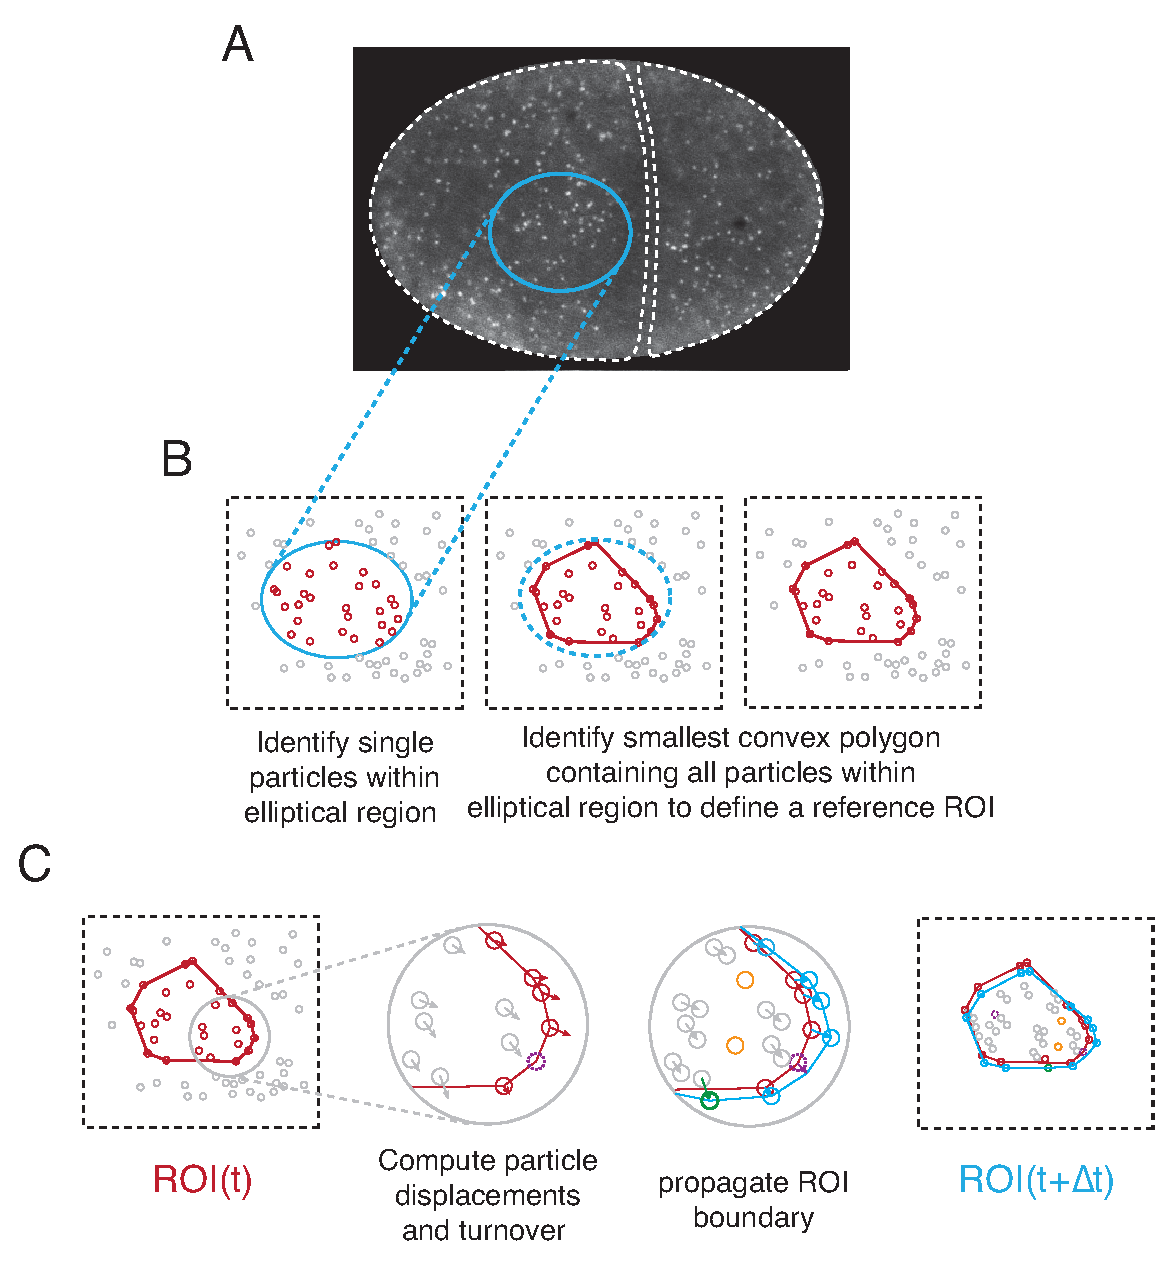
\includegraphics[width=0.8\textwidth]{Figure2-10}
\captionof{figure}[Schematic overview of methods for tracking a moving and deforming patch of cortex from single molecule data.]{\textbf{Schematic overview of methods for tracking a moving and deforming patch of cortex from single molecule data.} (A) Micrograph of a two-cell stage embryo expressing Actin::GFP at single-molecule levels. Anterior is to the left.  Dashed lines indicate the outlines of AB and P1.  The blue ellipse identifies a region in which a pulse occurs, from which a “reference ROI” will be extracted. (B) Method for extracting the reference ROI. Left:  Single particles detected in the raw image.  The particles shown in red are those contained within the blue ellipse.  Middle and right: The reference ROI (solid red line) is the smallest convex polygon containing all red particles. (C) Strategy for iterative propagation of the polygonal ROI from frame to frame (either backwards or forwards in time).  The polygon's vertices move with the particle that defined that vertex so long as the particle remains visible. When a particle associated with a vertex disappears (dashed magenta particle in middle left panel), the vertex displacement is extrapolated from the motion of the surrounding particles. If an internal particle moves outside the boundaries of the polygon defined by existing vertices (green particle in middle right panel) a new vertex associated with that particle is introduced.}
\end{figure}




%Figure 2.2.11

\begin{figure}[!htbp]
\centering
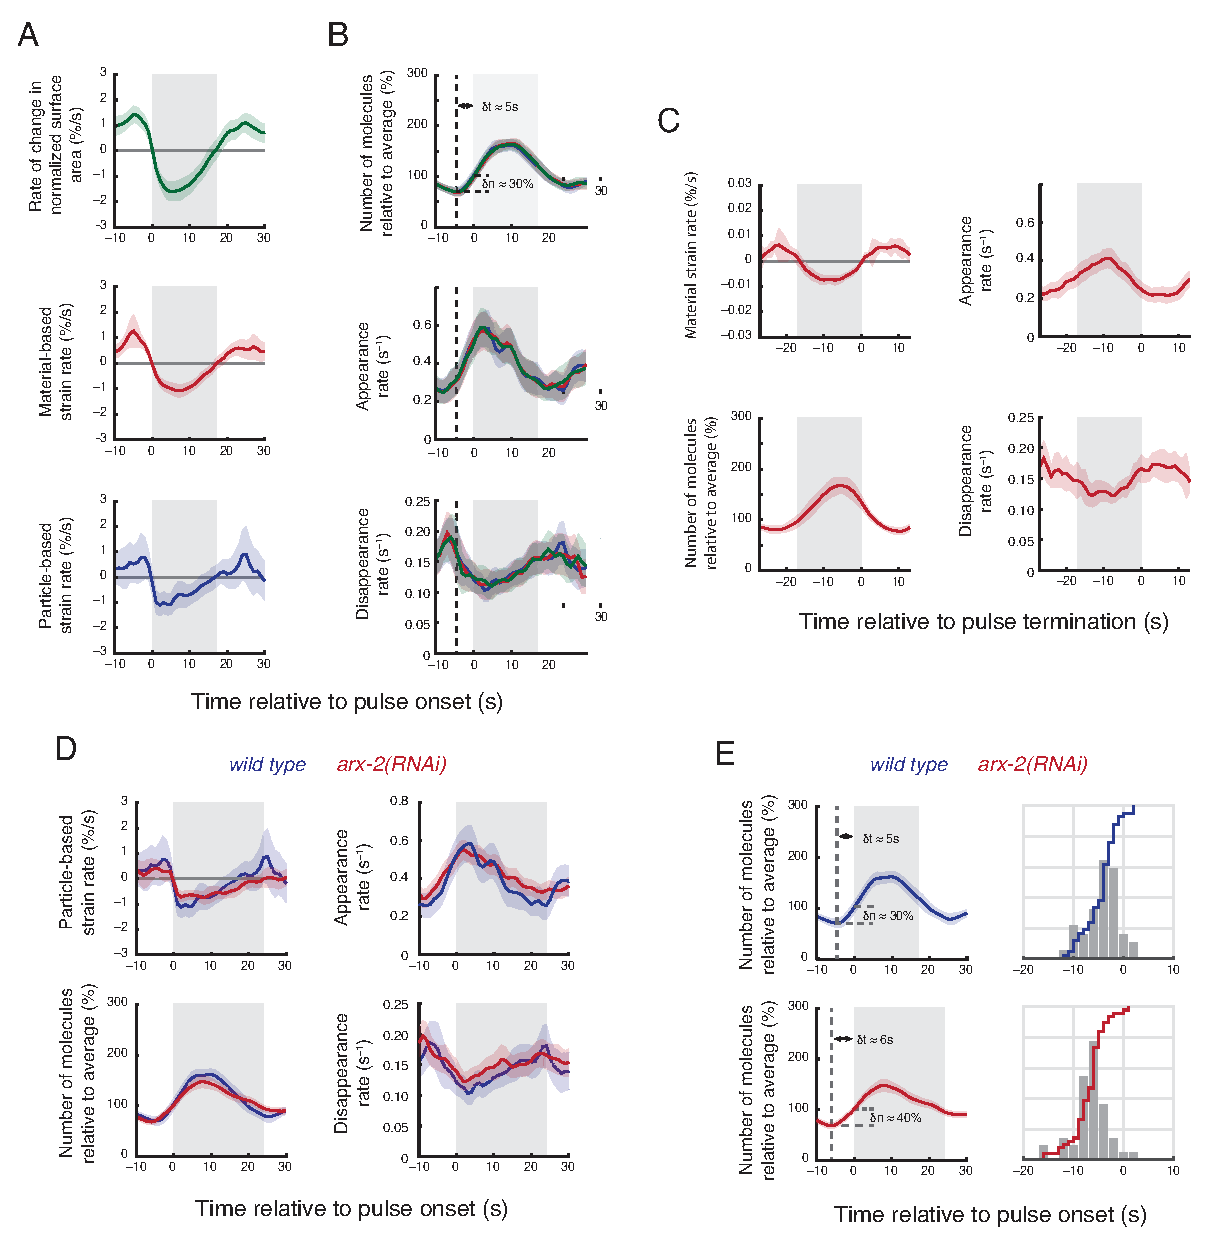
\includegraphics[width=0.8\textwidth]{Figure2-11}
\captionof{figure}[Comparison of different methods to quantify local deformation (strain rate) and to align data across multiple pulses.]{\textbf{Comparison of different methods to quantify local deformation (strain rate) and to align data across multiple pulses.} (A,B) Comparison of different methods used to compute local deformation rates during pulses. (A) Measures of deformation rate vs time for the same data using three different metrics: (top) Rate of change in normalized surface area, (middle) material strain rate and (bottom) particle based strain rate (see materials and methods for details on how these were computed). (B) Measurements of single molecule number (top), appearance rate (middle) and disappearance rate (bottom) were aligned and averaged with respect to the onset of contraction, over 42 pulses, using the three metrics to measure deformation: change in normalized surface area (green), material strain rate (red), and particle-based strain rate (blue). Vertical dashed lines mark lowest actin density preceding the pulse. Horizontal dashed lines in top graph mark, respectively, the minimum number of actin molecules and the number of molecules at the onset of contraction. For all three metrics, the delay from actin minimum to contraction onset is $\delta$t $\approx$ 5s, and the relative change in number of molecules from minimum to contraction onset is $\delta$n $\approx$ 30$\%$. (C) Measurements of material strain rate, number of molecules, appearance rate and disappearance rate, aligned and averaged with respect to the end of contraction for the same data shown in A&B. (D) Measurements of particle-based strain rate, number of molecules, appearance rate and disappearance rate, aligned and averaged with respect to the onset of contraction, in wild type (blue, n = 42 pulses) and \textit{arx-2}(RNAi) (red, n = 49 pulses) embryos. (E) Left column: number of molecules relative to average in wild type (blue) and \textit{arx-2}(RNAi) (red) embryos, as previously displayed in (D). The vertical dashed line marks lowest actin density preceding the pulse, delayed respectively by $\delta$t $\approx$ 5s and $\delta$t $\approx$ 6s from the contraction onset (gray box). The horizontal dashed line displays the amount of pre-contraction increase in the number of actin molecules, with $\delta$n $\approx$ 30$\%$ and $\delta$n $\approx$ 40$\%$, respectively. Right column: a histogram showing the distribution of delays between contraction onset and increase of actin molecules. Staircase line: cumulative distribution function of the delays. Error bars report 95$\%$ confidence intervals.}
\end{figure}







%Figure 2.2.12
\begin{figure}[!htbp]
\centering
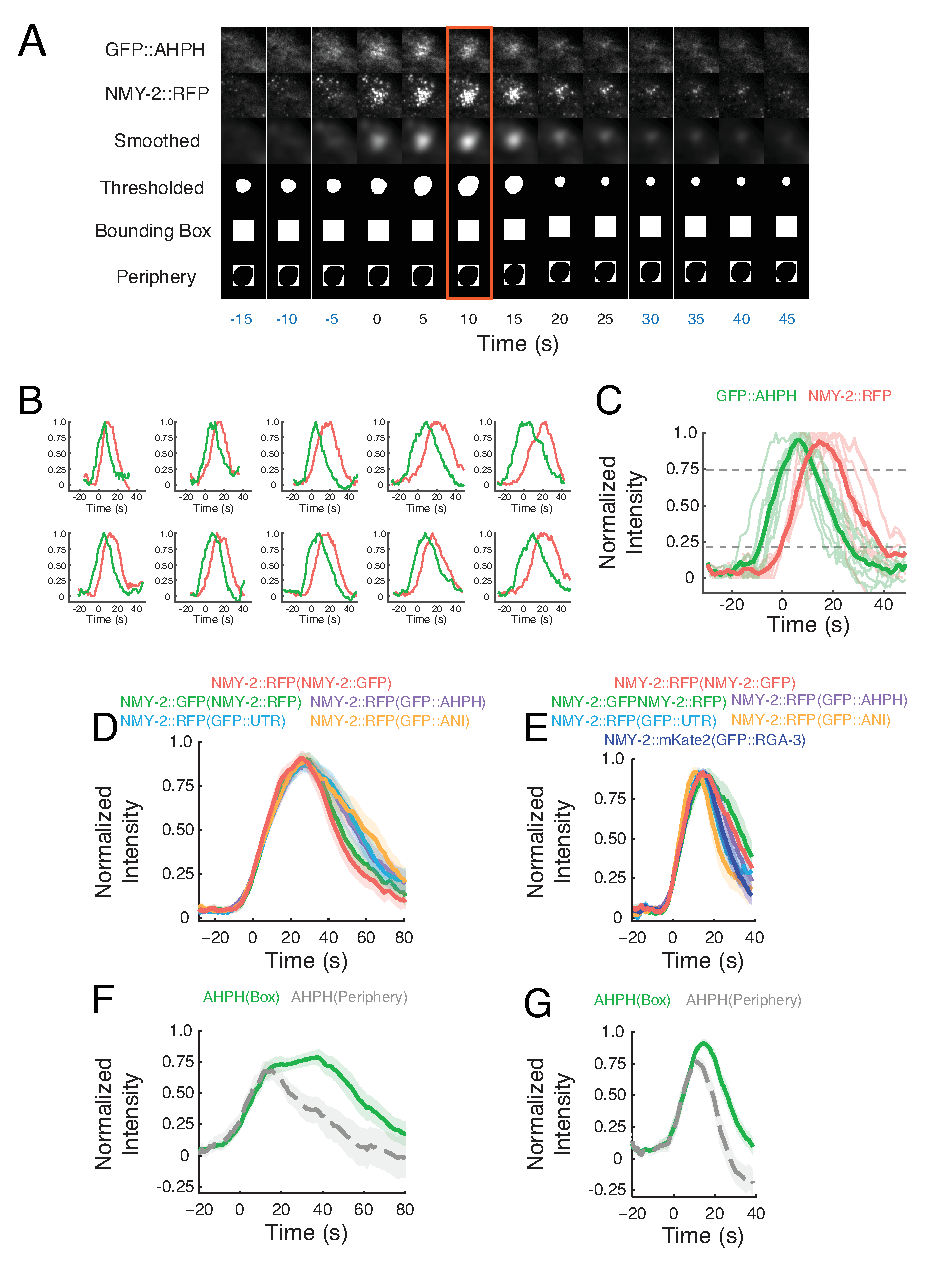
\includegraphics[width=0.7\textwidth]{Figure2-12}
\captionof{figure}[Schematic overview of methodology for measuring and aligning fluorescence intensities from two-color data during pulsed contractions.]{\textbf{Schematic overview of methodology for measuring and aligning fluorescence intensities from two-color data during pulsed contractions.} (A) Method for determining regions of interest in which to measure fluorescence intensities, illustrated for a single pulse.  Row 1:  raw GFP::AHPH signal. Row 2: raw NMY-2::RFP signal.  Row 3: smoothed NMY-2::RFP signal. Row 4: thresholded NMY-2::RFP signal. Row 5: The smallest box containing the largest thresholded domain is the bounding box.  In each frame, the center of bounding box is located on the centroid of the thresholded domain. Row 6: A fixed-size peripheral region is the complement of the largest thresholded region within its bounding box.      The center of the fixed-size peripheral region is located at the center of the thresholded region in each frame.  (B) Normalized fluorescence intensity of GFP::AHPH and NMY-2::RFP versus time for ten representative pulses in AB cells. Time t = 0 when NMY-2::RFP rises above 25$\%$ of its normalized maximum value. (C) Fluorescence intensities from all pulses in (B) co-aligned relative to time t = 0. The bold traces represent the average GFP::AHPH and NMY-2::RFP intensities. (D,E) Alignment of averaged normalized fluorescence intensities for NMY-2::XFP measured for pulses in P0 (D) and AB (E) cells co-expressing the indicated probes (shown in parentheses). Time t = 0 is when NMY-2::XFP rises above 25$\%$ of its normalized maximum value. (F,G) Averaged normalized fluorescence intensity of GFP::AHPH measured in the bounding box (green) and periphery (gray) for pulses in P0 (F) and AB (G) cells.  In (D-G), halos report 95$\%$ confidence intervals.}
\end{figure}
















%Figure 2.2.13
\begin{figure}[!htbp]
\centering
\includegraphics[width=0.8\textwidth]{Figure2-13}
\captionof{figure}[Two color analysis of Myosin II and Anillin dynamics during pulsed contractions in one- and two-cell embryos.]{\textbf{Two color analysis of Myosin II and Anillin dynamics during pulsed contractions in one- and two-cell embryos.}(A,E) Micrographs of two-cell (A) and one-cell (E) embryos co-expressing GFP::ANI-1 and NMY-2::RFP. White arrowheads indicate individual pulses. (B,F) Expanded views of single pulses illustrating temporal dynamics of GFP::ANI-1 and NMY-2::RFP accumulation. (C,G) Plots of averaged normalized fluorescence intensities for NMY-2::RFP and GFP::ANI-1 from two-color movies, aligned to the time at which NMY-2::RFP reaches 25$\%$ threshold. The averaged normalized fluorescence intensity of GFP::AHPH, co-aligned using the NMY-2::RFP signal, is shown for reference. Halos report 95$\%$ confidence intervals. (D,H) Distribution of the delays in the onset of appearance and disappearance of GFP::ANI-1 measured relative to NMY-2::RFP.  Onset of appearance and disappearance were measured respectively as the time at which the normalized signal rose above 25$\%$ or fell below 75$\%$ of the maximum value. }
\end{figure}




%Figure 2.2.14
\begin{figure}[!htbp]
\centering
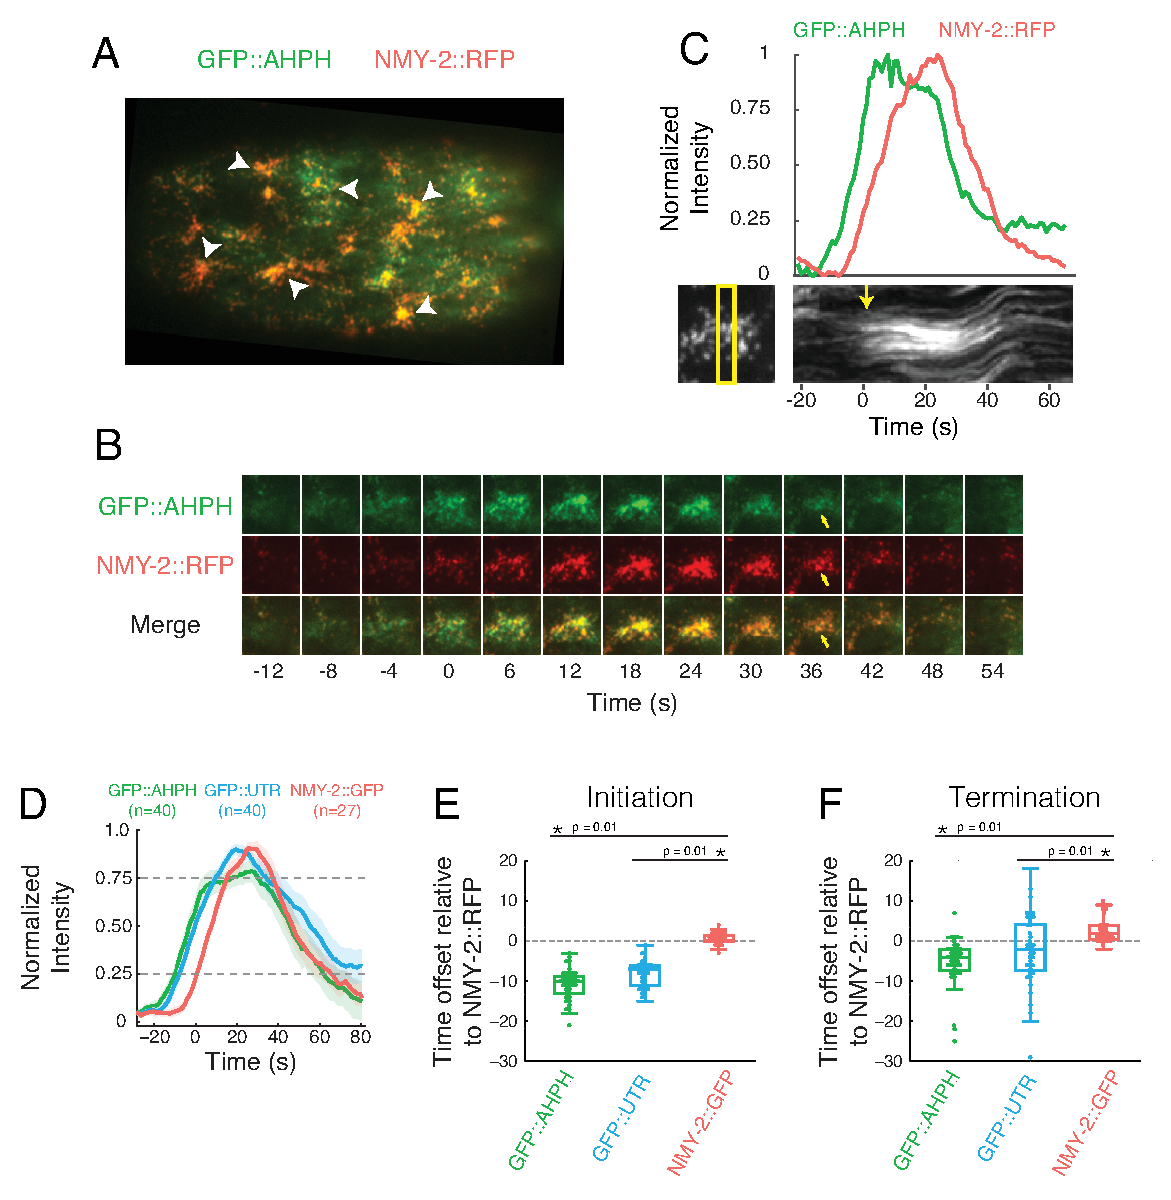
\includegraphics[width=0.9\textwidth]{Figure2-14}
\captionof{figure}[Two color analysis of pulsed contractions in P0.
]{\textbf{Two color analysis of pulsed contractions in P0.} (A) A zygote expressing GFP::AHPH and NMY-2::RFP. White arrowheads indicate individual pulses. (B) Expanded view of a single pulse illustrating temporal dynamics of GFP::AHPH and NMY-2::RFP accumulation. Time delay between frames is 4s for the first 4 frames, and 6s thereafter. (C) Plot of normalized fluorescence intensities of GFP::AHPH and NMY-2::RFP versus time for the pulse displayed in (B). Below: kymograph showing movements of NMY-2::RFP punctae before and during the pulse. Yellow box at left indicates the region used to make kymograph. Yellow arrow at right indicates the onset of contraction. Note that a sharp rise in GFP::AHPH precedes both Myosin accumulation and onset of contraction. (D) Averaged normalized fluorescence intensities for NMY-2::RFP, GFP::AHPH and GFP::UTR from two-color movies, aligned to the time at which NMY-2::RFP reaches 25$\%$ threshold. Halos report 95$\%$ confidence intervals. (E) Distributions of the delay in onset of accumulation of GFP::AHPH, GFP::UTR, and NMY-2::GFP, measured relative to the onset of accumulation of NMY-2::RFP during pulse initiation for many individual pulses. Onset of accumulation is measured as the time at which each normalized signal exceeds 25$\%$ of its maximum value. (F) Distributions of the delay in the onset of disappearance of GFP::AHPH, GFP::UTR, and NMY-2::GFP measured relative to NMY-2::RFP during pulse termination for many individual pulses. Onset of disappearance is measured as the time at which each normalized signal falls below 75$\%$ of its maximum value. In (E,F) box plots, the central mark represents the median, the box indicates the 25th and 75th percentile, the whiskers mark the minimum and maximum values and the ``+” symbol represents outliers.}
\end{figure}








\end{document}

\documentclass{ucetd}
\usepackage{subfigure,epsfig,amsfonts}
\usepackage{natbib}
\usepackage{amsmath}
\usepackage{amssymb}
\usepackage{amsthm}
\graphicspath{ {figures/ch3/} }
\begin{document}

\chapter{Effectors downstream of RhoA regulate pulse size and spatial dynamics}

\section{Abstract}
We have previously shown that pulsatile RhoA dynamics drive the initiation and termination of pulsed contractions in the early \textit{C.elegans} embryo.  We have shown that autocatalytic activation of RhoA precedes the assembly of F-actin, and activation of Myosin II, within pulsed contractions.  Inhibition of active RhoA, which is mediated by the redundant RhoA GAPs RGA-3 and RGA-4, precedes the disappearance of F-actin and Myosin II.  Although we understand many details about how pulsed contractions are regulated temporally, it is still unclear how pulses of active RhoA are regulated spatially.  The purpose of this chapter is to report some interesting observations that suggest that tuning effectors downstream of active RhoA plays a role in regulating spatial features of RhoA pulses such as size, lifetime, and the propensity to form traveling waves.


\section{Introduction}
Local activation of RhoA has been shown to be an important component of pulsed contractions during apical constriction during both mesoderm invagination and germ band extension in \textit{Drosophila} \cite{Mason:2013ee, Munjal:2015bx, Mason:2016bs}.  In \textit{C.elegans} embryos, autocatalytic activation of RhoA is thought to drive the accumulation of downstream factors such as F-actin, myosin II, and anillin during pulsed contractions (Figure 2.4, Figure 2.6).  RhoA promotes actin polymerization and myosin II activation through the activities of the formin CYK-1 and Rho kinase (LET-502), respectively (Figure 3.1).  Although it is unlikely that these downstream factors participate in a positive feedback with RhoA, it remains unclear how they might otherwise affect the spatial regulation of RhoA and contractile dynamics during pulsed contractions.  For example, RhoA continued to pulse in the absence of myosin II.  However, the \textit{nmy-2} RNAi pulses were qualitatively very different that wild-type pulses.  This observation raises the possibility that RhoA pulse dynamics are somehow linked to underlying actomyosin cytoskeleton.  Here, we have demonstrated that tuning effectors downstream of RhoA such as CYK-1, LET-502, and ANI-1 can affect RhoA spatial and temporal dynamics.  The purpose of this chapter is to describe and highlight these interesting phenotypes in order to provide an avenue for future research.
%Figure 3.1
\begin{figure}[!htbp]
\centering
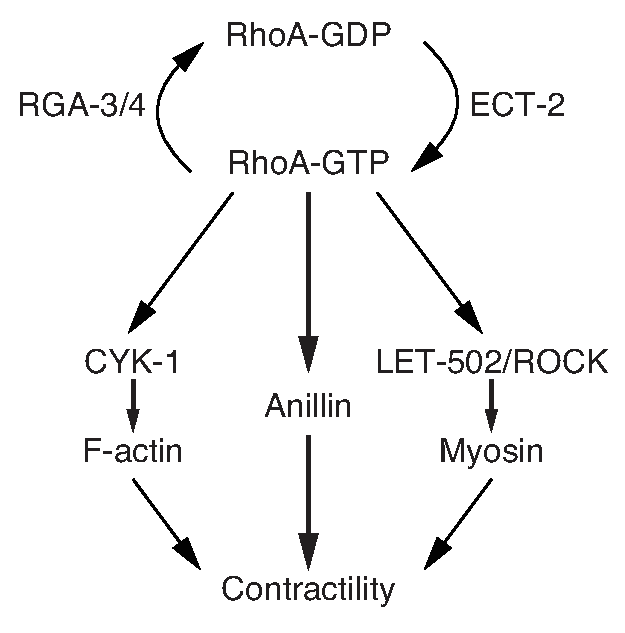
\includegraphics[width=0.45\textwidth]{Figure3-1}
\captionof{figure}[Excitable activation of RhoA drives pulsed contractility through its downstream effectors.]{\textbf{Excitable activation of RhoA drives pulsed contractility through its downstream effectors.} Local activation and deactivation of RhoA during pulsed contractions is regulated by the GEF ECT-2 and the Rho GAPs RGA-3/4, respectively. Active RhoA promotes actin polymerization through the activity of the formin CYK-1, and Myosin II activation through LET-502/ROCK.  The scaffold protein Anillin is thought to regulate pulsed contractions by stabilizing Myosin II. }
\end{figure}


\section{Results}
\subsection{RhoA does not pulse in the absence of an intact F-actin network}
Recent work from Bement \textit{et al.} has demonstrated that F-actin plays a role in negatively regulating excitable RhoA dynamics \cite{Bement:2015jp}.  In addition to playing a role as a scaffold, we hypothesize that F-actin facilitates negative feedback onto RhoA by recruiting the RhoA GAPs RGA-3 and RGA-4 during pulsed contractions in \textit{C.elegans}.  We have shown that RhoA does not pulse in the absence of RGA-3/4, but instead localizes uniformly to the cortex.  We have also shown that GFP::RGA-3 strongly co-localizes with mCherry::LifeAct on actin filaments in both P0 and AB.  Furthermore, we observed that RGA-3 does not localize to the cortex when embryos are treated with latrunculin A.  Therefore, we hypothesize that RhoA will uniformly localize to the cortex in the absence of an intact F-actin network.



To further test the idea that F-actin acts as a scaffold to promote negative feedback onto RhoA, we used latrunculin A to inhibit F-actin assembly in single-cell embryos.  Embryos were permeabilized by \textit{perm-1} RNAi and treated with 10$\mu$M latrunculin A \cite{Carvalho:2011ce}.  First, we tested whether myosin II or anillin continued to accumulate within pulses in the absence F-actin.  Upon latrunculin A treatment, we observed that GFP::ANI-1 and NMY-2::RFP did not pulse, but instead formed clusters in the absence of F-actin (Figure 3.2, top row).  Similarly, GFP::AHPH co-clustered with NMY-2::RFP in the absence of F-actin (Figure 3.2, bottom row).  These clusters were very stable, lasting the entire duration of polarity establishment (data not shown).  The clusters we observed are reminiscent of those observed by Hickson \textit{et al.} in \textit{Drosophila} S2 cells \cite{Hickson:2008hu}.  Hickson \textit{et al.} showed that anillin, myosin II, and septin all co-cluster when \textit{Drosophila} S2 cells are treated with latrunculin A during cytokinesis \cite{Hickson:2008hu}.  They also showed that the formation of these clusters was RhoA dependent and required the presence of anillin or septin \cite{Hickson:2008hu}.  These results reinforce the idea that an intact F-actin network is required for the proper recruitment of factors downstream of RhoA.

%Figure 3.2
\begin{figure}[!htbp]
\centering
\includegraphics[width=0.85\textwidth]{Figure3-2}
\captionof{figure}[Depolymerization of F-actin induces co-clustering of Myosin II, Anillin, and the active RhoA biosensor.]{\textbf{Depolymerization of F-actin induces co-clustering of Myosin II, Anillin, and the active RhoA biosensor.} Embryos co-expressing GFP::ANI-1 and NMY-2::RFP (top row) and embryos co-expressing GFP::AHPH and NMY-2::RFP (bottom row) were permeabilized by \textit{perm-1} RNAi treatment.  The addition of 10$\mu$M latrunculin A caused a complete loss of cortical F-actin and the formation of ectopic clusters containing Anillin, Myosin II, and the probe for active RhoA.}
\end{figure}

The above results suggest that RhoA does not pulse in the absence of F-actin.  However, it is possible that the RhoA biosensor accumulating within punctae is an artifact due to its ability to bind other factors through its PH domain.  To get around this, we attempted to inhibit the formation of these punctae by depolymerizing the actin cortex in a strain expressing the RhoA biosensor in a septin (UNC-59 in \textit{C.elegans}) mutant background.  In this experiment, we imaged embryos expressing GFP::AHPH before and after an acute latrunculin A treatment.  Prior to treatment, RhoA formed robust pulses on the cortex in both control and mutant embryos.  As expected, we observed the RhoA biosensor accumulate in stable punctae in control embryos in less than one minute after latrunculin A treatment (Figure 3.3, top row).  In contrast, the RhoA biosensor localized uniformly to the cortex in \textit{unc-59} mutant embryos (Figure 3.3, bottom row).  Therefore, RhoA pulses requires an intact F-actin network.
%Figure 3.3
\begin{figure}[!htbp]
\centering
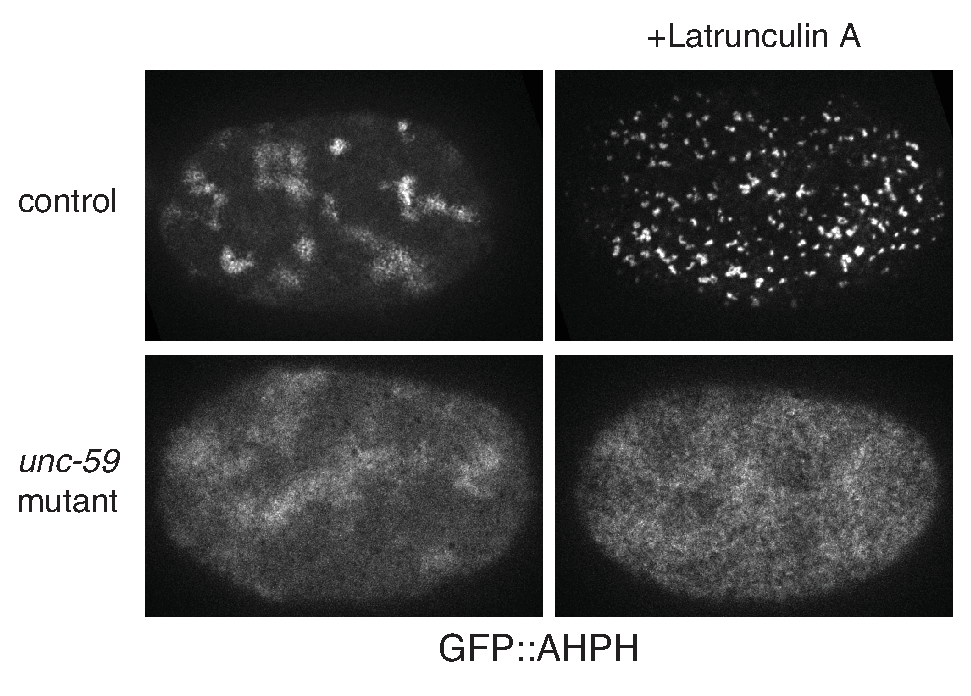
\includegraphics[width=0.65\textwidth]{Figure3-3}
\captionof{figure}[Septin mediates clustering of the active RhoA biosensor in latrunculin A treated embryos.]{\textbf{Septin mediates clustering of the active RhoA biosensor in latrunculin A treated embryos.]} Control and \textit{unc-59} mutant embryos expressing GFP::AHPH were acutely treated with 10$\mu$M latrunculin A.  In control embryos, the active RhoA biosensor formed clusters that contained Anillin and Myosin II (Figure 3.2).  In mutant embryos, active RhoA did not form clusters, but instead localized uniformly on the cortex.}
\end{figure}

\subsection{Depletion of CYK-1 affects RhoA pulse size, duration, and spatial distribution}

%cyk-1
Our previous experiments have robustly demonstrated that pulsatile RhoA activity drives pulsed contractions in \textit{C.elegans}, and that RhoA pulses do not rely on the presence of myosin II or myosin II-dependent contractility.  The fact that active RhoA does not locally pulse in the absence of F-actin, but instead localizes uniformly to the cortex, suggests that actomyosin dynamics might play role in shaping RhoA pulses.  To test this idea, we've used RNAi to mildly deplete key effectors downstream of active RhoA.  In order to compare the different phenotypes, we tracked the GFP::AHPH signal for multiple pulses, and aligned their normalized intensities relative to the time point at which GFP::AHPH reaches 25$\%$ its maximum intensity (Figure 3.5).  We also present kymographs to compare RhoA spatial dynamics.


First, we targeted the major \textit{C.elegans} formin CYK-1 \cite{Swan:1998tv}.  CYK-1, together with profilin (PFN-1 in \textit{C.elegans}) was shown to mediate the polymerization of actin filaments independent of the ARP-2/3 complex \cite{Severson:2002ve}.  Severson \textit{et al.} also showed that CYK-1 mediated actin polymerization is necessary for A-P polarity establishment as well as cytokinesis in the early embryo.  We imaged embryos co-expressing GFP::AHPH and NMY-2::RFP under conditions in which the formin CYK-1 was mildly depleted by RNAi.  RhoA and myosin II strongly co-localized within punctae within pulsed contractions as well as other regions of the cortex.  The averaged intensity profile shows that RhoA accumulates with similar kinetics in \textit{cyk-1} depleted embryos compared to wild-type embryos (Figure 3.5A).  In contrast, the duration of \textit{cyk-1} RNAi pulses appears shorter than wild-type P0 pulses (Figure 3.5A).
%Figure 3.4
\begin{figure}[!htbp]
\centering
\includegraphics[width=0.95\textwidth]{Figure3-4}
\captionof{figure}[Depletion of RhoA effectors changes RhoA spatial dynamics.]{\textbf{Depletion of RhoA effectors changes RhoA spatial dynamics.} Micrographs of single-cell P0 embryos co-expressing GFP::AHPH (top panels) and NMY-2::RFP (middle panels) under various conditions.  Pulses in \textit{cyk-1}, \textit{let-502}, and \textit{ani-1} RNAi embryos appeared larger than pulses in wild-type embryos.  (Bottom panels) The dashed yellow box indicates the region of each micrograph in the top panels used to make the kymograph.  The kymographs reveal a decrease in cortical flow in \textit{cyk-1}, \textit{let-502}, and \textit{ani-1} RNAi embryos compared to wild-type embryos.  Pulses in \textit{cyk-1} and \textit{ani-1} RNAi embryos appear to have a shorter duration than wild-type and \textit{let-502} embryos.}
\end{figure}

We also observed that RhoA pulses appeared spatially larger in \textit{cyk-1} depleted embryos than in wild-type embryos (Figure 3.4, first and second  columns).  We quantified this by measuring the ratio of the size of RhoA pulses relative to the size of the embryo in which they were observed (Figure 3.5B).  On average, \textit{cyk-1} RNAi pulses were about 6$\%$ the size of the embryo, while wild-type pulses were about 2.5$\%$ the size of the embryo.  A visual inspection of \textit{cyk-1} depleted embryos suggests that fewer RhoA pulses form on the cortex an any given time.  A comparison of kymographs from representative wild-type and \textit{cyk-1} depleted embryos shows a decrease in cortical flow in \textit{cyk-1} embryos during polarity establishment.  These data suggest that CYK-1-mediated actin assembly plays a role in regulating RhoA spatial dynamics.

\subsection{Depletion of LET-502 affects RhoA pulse size and spatial dynamics}
%let-502
Our previous results support the idea that RhoA pulses are independent of myosin II (see Chapter 2).  However, in the absence of myosin II RhoA pulses were qualitatively and quantitatively different than pulses in wild-type pulses.  The \textit{nmy-2} RNAi pulses appeared weaker, and also shorter than wild-type pulses.  Munjal \textit{et al.} showed that inhibiting Rho kinase (Rok in \textit{Drosophila}, LET-502 in \textit{C.elegans}) with the inhibitor Y27632 abolished RhoA pulses, as well as blocked the cortical recruitment of other factors involved in pulsed contractions during germband extension \cite{Munjal:2015bx}.  Therefore, we wondered if depleting LET-502 would weaken RhoA pulses or completely eliminate them.  As expected, there was a marked decrease in myosin II both on the cortex and within pulsed contractions (Figure 3.4, third column).  We also observed a decrease in cortical flow during polarity establishment (Figure 3.4, third column).  These results are consistent with LET-502 being a key activator of myosin II activity.  Surprisingly, however,  RhoA continued to pulse robustly under strong \textit{let-502} RNAi conditions (Figure 3.4, third column).  Similar to \textit{cyk-1} RNAi pulses, \textit{let-502} RNAi pulses were also larger than wild-type P0 pulses (Figure 3.5B).  Furthermore, \textit{let-502} RNAi pulses showed an increased propensity for forming traveling waves.  Although \textit{let-502} RNAi pulses exhibited different spatial dynamics than wild-type pulses, the initiation and termination kinetics appear similar to wild-type P0 pulses.  Therefore, strong depletion of LET-502 does not inhibit RhoA pulses, but instead alters RhoA pulse size and spatial dynamics.




\subsection{Depletion of ANI-1 affects RhoA pulse size and duration}
%ani-1
Anillin (ANI-1 in \textit{C.elegans}) is a scaffold protein that plays an important role in regulating actomyosin contractility during cytokinesis in human and \textit{Drosophila} cells \cite{Piekny:2010es}.  It is thought to bind F-actin, myosin II, septins, ECT-2, RhoA and other proteins \cite{Piekny:2010es}.  Maddox \textit{et al.} showed that ANI-1 plays a role in polar body extrusion, asymmetric cell division, and cortical ruffling (i.e., pulsed contractions) and pseudocleavage during polarity establishment \cite{Maddox:2005gd}.  They reported a nearly complete loss of myosin II pulses in P0 under strong \textit{ani-1} RNAi conditions \cite{Maddox:2005gd}.  Under these conditions, myosin II localizes uniformly to the cortex instead of in dense foci.  In contrast, ANI-1 patches remained on the cortex in the absence of myosin II.  The authors proposed that ANI-1-mediated positive feedback drives pulsed contractions by binding and \cite{Maddox:2005gd}.  In their model, ANI-1 is recruited locally to the cortex through its PH- and actin-binding domains, where ANI-1 then promotes its own accumulation by recruiting F-actin.

We have shown that the accumulation of RhoA within pulsed contractions is autocatalytic, and that activate RhoA precedes the accumulation of F-actin, myosin II, and anillin within pulsed contractions (see Chapter 2).  Although our results argue against anillin initiating pulsed contractions, it is still not clear how anillin might affect RhoA dynamics during pulsed contractions.  To test this, embryos expressing the active RhoA biosensor and NMY-2::RFP were depleted of ANI-1 via RNAi.  Since the biosensor is made from a fragment of ANI-1, we used RNAi targeting anillin's myosin binding domain.  The \textit{ani-1 (myo)} RNAi phenotype was characterized by a loss of pseudoclavage and a decrease in cortical flow (Figure 3.4, fourth column).  Although RhoA and myosin II still accumulated in pulses, myosin II did not form dense foci similar to pulsed contractions in wild-type embryos.  Similar to the \textit{cyk-1} RNAi phenotype, \textit{ani-1 (myo)} RNAi pulses were larger than P0 pulses (Figure 3.5B).  Furthermore, \textit{ani-1 (myo)} RNAi appeared to be shorter in duration than P0 pulses (Figure 3.5A).  Taken together, these results suggest that ANI-1 might play a role in stabilizing myosin II within pulsed contractions as well as limiting the size of RhoA pulses.

%Figure 3.5
\begin{figure}[!htbp]
\centering
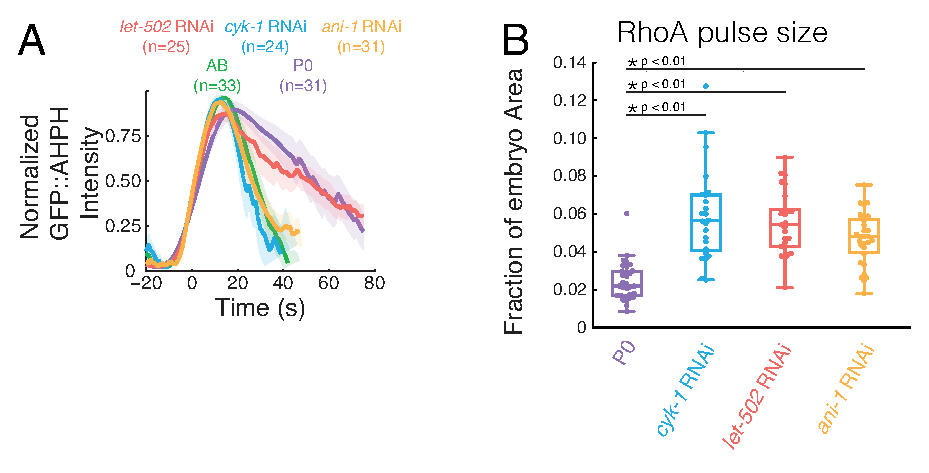
\includegraphics[width=0.85\textwidth]{Figure3-5}
\captionof{figure}[Quantification of RhoA pulse size and duration.]{\textbf{Quantification of RhoA pulse size and duration.} (A) Comparison of averaged normalized fluorescence intensities vs time for active RhoA (GFP::AHPH).  Data were co-aligned with respect to the time at which GFP::AHPH reaches 25$\%$ threshold. Hued regions report 95$\%$ confidence intervals. (B) Knocking down various RhoA effectors changes the size of RhoA pulses.  The size of each RhoA pulse was measured at the time at which GFP::AHPH fluorescence intensity reached its max.  Each measurement was normalized by the area of the embryo in which the pulse occured. }
\end{figure}


Although our results argue against the model proposed by Maddox \textit{et al.}, we have not ruled out the possibility that anillin is required for RhoA pulses.  This is largely due to the inefficiency of knocking down ANI-1 when targeting its myosin binding domain.  To get around this, we wanted to use RNAi to target full length ANI-1 in embryos co-expressing NMY-2::RFP and  fully labeled GFP::LET-502 (made by Thanh Vuong, Labouesse lab).  As a control, we compared embryos expressing GFP::LET-502 to embryos expressing GFP::AHPH.  In wild-type embryos, LET-502's distribution on the cortex is reminiscent of the RhoA biosensor (Figure 3.4 and Figure 3.6).  LET-502 also co-localizes with NMY-2::RFP within pulsed contractions (Figure 3.6, first column).   In order to confirm that the accumulation of LET-502 on the cortex is RhoA dependent, we used RNAi to partially knockdown RhoA (RHO-1 in \textit{C.elegans}).  We observed a strong decrease in cortical GFP::LET-502 during polarity establishment in \textit{rho-1} RNAi embryos (Figure 3.6, second column).  Consistent with this phenotype, partial \textit{rho-1} RNAi embryos also exhibited a decrease in cortical NMY-2::RFP and pulsed contractions (Figure 3.6, second column).  These data suggest that full-length GFP::LET-502 can be used as an alternate biosensor for detecting active RhoA on the cortex.


Thus, to determine if RhoA continues to pulse in the absence of ANI-1 we treated embryos co-expressing GFP::LET-502 and NMY-2::RFP with RNAi targeting ANI-1.  As expected, \textit{ani-1} RNAi embryos did not form a pseudocleavage furrow (Figure 3.6, third column).  We also observed a strong decrease in NMY-2::RFP pulse formation.  Interestingly, we did not observe a complete loss of myosin II pulses as reported by Maddox \textit{et al.} \cite{Maddox:2005gd}.  NMY-2::RFP did not accumulate in dense foci that correspond to deep membrane invaginations like in wild-type embryos (Figure 3.6, third column).  Instead NMY-2::RFP accumulated in transient pulses that appeared much weaker and shorter than wild-type pulses.  Our observations seem to contradict those reported by Maddox \textit{et al.}.  However, a close inspection of their supplemental movie data shows GFP::NMY-2 forming transient pulses during polarity establishment under strong \textit{ani-1} RNAi conditions \cite{Maddox:2005gd}.  We also observed that GFP::LET-502 continued to form robust pulses in the absence of ANI-1.  Control embryos co-expressing GFP::ANI-1 and NMY-2::RFP showed a drastic decrease in GFP::ANI-1 fluorescence intensity under \textit{ani-1} RNAi conditions (See Chapter 2, Figure 3.6, fourth column).  Together, these results suggest that although anillin is not required for RhoA pulses, it may play an important role in spatially regulating pulsed contractions.

%Figure 3.6
\begin{figure}[!htbp]
\centering
\includegraphics[width=0.95\textwidth]{Figure3-6}
\captionof{figure}[Rho kinase pulses in the absence of Anillin.]{\textbf{Rho kinase pulses in the absence of Anillin.} Micrographs of single-cell P0 embryos co-expressing GFP::LET-502 or GFP::ANI-1 (top panels) and NMY-2::RFP (middle panels) under various conditions.  (Bottom panels) The dashed yellow box indicates the region of each micrograph in the top panels used to make the kymograph.  (First column) wild-type GFP::LET-502 spatial dynamics are similar to the active RhoA biosensor.  (Second column) GFP::LET-502 does not accumulate on the cortex in partial \textit{rho-1} RNAi embryos. The kymograph shows cortical flows are still present in partial \textit{rho-1} RNAi embryos.  (Third column) GFP::LET-502 forms pulses under strong \textit{ani-1} RNAi conditions.  (Fourth column) Strong loss of fluorescence in control embryos co-expressing GFP::ANI-1 and NMY-2::RFP is indicative of a strong \textit{ani-1} RNAi phenotype..}
\end{figure}

\section{Discussion}
The work presented in this chapter demonstrates that RhoA pulses are not completely independent from the activity and dynamics of RhoA effector proteins.  We have shown that depolymerizing F-actin with latrunculin A completely eliminates RhoA pulsing (Figure 3.3).  Instead, RhoA localized uniformly to the cortex in the absence of F-actin.  This result recapitulates our previous result in which RhoA no longer pulses in the \textit{rga3/4} mutant background  (Figure 2.7).  Together, these results are consistent with our current working model, in which RhoA-dependent F-actin polymerization promotes the delayed accumulation of the Rho GAPs RGA-3 and RGA-4 that turns RhoA activity off (Figure 2.9).

The fact that RhoA does not pulse in the absence of an intact F-actin network raises the possibility that tuning the concentration of various regulators of the actomyosin cytoskeleton might alter RhoA dynamics in space or time.  We have shown that mild depletion of the formin CYK-1 disrupts RhoA spatial patterning, as well as causes RhoA pulses to become larger spatially, and shorter temporally.  Surprisingly, we also observed an increase in RhoA pulse size following the depletion Rho kinase.  In addition, we observed that RhoA pulses have a tendency to form traveling waves when Rho kinase is depleted.  This is in contrast to \textit{nmy-2} RNAi pulses, which appeared to oscillate and have a size similar to wild-type pulses.  These observations suggest that Rho kinase regulates RhoA dynamics independent of myosin II.  For example, it is possible that direct interactions between RhoA and Rho kinase prevent RhoA from spreading to nearby regions of the cortex.  Lastly, we observed a decrease in the lifetime of RhoA and myosin II pulses in the absence of anillin, even though LET-502 continued to form pulses on the cortex.  This suggest that anillin plays a role in recruiting and/or stabilizing myosin II on the cortex.  Taken together, the results presented in this chapter suggest that RhoA pulses are an emergent phenomenon, and their dynamics rely heavily on the structure and dynamics of the underlying actomyosin cytoskeleton.  Although the mechanism for generating RhoA pulses is still unclear, we believe that the phenotypes presented here will provide exciting avenues for future experiments (see Chapter 4).


\section{Materials and Methods}
For information about \textit{C.elegans} culture and strains, microscopy, pulse tracking and analysis, and kymograph analysis please refer to the materials and methods section of Chapter 2.

\subsection{RNA Interference}
RNA interference was performed by a well established feeding method \cite{Timmons:2001wg}.  Bacteria targeting \textit{spd-5}, \textit{perm-1}, \textit{ani-1} (Full length), \textit{rho-1}, \textit{let-502}, \textit{cyk-1} were obtained from the Kamath feeding library \cite{Kamath:2003bk}.  The \textit{ani-1} (myo) RNAi feeding strain that targets Anillin's myosin binding domain was a kind gift from the Glotzer lab.  For the experiments involving \textit{spd-5}, L4 larvae were transferred to \textit{spd-5} RNAi feeding plates for 24-30 hours before imaging.  For the latrunculin A experiments, late-stage L4 larvae were transfered to \textit{perm-1} RNAi feeding plates for 12-16 hours before imaging.  For the Anillin RNAi experiments, late-stage L4 larvae were transferred to \textit{ani-1} (full length) or \textit{ani-1} (myo) RNAI feeding plates for \(>\)  30 hours.  In the \textit{ani-1} (full length) experiments, A strong phenotype was verified in embryos co-expressing GFP::ANI-1 and NMY-2::RFP as a strong loss of GFP fluorescence, loss of pseudocleavage furrow formation, and the presence of transient NMY-2::RFP pulses.  The loss of pseudocleavage and the pattern of transient NMY-2::RFP pulses was used to assess the strength of the \textit{ani-1} phenotype in embryos co-expressing GFP::LET-502 and NMY-2::RFP.  For the RhoA experiments, young adults were transferred to \textit{rho-1} RNAi feeding plates 10-16 hours before imaging.  For experiments involving \textit{let-502} or \textit{cyk-1} RNAi, late-stage L4 larvae were transferred to feeding plates 24-30 hours before imaging.

\subsection{RhoA pulse size analysis}

RhoA (GFP::AHPH) pulses from  were detected, tracked, and analyzed as described in Chapter 2.  In order to measure the size of a RhoA pulse, we first extracted the size of the binary mask at the time RhoA reached its peak intensity.  We then segmented (by hand) the embryo that each pulse originated from and created a binary mask.  The area of the pulse mask and embryo mask were computed using built in MATLAB functions.  The pulse areas reported in the text and Figure 3.5 represent the ratio between the area of the pulse mask to the area of the embryo mask.


\end{document}

\documentclass{ucetd}
\usepackage{subfigure,epsfig,amsfonts}
\usepackage{natbib}
\usepackage{amsmath}
\usepackage{amssymb}
\usepackage{amsthm}
\graphicspath{ {figures/ch4/} }
\begin{document}
\chapter{Discussion}















\section{Summary}
%State of the field
Pulsed contractility is an increasingly common form of actomyosin contractility that is thought to play an important role in driving cell shape changes and tissue morphogenesis during development \cite{Gorfinkiel:2016bv}.  Pulsed contractions have been well characterized in \textit{Drosophila} tissues where they drive apical constriction of epithelial cells \cite{Rauzi:2011bk}.  On a subcellular level, pulsed contractions are characterized by cycles of local actomyosin assembly, contraction-mediated shape changes, and disassembly.  However, the mechanisms governing the initiation, termination, and spatial organization of pulsed contractions remain unclear.  One current model, known as the contractile instability model, postulates that pulsed contractions are initiated when local myosin II activity is self-amplified by the contraction-mediated accumulation of F-actin, Myosin II, and/or their upstream regulators (Figure 1.4) \cite{Bois:2011kx, Kumar:2014ux}.  Pulsed contractions terminate when either: i) Myosin II contractility promotes local network disassembly or ii.) tension built up within the network resists further deformation.  An alternate clustering model argues that pulsed contractions are initiated by mutual binding interactions between factors such Anillin and F-actin organize the cortex into patches has also been proposed \cite{Maddox:2005gd}.  A variant of this clustering model might involve Anillin positively feeding back onto RhoA directly, or indirectly through interactions with the GEF ECT-2 \cite{Piekny:2008jf, Frenette:2012do}. 

%My results
Here, we have definitively ruled out the contractile instability and clustering models as major mechanisms for initiating pulsed contractions in \textit{C.elegans}.  Instead, we propose a model in which local cycles of autocatalytic RhoA activation and delayed inhibition set the timing of actomyosin assembly, contraction, and disassembly within pulsed contractions.  We have shown that active RhoA begins to accumulate within pulsed contractions before downstream factors such as F-actin, Myosin II, and Anillin (Figure 2.4).  Our measurements reveal that active RhoA reaches a peak, and then begins to dissipate, before these factor as well (Figure 2.4).  Inconsistent with the contractile instability or clustering models, RhoA continues to pulse in the absence of Myosin II or Anillin (Figure 2.5, Figure 3.4).  We have established that the localization and dynamics of the Rho GAPs RGA-3/4 is consistent with their role in providing delayed negative feedback onto RhoA: GFP::RGA-3 accumulates with a delay relative to active RhoA and the deletion of RGA-3 and RGA-4 eliminates RhoA pulses (Figure 2.7).  Furthermore, we have established a potential mechanism for delayed inhibition of RhoA through F-actin-mediated recruitment of RGA-3/4 to the cortex.


%Figure 4.1
\begin{figure}[!htbp]
\centering
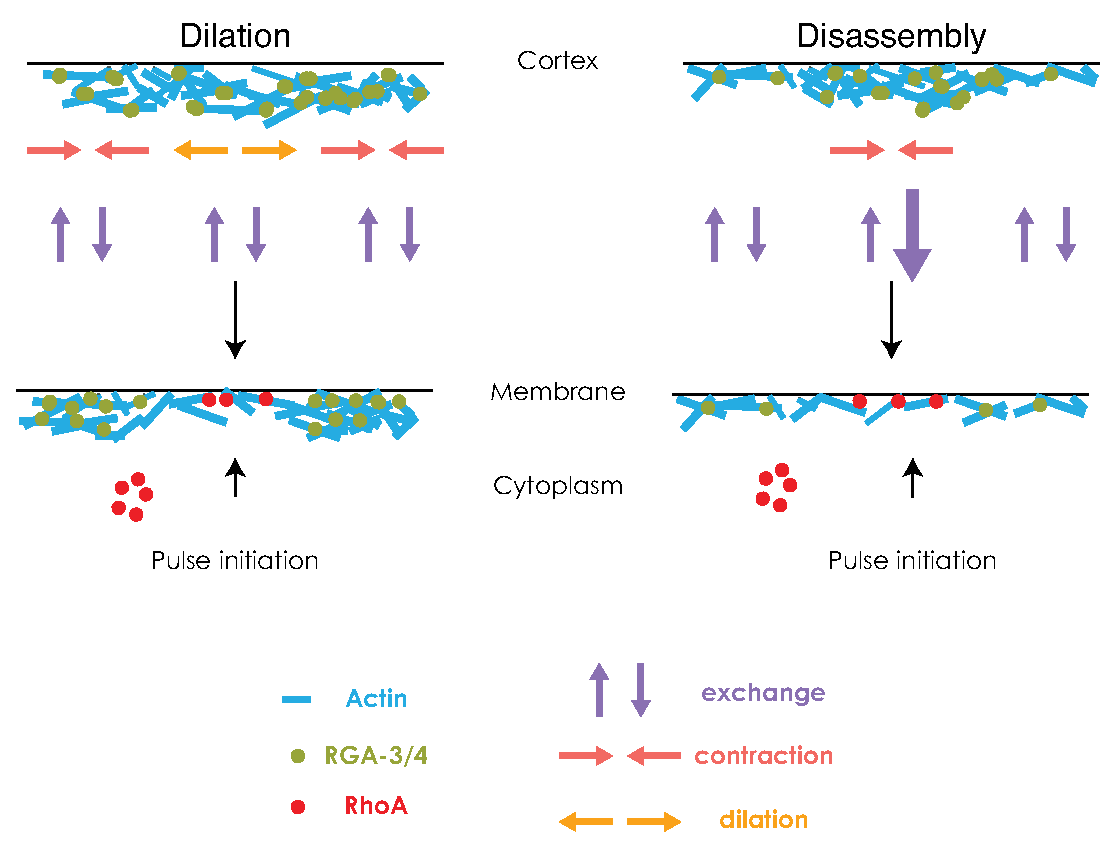
\includegraphics[width=\textwidth]{Figure4-1}
\captionof{figure}[Schematic of our novel conceptual model.]{\textbf{Schematic of our novel conceptual model.} Local pulses of active RhoA (red circles) can be triggered by a dilation (orange arrows) in the cortex (left) or local disassembly of actin filaments (cyan rods) (right).  Both dilation and disassembly lead to a decrease in F-actin, which in turn decreases RGA-3/4 (green circle) localization on the cortex.  In this model, local actin disassembly driven by myosin-mediated contractility (pink arrows).}
\end{figure}

\section{Proposed mechanism} 
Together, our results provide the basis for a novel mechanism for explaining pulsed contractions in particular, and cell shape changes in general.  In our current model, pulsed contractions are driven by autocatalytic activation of RhoA and terminated by the delayed recruitment of RGA-3/4 (Figure 2.9).  It is likely that we can rule out classic activator-inhibitor models in which pattern formation relies on long-range inhibition by a rapidly diffusing inhibitor \cite{Gierer:1972vq}.  Indeed, we have made two key observations.  First, the fact that GFP::RGA-3 strongly co-localizes with F-actin suggests that RGA-3 does not diffuse rapidly within the membrane (Figure 2.8).  Second, the depolymerization of F-actin leads to a rapid loss of GFP::RGA-3 on the cortex, and global activation of RhoA on the membrane (Figure 2.8).  We can therefore extend our model by considering how coupling RGA-3/4 activity to F-actin polymerization might spatiotemporally regulate RhoA activation and pulsed contraction dynamics.  Thus, a new model should contain the essential ingredients for an excitable system that exhibits spatial dynamics: the activator (RhoA) is autocatalytic, the inhibitor (RGA-3/4) provides delayed negative feedback, and the localization of inhibitor everywhere on the cortex ensures long-range inhibition.  Therefore, in order for RhoA to pulse on and off the cortex, stochastic fluctuations in active RhoA must exceed a threshold, or RGA-3/4 levels must locally decrease.  


%Local depletion of RGA-3/4
In principle, local RGA-3/4 levels could be modulated by dynamic changes of the underlying actin cytoskeleton.  In one scenario, local F-actin disassembly could lead to a decrease in RGA-3/4 levels, which could then promote the local accumulation of active RhoA (Figure 4.1).  We have often observed oscillations of pulsed contractions in AB embryos.  This observation is consistent with what our new model would predict: cycles of RhoA pulses are initiated by contraction-driven actin disassembly from the previous pulsed contraction.  Indeed, our single molecule measurements indicate that pulsed contractions are characterized by an increase in actin assembly during the initiation phase, and an increase in actin disassembly during the termination phase (Figure 2.3C,D).  In another scenario, large variations in contractility could drive tearing/dilations in the cortex (Figure 4.1).  A RhoA pulse would then form in the region that has been recently depleted of actin filaments.  Our preliminary observations suggests that multiple contracting pulses in close proximity could build up enough tension within the network to rupture nearby actin filaments, and promote the formation of a new pulsed contractions (Figure 4.2).  

%Figure 4.2
\begin{figure}[!htbp]
\centering
\includegraphics[width=0.85\textwidth]{Figure4-2}
\captionof{figure}[Myosin II pulses form in cortical regions depleted of RGA-3/4.]{\textbf{Myosin II pulses form in cortical regions depleted of RGA-3/4.} Micrograph of 1-cell stage embryo expressing GFP::RGA-3 and NMY-2::mKate.  The yellow arrowhead identifies a new pulsed contraction forming between two existing pulses.}
\end{figure}


%Model predictions
Although this model is currently speculative, it could in principle recapitulate all of our preliminary and well-established observations.  For example, this model would predict that global depletion of F-actin (or RGA-3/4) would lead to global activation of RhoA (Figure 2.7 and Figure 3.3).  This model would also predict that pulsed contractions are often preceded by local dilations in the cortex.  Indeed, our single molecule measurements indicate that the initiation of pulses often correlates with a dilation of the cortex (Figure 2.3G).  Furthermore, we would expect that perturbations that decrease the polymerization rate, or stability, of actin filaments to promote larger tears in the cortex pulses, and hence larger pulses.  Consistent with this prediction, we have observed larger pulses in \textit{cyk-1} (and \textit{pfn-1}) RNAi embryos in which local cortical dynamics are exaggerated relative to wild-type embryos (Figure 3.4, Figure 3.5).  Similarly, we would expect that perturbations that stabilize the actin cortex should either decrease the amplitude or duration of pulses, or eliminate them altogether.  For example, our observations suggest that RhoA pulses in \textit{nmy-2} RNAi embryos are not as robust as wild-type pulses, and they appear to terminate more rapidly.  Consistent with this result, we have observed that stabilizing actin filaments with the drug jasplakinolide also dampens active RhoA pulses (data not shown).  Thus, our new model provides a novel conceptual framework that has the capacity to explain our previous experimental results, as well as guide future experiments.



\section{Open Questions}
%How do you get different RhoA pulse dynamics
Although we have gained key insights into the mechanisms regulating pulsed contractility, many details of pulsed contractions are still not well understood.  For example, we currently understand very little about how pulsed contractions are regulated spatially.  What determines the size of a pulse?  Where is a pulsed contraction most likely to form on the cortex?  To what extent are neighboring pulses coupled?  What regulates the overall spatial pattern of pulsed contractions on the cortex?  Answering these questions might help to uncover, for example, why pulsed contractions in P0 embryos are different than pulsed contractions in AB embryos.  The cortex of P0 embryos is highly stereotyped, where pulses maintain a characteristic size and spacing throughout polarity establishment \cite{Munro:2004jk}.  In contrast, the size, number, and pattern of pulses in AB is much more variable.  In some AB embryos, pulsed contractions may oscillate in one region of the cortex for multiple cycles.  In other AB embryos, pulsed contractions that appear to be organized randomly on the cortex will be highly synchronized temporally, where each pulse initiates and terminates simultaneously.  Is RhoA locally activated in multiple cortical regions simultaneously?  Or, is RhoA globally activated?  How, then, would RhoA effectors spatially segregate into different pulses instead of forming one large pulse?  Other key differences between P0 and AB pulses are their duration and the extent to which they contract.  P0 pulses tend to be longer in duration and form deeper membrane invaginations than AB pulses.  This is surprising, as the initial kinetics of active RhoA accumulation is similar for P0 and AB pulses (Figure 3.5).  One possibility is that one or more factors downstream of active RhoA function differentially in P0 and AB.  For example, although Anillin is recruited to pulsed contractions in both AB and P0, we do not know to what extent Anillin is active in both contexts.  Depleting anillin causes P0 pulses to become shorter and contract less, resembling AB pulses (Figure 3.4,3.5).  Therefore, understanding how pulses in P0 differ from pulses in AB might provide clues to how different tissues in different organisms tune pulsed contractility to accomplish different tasks. 


%What limits the spread of local RhoA activation during a pulsed contraction
What limits the spread of local RhoA activation during a pulsed contraction?  Why do pulses of active RhoA not form traveling waves as they spread across the cortex?  One possibility is that RGA-3/4 laterally inhibits RhoA activation.  The presence of RGA-3/4 on actin filaments in close proximity to a pulsed contraction might inhibit active RhoA and prevent active RhoA from diffusing into nearby cortical regions and forming traveling waves.  This is consistent with our observation that pulses of RhoA activity spread in \textit{cyk-1} RNAi embryos, which presumably contain less RGA-3/4 on the cortex than wild-type embryos (see Chapter 3).  Another possible mechanism that prevents the spread of active RhoA might be the rapid depletion of a RhoA substrate.  However, this mechanism seems unlikely as the cortex of \textit{rga-3/4} RNAi embryos is hypercontractile and exhibits regular spacing between pulsed contractions (data not shown).  One promising possibility is that mutual binding interactions between RhoA and its effectors might prevent the diffusion of active RhoA out of pulsed contractions.  For example, we have shown that depletion of Rho kinase or Anillin causes RhoA activation to spread (see Chapter 3).  By simultaneously binding active RhoA, F-actin, septins, and/or Myosin II, Anillin could spatially restrict RhoA activation.  Understanding how active RhoA is spatially restricted to pulsed contractions might provide some insight, for example, into understanding how   


%What is the nature of positive feedback	that initiates RhoA pulses?
Our experiments in \textit{C.elegans}, as well as recent experiments in \textit{Drosophila}, have demonstrated that local autocatalytic activation of RhoA is indispensable for pulsed contractions (see Chapter 2) \cite{Munjal:2015bx}.  What, then, is the nature of the positive feedback onto RhoA that initiates pulsed contractions?   Munjal \textit{et al.} argue that myosin-driven advection mediates positive feedback that amplifies RhoA activity, which in turn promotes Rho kinase and Myosin II recruitment/activation \cite{Munjal:2015bx}.  The authors provide three pieces of evidence to support their argument.  First, they have shown that active RhoA accumulates with similar timing, and has a similar advection velocity, as Myosin II, Rho kinase, and F-actin \cite{Munjal:2015bx}.  Second, they also measure a decrease in Myosin II and Rho kinase pulse amplitude, as well as F-actin convergence, when they disrupt actin polymerization with the drug cytochalasin D \cite{Munjal:2015bx}.  Third, they observe a linear relationship between active RhoA pulses (or Rho kinase) and Myosin II pulses \cite{Munjal:2015bx}.  In contrast, we have observed that active RhoA accumulates before Myosin II and F-actin, and the active RhoA pulses do not depend on Myosin II, Anillin, or contractility.  It is therefore likely that positive feedback in \textit{C.elegans} is mediated by upstream regulators of RhoA such as ECT-2 and NOP-1 \cite{Tse:2012fp}.  Interestingly, contractility only accounts for a small percentage of the total increase of Myosin II in both systems (Figure 2.3) \cite{Munjal:2015bx}.  Thus, it is possible that the only difference between \textit{C.elegans} pulses and \textit{Drosophila} germband pulses is the nature of positive feedback that promotes RhoA activation.


\section{Future directions}	
\subsection{Mathematical Modeling} 
One of the first steps towards understanding the general mechanisms that might regulate pulsed contractions in both \textit{C.elegans} and other systems is to construct a mathematical or computational model based on a set of experimental observations.  We can model the actomyosin cytoskeleton and its regulators as a system of reaction-diffusion-advection equations.  Mathematically, our new model would be an extension to the activator-inhibitor/active fluid models of the actomyosin cortex that have been recently proposed \cite{Bois:2011kx, Kumar:2014ux}.  One potential difference in our new model would be to couple the inhibitor directly to the cortex.  This would lower the diffusion rate of the inhibitor, such that its mobility is largely determined by local exchange and advection.  We could also explore how coupling the activator directly, or indirectly, to the cortex affects pulsed contraction dynamics.  Active RhoA is advected in \textit{C.elegans} pulses and \textit{Drosophila} germband pulses \cite{Munjal:2015bx}.  Munjal \textit{et al.} believe that myosin II-driven advection promotes RhoA activation, while we believe that advection of active RhoA is the result of mutual binding interactions between active RhoA and Anillin, Rho kinase, Myosin II, F-actin, and septins.  This model would also allow us to tune properties of the actomyosin cortex such as cortical density, stiffness, and motor activity.  Thus, we can attempt to make predictions about how varying properties of the actomyosin cytoskeleton might affect the size, duration, and spatial dynamics of pulsed contractions.  We believe that establishing a biologically plausible class of models will not only guide our future experiments, but also have a significant intellectual impact on the field.
				



\subsection{Experiments and Image analysis} 
%Image analysis
In addition to mathematical modeling, early efforts should be put towards designing robust image analysis software for automating the detection, tracking, and analysis of pulsed contractions.  Thus, we can take an iterative approach in which the model makes predictions that can be tested with live imaging and experimental perturbations, the data is analyzed using computational image analysis, and the results are used to update the model.  Since patterning of active RhoA may not be independent of its downstream targets,	a first step should also include automating the detection of pulses of active RhoA in wild-type embryos.  Using two-color imaging, we can assay the behavior of other proteins prior, during, and after a pulsed contraction by tracking regions of the cortex where RhoA is pulsing.  For example, we could measure how the local density of actin filaments change over time.  This would help us determine whether local decreases in F-actin correlate with subsequent pulses of active RhoA.  Conversely, we could also determine which fraction of active RhoA pulses or preceded by local decreases in F-actin.  


This approach can then be extended to include experimental perturbations that promote local disassembly of actin filaments or dilations of the cortex.  Our preliminary results suggest that perturbations that regulate actin polymerization, such as \textit{cyk-1} (Figure 3.4 and Figure 3.5) and \textit{pfn-1} (data not shown) RNAi increase the size of active RhoA pulses.  Similarly, we would expect that perturbations such as \textit{unc-60} (Cofilin) RNAi or jasplakinolide treatment that stabilize actin filaments should decrease the size of active RhoA pulses.  Another approach would be to induce cortical dilations using laser ablations.  Indeed, observations made by Mayer \textit{et al.} show that \textit{C.elegans} embryos form structures resembling pulsed contractions in dilating cortical regions that had been recently ablated \cite{Mayer:2010kt}.  This method would help us determine if active RhoA pulses in those ablated regions, and if the size of the pulse correlates with the size of the ablated region.


%RGA-3	
Another core set of experiments should determine what roles RGA-3 and RGA-4 play in inactivating RhoA locally and spatially patterning active RhoA pulses globally.  For example, how are the GAPs activated?  Do they function in the cytoplasm and/or on the membrane, or are they required to bind F-actin directly in order to pattern RhoA activation.  One approach would be to create strains that express GFP-tagged proteins containing the RGA-3 GAP domain fused to various membrane/F-actin binding domains.  It is likely that constitutively localizing RGA-3 to the membrane will either decrease the size of active RhoA pulses, or inhibit them altogether.  If binding to F-actin is important for RGA-3's effect on active RhoA, we can determine how tuning the strength of RGA-3/F-actin interactions.
			
	
\section{Speculations on the generality of the underlying mechanism} 
It is interesting to speculate that the mechanism(s) underlying pulsed contractility might represent one or more general classes of mechanisms important for seemingly unrelated processes.  As described above, one class of mechanisms regulating pulsed contractions might couple RhoA inhibition to actin polymerization.  Another class might include mechanisms in which mechanical force generation promotes RhoA activation.  In the case of pulsed contractions, we suspect that Myosin II-driven contractility can generate cortical flows capable of redistributing RhoA regulators (e.g., RGA-3/4).  More specifically, we hypothesize that dilations in the cortex might locally decrease RGA-3/4 levels, and allow stochastic activation of RhoA to be amplified to initiate a pulsed contraction.  Here, I discuss two interesting examples in which local depletion of an inhibitor leads to RhoA activation.


%Blebbing
Blebbing is one example where the mechanical regulation of RhoA activation is thought to play an important role \cite{Aoki:2016ek}.  Blebs are thought to play a role in apoptosis, as well as cell migration in three dimensional environments \cite{Charras:2008gf}.  Blebs are a form of cellular protrusion that can be initiated by either the membrane detaching from the cortex, or by a local rupture of the cortex \cite{Charras:2008gf}.  Following expansion of the membrane, actin filaments and myosin motors assemble at the site of protrusion to halts expansion and retract the bleb \cite{Charras:2006io}.  Recent work by Aoki \textit{et al.} has identified a RhoA-ROCK-Rnd3 feedback loop that determines the sites of actin assembly during blebbing \cite{Aoki:2016ek}.  Rnd3 is known to inactivate RhoA by activating its inhibitor p190-Rho-GAP \cite{Wennerberg:2003uv}.  Rnd3's localization and activity is regulated by ROCK phosphorylation \cite{Chardin:2006hn}.  When active, Rnd3 preferentially localizes to the membrane \cite{Chardin:2006hn}.  When phosphorylated by ROCK, Rnd3 is inactive and sequestered in the cytoplasm \cite{Riou:2013kx}.  Aoki \textit{et al.} showed that ROCK and active RhoA are both recruited to blebs during the retraction phase, while Rnd3 and p190-Rho-GAP are recruited to blebs during the expansion phase.  They observed that Rnd3 disappeared from the membrane as the actin cortex reassembled at the site of protrusion.  Their results suggest that during the early phase of membrane expansion Rnd3 and p190-Rho-GAP inhibit the activation of RhoA.  As the membrane continues to expand, the relative decrease in Rnd3 allows stochastic activation of RhoA.  Active RhoA subsequently stimulates ROCK activation to inhibit Rnd3, which in turn promotes further activation of RhoA \cite{Aoki:2016ek}.  


%Spermatheca
\textit{C.elegans} ovulation occurs when the most proximal oocyte transits from the gonad into the spermatheca.  The oocyte is fertilized upon entry into the spermatheca, and subsequent contractions of the spermatheca push the embryo into the uterus.  Spermathecal contractions have been shown to be regulated by a balance between the activities of Rho kinase and myosin light chain phosphatase \cite{Wissmann:1999fq}.  A recent paper by Tan \textit{et al.} has shed more light on this process by identifying the RhoGAP SPV-1 that regulates RhoA activation within the spermatheca \cite{Tan:2015be}.  When the spermatheca is relaxed, SPV-1 localizes to the apical membrane through its F-BAR domain and inhibits RhoA activation.  During ovulation, the incoming oocyte stretches the spermatheca cells and cause SPV-1 to detach from the membrane.  The loss of RhoA inhibition by SPV-1 quickly leads to local RhoA activation on the membrane.  The subsequent contractions promote the formation of membrane folds that recruit SPV-1 and inhibit active RhoA.  The authors showed that this stretch-contraction cycle relies on SPV-1 transiently localizing to the membrane.  The spermathecal cells became hypercontractile in the absence of SPV-1.  In contrast, constitutively localizing SPV-1 on the membrane inhibited spermathecal contractions.

\end{document}




% Format a LaTeX bibliography
\makebibliography

\end{document}


